\documentclass[svgnames,a4paper]{report}

\usepackage[inner=1.5in,outer=1in,top=1in,bottom=1in]{geometry}

% \usepackage {ifluatex}

%\usepackage{fontspec}
%\defaultfontfeatures{Ligatures=TeX, Numbers=OldStyle, SmallCapsFeatures={LetterSpace=8, Numbers=OldStyle}}

%\setmainfont
% {Linux Libertine}
% {Gentium Book Basic}
%\usepackage{pst-pdf}
\usepackage{graphicx}
\usepackage{cprotect}
\usepackage{picins}
%\usepackage{parpic}
%\usepackage{MnSymbol}
\usepackage{multirow}
\usepackage{textcomp}
\def\anumber{\textit{a number}}
%\usepackage{caption}
%\usepackage{titlesec}
\newcommand{\Answers}{\textbf{Answers}}
\newcommand{\Problems}{\textbf{Problems}}
%\usepackage{tabularx}
%\newenvironment{\begin{answer}}{\begin{enumerate}}{\end{enumerate}}
%\renewcommand\thepart{\Alph{part}}
%\newcounter{module}
%\renewcommand\thechapter{\arabic{module}}
\usepackage{titlesec}
\titleformat{\chapter}[display]{\Huge}{
\begin{tikzpicture}[remember picture,overlay,xshift=5in,yshift=0.25in]
\node (chapter) [align=center] {Module};
\node at (chapter.east) [gray,opacity=0.5] {\fontsize{80}{80}\bfseries\itshape\selectfont\thechapter};
\end{tikzpicture}
}{12pt}{}[\color{blue!50}\kern2pt\hrule\kern1pt]

%\titleformat{\section}[display]{\Large}{}{12pt}{\thesection}[\color{blue!50}\kern2pt\hrule\kern1pt]


\usepackage{mdframed}
\usepackage{longtable}
\usepackage{cancel}
\usepackage{calc}
\usepackage{marvosym}
\usepackage{microtype}
\usepackage[utf8]{inputenc}
\usepackage[T1]{fontenc}
\usepackage{amsmath}
\usepackage{amssymb}
%\usepackage[charter]{mathdesign}
\usepackage{libertine}
\usepackage[frenchmath,italic]{mathastext}
%\usepackage{ntxmath}
%\usepackage{newtx}
%\usepackage{fontspec}
%\setsansfont [Ligatures=TeX,Scale=MatchLowercase] {Myriad Pro}
%   \setmainfont [Ligatures=TeX,Scale=MatchLowercase] {Charter BT}
 %  \setmathfont 
\newenvironment{tabularu}{\begin{tabular}}{\end{tabular}}
\newenvironment{Quote}{\begin{quote}}{\end{quote}}
\usepackage{makeidx}
\makeindex
\newcommand{\Php}{Php}
\newcommand{\Bold}[1]{\textbf{#1}\index{#1}}
\newcommand{\Solution}{\textbf{Solution}}
\newcommand*{\CHECK}{\textbf{Check}}
\newcommand{\Ital}[1]{\textit{#1}}
\newcommand{\LATIN}[1]{\textit{#1}}
\newcommand{\sampleexercise}[1]{\subsubsection{#1}}
\newenvironment*{exercise}{\begin{enumerate}}{\end{enumerate}}
\usepackage{tabularx}
\renewcommand{\tabularxcolumn}[1]{m{#1}}
\newcolumntype{C}{>{\centering\arraybackslash}X}
\newcolumntype{Y}{>{\centering\arraybackslash}p{0.15\linewidth}}
\usepackage{tikz}
\usetikzlibrary{shapes.geometric,shapes.misc,calc,positioning,backgrounds,fit,arrows,decorations,decorations.pathmorphing,decorations.pathreplacing}
\usepackage{smartdiagram}
%\usetikzlibrary{calc,arrows}
\tikzset{
excursus arrow/.style={%
line width=2pt,
draw=gray!40,
rounded corners=2ex,
},
excursus head/.style={
fill=white,
font=\bfseries\sffamily,
text=gray!80,
anchor=base west,
},
}
\mdfdefinestyle{digressionarrows}{%
leftmargin=10pt,%
rightmargin=10pt,%
linecolor=gray,linewidth=2pt,%
frametitlerule=true,%
frametitlebackgroundcolor=gray!20,
innertopmargin=\topskip,
frametitle=Think back}

\mdfdefinestyle{fact}{%
leftmargin=10pt,%
rightmargin=10pt,%
linecolor=orange,linewidth=2pt,%
frametitlerule=true,%
frametitlebackgroundcolor=orange!20,
innertopmargin=\topskip,
frametitle=Fact}

\pgfdeclarelayer{background layer}
\pgfdeclarelayer{foreground layer}
\pgfsetlayers{background layer,main,foreground layer,background}

\definecolor{mybluecolor}{rgb}{.204,.486,.741}
\usepackage{lipsum}

\usepackage{caption}

%%% Define a new caption separator
%\DeclareCaptionLabelSeparator*{newlinerule}{\par\kern2pt\hrule\kern1pt}
\DeclareCaptionLabelSeparator*{newlinerule}{\par\kern2pt\rule{2in}{1pt}\par\kern1pt}

\captionsetup{
  font=small,
  format=plain,
  labelformat=simple,
  labelsep=newlinerule,
  singlelinecheck=true,
  labelfont={color=mybluecolor,bf},
}

\usepackage[hang,raggedright]{subfigure}
\usepackage{enumerate}
\newcommand{\answerline}[1]{
\begin{tabularx}{0.2\linewidth}{p{0.5in}>{\raggedright\arraybackslash}X}
#1 & \makebox[0.5in]{\hrulefill}\\
\end{tabularx}
}

\newmdenv[shadow=true,
shadowsize=11pt,
linewidth=8pt,
frametitlerule=true,
roundcorner=10pt,
]{myshadowbox}
\newenvironment{property}{\begin{myshadowbox}}{\end{myshadowbox}}

\newenvironment{thinkback}{\begin{mdframed}[style=digressionarrows]}{\end{mdframed}}
\newenvironment{fact}{\begin{mdframed}[style=fact]}{\end{mdframed}}
\mdfsetup{skipabove=\topskip,skipbelow=\topskip}
\usepackage{etoolbox}
\newcommand{\Line}{\makebox[0.5in]{\hrulefill}}
\newcommand{\tikzmark}[1]{\tikz[overlay,remember picture] \node (#1) {};}
\newcommand{\Tikzmark}[2]{\tikz[overlay,remember picture] \node (#1) {#2};}
%\usepackage{multicol}
\usepackage{makerobust}
\MakeRobustCommand{\textpeso}
\usepackage{colortbl}
\def\T{\,\mathrm{t}}
\def\dkm{\,\mathrm{dkm}}
\def\gal{\,\mathrm{gal}}
\def\qt{\,\mathrm{qt}}
\def\yd{\,\mathrm{yd}}
\def\IN{\,\mathrm{in}}
\def\ft{\,\mathrm{ft}}
\def\m{\,\mathrm{m}}
\def\cm{\,\mathrm{cm}}
\def\Li{\,\mathrm{L}}
\def\mL{\ensuremath{\,\mathrm{mL}}}
\def\mm{\,\mathrm{mm}}
\def\dm{\,\mathrm{dm}}
\def\km{\ensuremath{\,\mathrm{km}}}
\def\mi{\,\mathrm{mi}}
\def\oz{\,\mathrm{oz}}
\def\g{\,\mathrm{g}}
\def\C{\ensuremath{\,\mathrm{C}}}
\def\F{\ensuremath{\,\mathrm{F}}}
\def\and{\,\text{and}\,}
\def\degree{\ensuremath{\,\mathrm{^{\circ}}}}
\usepackage{multicol}
\newcommand{\yourown}{Try these practice problems on your own.}
\newcommand{\Underline}[1]{\underline{#1}}
%\renewcommand{\familydefault}{\sfdefault}
\usepackage{lastpage}
\usepackage{fancyhdr}
%\fancyhead{}%
\fancyfoot{}%
\fancyfoot[RE,LO]{MATHEMATICS MODULE || Page \textbf{\thepage} of \textbf{\pageref{LastPage}}}
%\fancyhead[RE,LO]{\thechapter}
\fancyhead[RO,LE]{\textcopyright{} UPLIFT}
%\newcounter{cexample}
\newenvironment{example}{%
\par\vspace*{\topskip}\noindent
\tikz {\node (A) [baseline={(current bounding box.east)},rectangle,minimum height=5pt,minimum width=5pt,fill=blue!50!white] {};
\draw [color=blue!50!white] ([xshift=1pt]A.east) -- +(2in,0) node [pos=0,above=0.5\topskip,text=blue!50!white,align=left] {\textbf{Example}};
}%
\begin{enumerate}
}{\end{enumerate}
\hfill \tikz {\node (A) [rectangle,minimum height=5pt,minimum width=5pt,fill=blue!50!white] {};
\draw [color=blue!50!white] (A) -- +(-2in,0);
}
}
\usepackage{paralist}
\usepackage[backend=bibtex]{biblatex}
\usepackage{pdfcomment}
\addbibresource{upliftbib.bib}
\DefineBibliographyStrings{english}{
bibliography={REFERENCES}
}
%\newtheorem{definition}{Definition}
\newcommand{\subsubsubsection}[1]{\subsubsection*{#1}}
\definecolor{captioncolor}{HTML}{005587}
\definecolor{linecolor}{HTML}{0074C8}
\definecolor{fillcolor}{cmyk}{0.1,0.05,0,0}
\definecolor{brickcolor}{HTML}{F0D8B2}
\definecolor{blockcolor}{HTML}{B6B6B6}
\definecolor{groundcolor}{HTML}{E4D8C5}
\definecolor{earthcolor}{HTML}{C5FFFF}
\definecolor{watercolor}{cmyk}{0.1,0.05,0,0}
\definecolor{codecolor}{HTML}{FFF7E0}
\definecolor{linenumcolor}{HTML}{8C8C8C}
%\definecolor{headercolor}{HTML}{F5F5F5}
\definecolor{headercolor}{HTML}{E9EFEF}
\definecolor{insideo}{HTML}{798084}
\definecolor{insidei}{HTML}{F0F0F0}
\definecolor{outer}{HTML}{424296}
\definecolor{inner}{HTML}{D8D8FF}

\newcommand*{\rotatedbox}[1]{
\tikz \node [rotate=180] {#1
  };
}
%%%%%%%%%% HERE COMES THE PATCH %%%%%%%%%%
\usepackage{etoolbox}

\makeatletter
\pretocmd\start@align
{%
  \let\everycr\CT@everycr
  \CT@start
}{}{}
\apptocmd{\endalign}{\CT@end}{}{}
\makeatother
%%%%%%%%%% END PATCH %%%%%%%%%%

%\usepackage{hf-tikz}
% put color to \boxed math command
\newcommand*{\boxcolor}{orange}
\makeatletter
\renewcommand{\boxed}[1]{\textcolor{\boxcolor}{%
\tikz[baseline={([yshift=-1.5ex]current bounding box.center)}] \node [rectangle, minimum width=1ex,rounded corners,draw] {\normalcolor\m@th$\displaystyle#1$};}}
\makeatother
\newcommand{\Item}{\item}
\mdfdefinestyle{theoremstyle}{shadow=true,
				  shadowsize=5pt,
          linewidth=5pt,
          frametitlerule=true,
          roundcorner=10pt,
          innertopmargin=\topskip}
\newcommand{\thm}[1]{#1\index{#1}}
\mdtheorem[style=theoremstyle]{definition}{Definition}
\BeforeBeginEnvironment{definition}{\vspace*{\topskip}}
\AfterEndEnvironment{definition}{\vspace*{\topskip}}

%\usepackage[explicit]{titlesec}
%\newcommand*\chapterlabel{}
%\titleformat{\chapter}
%  {\gdef\chapterlabel{}
%   \normalfont\sffamily\Huge\bfseries\scshape}
%  {\gdef\chapterlabel{\thechapter\ }}{0pt}
%  {\begin{tikzpicture}[remember picture,overlay]
%    \node[yshift=-3cm] at (current page.north west)
%      {\begin{tikzpicture}[remember picture, overlay]
%        \draw[fill=LightSkyBlue] (0,0) rectangle
%          (\paperwidth,3cm);
%        \node[anchor=east,xshift=.9\paperwidth,rectangle,
%              rounded corners=20pt,inner sep=11pt,
%              fill=MidnightBlue]
%              {\color{white}\chapterlabel#1};
%       \end{tikzpicture}
%      };
%   \end{tikzpicture}
%  }
%\titlespacing*{\chapter}{0pt}{50pt}{-60pt}

\begin{document}
%\thispagestyle{empty}
\begin{titlepage}
\begin{center}
\bfseries
{\LARGE UPGRADING PROGRAM: LEARNING}\\[24pt]
{\LARGE INSTITUTE FOR TEACHERS}\\[24pt]
{\LARGE UPLIFT}
\vfill

{\LARGE MATHEMATICS MODULE}
\vfill

\textbf{This module belongs to:}\\[24pt]

\noindent
\hrulefill
\end{center}
\newpage
\thispagestyle{empty}
\vfil
\begin{center}
{\LARGE \bfseries Module Writers}\\[12pt]
Jonellyn S. Albano (PSHS Ilocos Region Campus)\\
Daryl R. Alegarbes (PSHS Southern Mindanao Campus)\\
Ronnie R. Calanno (PSHS Ilocos Region Campus)\\
Leo Andrei A. Crisologo (PSHS Main Campus)\\
Maricel B. Dumlao (PSHS Cagayan Valley Campus)\\
Rommel O. Gregorio (PSHS Cordillera Administrative Region Campus)\\
Rosalinda O. Luwang (PSHS Cagayan Valley Campus)\\
Mary Gay Antonette G. Magpantay (PSHS Main Campus)\\
Ronnalee I. Navasca-Orteza (PSHS Ilocos Region Campus)\\
Flordelino C. Orteza, Jr. (PSHS Ilocos Region Campus)\\
Herminigilda C. Salac (PSHS Main Campus)\\
Fortunato A. Tacuboy III (PSHS Main Campus)
\end{center}
\vfil
\begin{center}
{\LARGE\bfseries Module Editors}\\[12pt]
Mark John V. Ayaay (PSHS Main Campus)\\
Leo Andrei A. Crisologo (PSHS Main Campus)\\
Jose Manresa D. Español IV (PSHS Main Campus)\\
Kiel F. Granada (PSHS Main Campus)\\
Mario Danilo R. Llanura (PSHS Main Campus)\\
Mary Gay Antonette G. Magpantay (PSHS Main Campus)\\
Herminigilda C. Salac (PSHS Main Campus)\\
Joyce Marianne B. Simpas (PSHS Main Campus)\\
Fortunato A. Tacuboy III (PSHS Main Campus)
\end{center}
\newpage
\thispagestyle{empty}

\begin{center}
{\LARGE\bfseries Module Objectives}
\begin{enumerate}
\item To be able to apply different perspectives in solving mathematics
problems.
\item To be able to integrate technology for mathematics inquiry and problem
solving.
\item To be able to use appropriate pedagogy and strategies in teaching
mathematics.
\item To be able to enhance English communication skills to improve delivery
of content and in constructing quality assessment tools.
\item To be able to clarify common misconceptions in mathematics.
\item To be able to appreciate mathematics.
\end{enumerate}
\end{center}
\end{titlepage}
\thispagestyle{empty}
\tableofcontents
\thispagestyle{empty}
%\tableoffigures
\pagestyle{fancy}
\nocite{*}
\chapter{SETS}\label{chap:1}
\section*{INTRODUCTION}
This module aims to provide the material necessary to introduce the mathematical concept of sets and set operations to DepEd Grade 7 students. 
\section*{OBJECTIVES}
This module is made with the goal of helping the learners:
\begin{enumerate}
\item Be able to explore set concepts and set operations.
\item Describe and illustrate well-defined sets, subsets, the universal set, and the null set.
\item Define and describe the union and intersection of sets, and the complement of a set.
\item Use Venn diagrams to represent sets, subsets, and set operations.
\item Solve math problems using sets.
\end{enumerate}
\section*{TIME ALLOTMENT}
\subsection*{Morning Activities}
\begin{tabularu}{ll}
  Discussion on Set Concepts and Exercises &		1 hour\\
	Discussion on Venn Diagrams and Problem Solving &	1.5 hours\\
	Q and A			&				0.5 hours\\
\end{tabularu}

\subsection*{Afternoon Activities}
\begin{tabularu}{ll}
	Activity 1: Populating a Venn Diagram	&	45 minutes\\
	Activity 2: Constructing a Venn Diagram problem &1 hour\\
\end{tabularu}

\subsection*{MATERIALS}
\begin{itemize}
\item Manila paper
\item Masking tape
\item Markers
\end{itemize}

\subsection*{DISCUSSION}
A set is a \Bold{well-defined} collection of objects. Well-defined means that it must be clear from the definition if an object is a member of a set or not. This concept can be reinforced to students by providing examples similar to the one below:

Given the following collections of objects, identify if the collection can be classified as a set, and if not, modify the definition to make it well-defined.
\begin{enumerate}
\item The collection of all participants in this seminar.
\item  The collection of all rich people in Manila (or in your town/city).
\item The collection of young teachers in your school.
\item The collection of firstborn (panganay) students in the class.
\item The collection of difficult to pronounce words in a dictionary.
\item The collection of very large numbers.
\item The collection of integers that are factors of five.
\end{enumerate}
The objects in a set are called the \Bold{elements} or \Bold{members} of the set. These objects can be anything: people, fruits, numbers, other sets, etc. For example, the number 7 is an element of the set of all odd integers. It is also possible for a set element to be a member of another set. For example, the number 7 is also a member of the set of all prime numbers.

If an object $x$ is an element of a set $A$, it is said that $x$ belongs to $A$. This relationship is symbolized as $x\in A$. The symbol $\in$ is derived from the greek epsilon, $\epsilon$. The expression $x\notin A$ is used to mean that “$x$ is not in $A$”.

\subsubsection{Equality of sets}
Two sets $A$ and $B$ are said to be equal if they contain exactly the same elements, that is, every element of $A$ is also an element of $B$ and vice versa. The equality remains even if each set is defined differently. For example, sets $A$ and $B$ can be defined as follows:
\begin{quote}
$A =$ the set of all positive integers less than 10 that are even.\\
$B =$ the set of all values $y$ such that $y=2n$ where $n$ is a natural number from 1 to 4.
\end{quote}

Both sets will contain the elements 2, 4, 6, and 8. We can say that the two sets are equal ($A=B$) even if they have different definitions.

\subsubsection{The empty set}
A set with no elements is referred to as the empty set or the null set. The null set can be denoted by the symbols $\varnothing$ or $\{\}$. Take note that $\varnothing\neq\{\varnothing\}$ and using the symbol $\{\varnothing\}$ to denote the empty set is a common mistake.

\subsubsection{Defining sets}
A set can be defined by listing its elements inside curly braces, separated by commas. This definition is sometimes referred to as the list method. See the examples below:
\begin{enumerate}
\item $A = \{1, 2, 3, 4, 5\}$
\item $B = \{\mathrm{Petri, Mardan, Natnat, Sherwin, Mark}\}$	can be used for non-numeric elements
\item $C = \{1, 2, 3, ..., 98, 99, 100\}$	ellipses can be used to imply elements
The order of elements in a list is immaterial. The set $\{1, 2, 3\}$ is equal to the set $\{3, 1, 2\}$. Repetition or multiplicity of elements is also immaterial, and the sets $\{1, 2, 3\}$, $\{1, 1, 1, 2, 3\}$, and $\{3, 3, 1, 2, 2, 3\}$ are all equal.
\end{enumerate}
A set can be defined using a rule that specifies what elements are members of this set. This rule must be well-defined in accordance to our definition of what a set is. Examples of sets defined using the rule method are:
\begin{enumerate}
\item The set of all students in a your class whose surnames start with a vowel.
\item The set of teachers in your school who have been teaching for three years or more.
\item The set of all positive irrational numbers.
\item The set of all negative integers divisible by five.
\item The set of all ordered pairs $(x,y)$ that satisfy the equation $y=2x+1$ where $x$ and $y$ are integers.
\item The set of real numbers between 1 and 2. (\textit{This example can be used to illustrate the limitations of the list method as its elements cannot be listed.})
\end{enumerate}
Sets can also be defined using the set-builder notation. This is a mathematical notation for describing a set by stating the properties that its members must satisfy. The set-builder notation has the form $A=\{x|\Phi(x)\}$ where a vertical bar separates $x$ and $\Phi(x)$, and $\Phi(x)$  indicates the properties that $x$ must satisfy. Examples of sets defined using set builder notation are:
\begin{enumerate}
\item $A=\{x|x\in\mathbb{R},x>-3\}$\hfill\textit{The set of all real numbers greater than $-3$.}
\item $B=\{x|x\in\mathbb{R},x=x^2\}$ 	The set of all real numbers satisfying the	equation $x=x^2$, specifically $\{0, 1\}$
\end{enumerate}
\subsubsection{Subsets and Supersets}
Given two sets $A$ and $B$, $A$ is a subset of $B$, indicated by $A\subseteq B$ if every element of $A$ is also an element of $B$. By this definition, it follows that if two sets are equal then they are subsets of each other. It also follows that a set is a subset of itself. If $A\subseteq B$, and $A\neq B$, then we say that $A$ is a proper subset of $B$, or $A\subset B$.

If $A$ is a subset of $B$, then it follows that $B$ is a superset of $A$, indicated by $B\supseteq A$.

The null set is a subset of every set, and every set is a subset of itself.

Example: Given the following sets:

$A = \{1, 2, 3\}	$\hfil $B = \{1, 2, 3\}$\hfil	$C = \{1, 2, 3, 4, 5\}$\hfil	$D = \{0, 1, 2, 3, 4, 5, 6\}$

We can conclude the following relationships:
\begin{enumerate}
\item $A\subseteq B$ \qquad		$A$ is a subset of $B$
\item $A\not\subseteq B$ \qquad	$A$ is not a proper subset of $B$
\item $B\subset D$	\qquad $B$ is a proper subset of $D$
\item $D\subset C$\qquad $D$ is a proper superset of $C$
\end{enumerate}

\subsubsection{Universal set and Complementation}
The universal set is the set of all elements of all sets under consideration for a given problem. It can be said that all sets in a given problem are subsets of some universal set. The universal set is usually given the symbol $U$.

In the previous example, we can take set $D = \{0, 1, 2, 3, 4, 5, 6\}$ as the universal set as it contains all the elements of all the sets under consideration. When studying the properties of the set of integers, or rational numbers, or irrational numbers, the set of real numbers can sometimes be taken as the universal set.

The complement of a set $A$, denoted by $A'$ or $\bar{A}$ (read as “$A$-prime” or “$A$-complement”) is the set of all elements in the universal set that are not in $A$. Using the previous example, if $A = \{1, 2, 3\}$ and $U = \{0, 1, 2, 3, 4, 5, 6\}$, then $\bar{A}=\{0,4,5,6\}$.

\subsubsection{Set operations}
The union of two sets $A$ and $B$, denoted by $A\cup B$, is the set of all objects that are elements of either $A$ or $B$. 
The intersection of two sets $A$ and $B$, denoted by $A\cap B$, is the set of all objects that are elements of both $A$ and $B$.

If two sets $A$ and $B$ have no common elements, then the two sets are said to be disjoint. The intersection of disjoint sets is the null set.

The difference of two sets $A$ and $B$, denoted by $A-B$ or $A\backslash B$, is the set of all elements that belong to $A$ but not to $B$. This is also referred to as the relative complement of $B$ with respect to $A$. Note that for the operation $A-B$, $B$ does not have to be a subset of $A$, or $B$ can contain elements that are not in $A$.

\sampleexercise{Sample exercise on Set Operations:}
Given the following sets, determine the result of the indicated set operations:

\begin{tabularx}{\linewidth}{CC}
$A = \{1, 3, 5, 7, 9\}$ & $D = \{1, 2, 3, 5, 8\}$\\
$B = \{2, 3, 4, 5\}$ & $E = \{7, 8, 9\}$\\
$C = \{5, 6, 8, 9\}$ & $F = \{5, 8, 10\}$\\
\multicolumn{2}{c}{$U = \{\mathrm{set\, of\, counting\, the\, numbers\, from\, 1\, to\, 10}\}$} \\
\end{tabularx}

\begin{enumerate}
\item $B\cap C$	\hfil		$\{5\}$
\item $A\cup F$	\hfil 	$\{1, 3, 5, 7, 8, 9, 10\}$
\item $B\cap E$ \hfil $\varnothing$ \hfil	$B$ and $E$ are disjoint
\item $C-F$\hfil $\{6, 9\}$
\item $A\cap B\cap F$\hfil $\{5\}$
\item $(A-B)\cup (C-D)$ \hfil	$\{1, 6, 7, 9\}$
\item $\bar{D}\cup\bar{F}$\hfil $\{1, 2, 3, 4, 6, 7, 9, 10\}$
\item $(\bar{D}\cap\bar{A})$\hfil $\{1, 2, 3, 5, 7, 8, 9\}$
\item $(B\cup C)\cap D$\hfil $\{2, 3, 5, 8\}$
\item $\bar{(E\cup F)}\cap \bar{C}$\hfil $\{1, 2, 3, 4\}$
\end{enumerate}

\subsection*{Power Sets}
The power set of a given set $A$ is the set of all subsets of $A$, including the null set and $A$ itself. For example, the power set of $A$, denoted by $P(A)$, given that $A = \{1, 2, 3\}$ is:
\[P(A)=\{\varnothing,\{1\},\{2\},\{3\},\{1,2\},\{2,3\},\{1,3\},\{1,2,3\}\}.\]
The number of subsets of a set $A$ is given by $2^n$, where $n$ is the number of elements of $A$.

\subsection*{Cardinality}
The cardinality of a set $A$, referred to as $|A|$, is the number of elements of set $A$.

\subsection*{Venn Diagrams}
Venn diagrams are diagrams that show all possible logical relations between given sets. Venn diagrams normally consists of overlapping circles, where the interior of each circle represents the elements of a given set.

A Venn diagram must have $2^n$ regions, where $n$ is the number of sets under consideration.

Examples of Venn Diagrams are shown in Figures \eqref{fig:1} and \eqref{fig:2}.
\begin{figure}[h!]
\centering
\parbox[t][]{0.4\linewidth}{
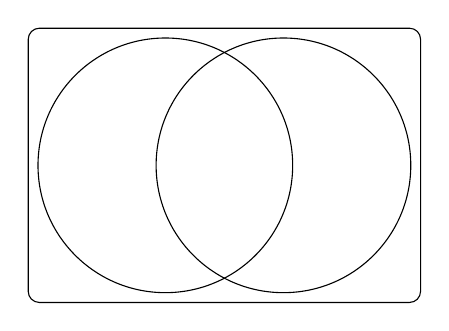
\begin{tikzpicture}
\node (node1) [circle,text width=3cm,draw] at (1,0) {};
\node (node2) [circle,text width=3cm,draw] at (2.5,0) {};
\begin{pgfonlayer}{background}
\node [rounded corners,draw,fit=(node1) (node2)] {};
\end{pgfonlayer}
\end{tikzpicture}
\caption{Venn diagram for two sets (4 regions)}
\label{fig:1}
}
\qquad
\begin{minipage}[t]{0.4\linewidth}
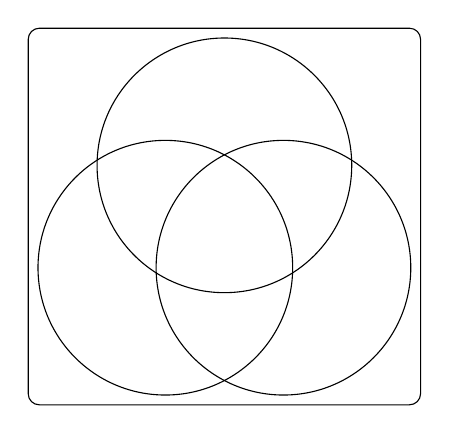
\begin{tikzpicture}
\node (circ1) [circle,text width=3cm,draw] at (0,0) {};
\node (circ2) [circle,text width=3cm,draw] at (1.5,0) {};
\node (circ3) [circle,text width=3cm,draw] at (0.75,1.3) {};
\begin{pgfonlayer}{background}
\node [rounded corners,draw,fit=(circ1) (circ2) (circ3)] {};
\end{pgfonlayer}
\end{tikzpicture}
\caption{Venn diagram for two sets (8 regions)}
\label{fig:2}
\end{minipage}
\end{figure}

Venn diagrams can be used to illustrate set operations by shading the appropriate region in a Venn diagram. For the diagrams in Figure \eqref{fig:20}, set $A$ is represented by the left circle and set $B$ is represented by the right circle.

\begin{figure}[h]
\centering
	\subfigure[][$A\cup B$]{%
		\label{fig:1a}%
		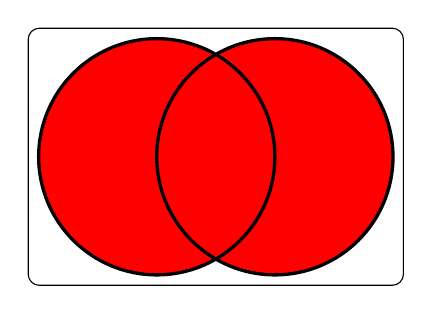
\begin{tikzpicture}[very thick]
		\node (circ1) [circle,text width=3cm,inner sep=0pt,fill=red] at (0,0) {};
		\node (circ2) [circle,text width=3cm,inner sep=0pt,fill=red] at (1.5,0) {};
		\draw (circ2) circle (1.5);
		\draw (circ1) circle (1.5);
		\begin{pgfonlayer}{background}
		\node [rounded corners,draw,fit=(circ1) (circ2)] {};
		\end{pgfonlayer}
		\end{tikzpicture}
		}%
	\qquad
	\subfigure[][$A\cap B$]{%
		\label{fig:2a}%
		\includegraphics[width=4.8cm]{venndiag2}
		}\\
	\subfigure[][$A-B$]{%
		\label{fig:3}%
		\includegraphics[width=4.8cm]{venndiag3}
		}%
	\qquad
	\subfigure[][$A\cap B$]{%
		\label{fig:4}%
		\includegraphics[width=4.8cm]{venndiag4}
		}%
		\caption{Illustrating set operations by shading the appropriate region in a Venn diagram.}
		\label{fig:20}
\end{figure}

\sampleexercise{Examples of set operations illustrated using Venn diagrams:}
\begin{multicols}{2}
\begin{enumerate}
\item $A\cap B\cap C$
\item $(A\cup B)\cap C$
\item $(B-C)-A$
\item $(A-C)\cup B$
\item $(A\cap B)'\cap C'$
\item $C\cap (B-A)'$
\item $[A\cup (B\cap C)]-(B'\cup A)'$
\item $[(B-C)\cup (A-B)]'\cap C$
\end{enumerate}
\end{multicols}

\begin{figure}[h]
\centering
	\subfigure[][$A\cap B\cap C$]{%
		\label{fig:5}%
		\includegraphics[width=3cm]{venndiaga}
		}%
		\hfil
	\subfigure[][$(A\cup B)\cap C$]{%
		\label{fig:6}%
		\includegraphics[width=3cm]{venndiagb}
		}%
		\hfil
	\subfigure[][$(B-C)-A$]{%
		\label{fig:7}%
		\includegraphics[width=3cm]{venndiagc}
		}%
		\hfil
	\subfigure[][$(A-C)\cup B$]{%
		\label{fig:8}%
		\includegraphics[width=3cm]{venndiagd}
		}\\
	\subfigure[][$(A\cap B)'\cap C'$]{%
		\label{fig:9}%
		\includegraphics[width=3cm]{venndiage}
		}%
		\hfil
	\subfigure[][$C\cap (B-A)'$]{%
		\label{fig:10}%
		\includegraphics[width=3cm]{venndiagf}
		}%
		\hfil
	\subfigure[][{$[A\cup (B\cap C)]-(B'\cup A)'$}]{%
		\label{fig:11}%
		\includegraphics[width=3cm]{venndiagg}
		}%
		\hfil
	\subfigure[][{$[(B-C)\cup (A-B)]'\cap C$}]{%
		\label{fig:12}%
		\includegraphics[width=3cm]{venndiagh}
		}%
		\caption{Operations on sets using Venn diagrams.}
		\label{fig:22}
\end{figure}

The results are in in Figures \eqref{fig:5} to \eqref{fig:12}.

It is possible to construct Venn diagrams for more than three sets, but there must be $2^n$ regions on the resulting diagram. See Figure \eqref{fig:21} which shows Venn diagrams for four and five sets.

\begin{figure}[h]
\centering
	\subfigure[][4-set Venn Diagram]{%
		\label{fig:13}%
		\includegraphics[width=3cm]{4setvenn}
		}%
		\hfil
	\subfigure[][4-set Venn Diagram]{%
		\label{fig:14}%
		\includegraphics[width=3cm]{4setvenn2}
		}%
		\hfil
	\subfigure[][5-set Venn Diagram]{%
		\label{fig:15}%
		\includegraphics[width=3cm]{5setvenn}
		}%
		\hfil
	\subfigure[][6-set Venn Diagram]{%
		\label{fig:16}%
		\includegraphics[width=3cm]{5setvenn2}
		}
		\caption{Some Venn diagrams for more than three sets.}
		\label{fig:21}
\end{figure}

\subsection*{Venn Diagram problems}
A common exercise involving Venn diagrams is populating a Venn diagram with values corresponding to the information given in a problem. A sample problem is given below along with step by step instructions on populating the Venn diagram.
It is important to note that the words “or” and “and”, when referring to set operations, denote union and intersection respectively.

\sampleexercise{Example 1}
\begin{quote}
\begin{enumerate}
\item Create a Venn diagram representing the number of students using each online service.

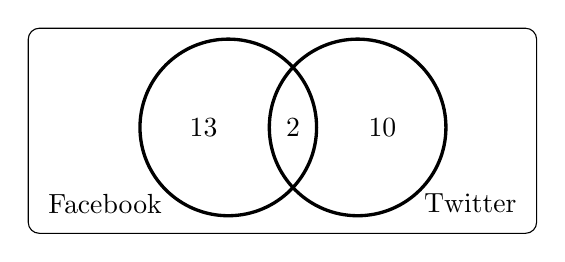
\begin{tikzpicture}[very thick,node distance=1cm]
\node (13) [circle,text width=2cm,draw] {};
\node (10) [circle,text width=2cm,draw] at (13) [right=0.5cm] {};
\node [left] at (13) {13};
\node [right] at (10) {10};
\node at ($(13)!0.5!(10)$) {2};
\node (fb) [below left=1cm] at (13) {Facebook};
\node (tw) [below right=1cm] at (10) {Twitter};
\begin{pgfonlayer}{background}
\node [rounded corners,fit=(fb) (tw) (13) (10),draw] {};
\end{pgfonlayer}
\end{tikzpicture}
\item How many students use both Facebook and Twitter?
\hfill Ans: 2
\end{enumerate}
\end{quote}

\sampleexercise{Example 2}
\begin{quote}
100 people seated at different tables in a party were asked if their group had ordered any of the following items: Pancit, Fried Chicken, or Pork Adobo
\begin{enumerate}
\item 23 people ordered none of these items.
\item 11 people ordered all three of these items.
\item 29 had ordered Fried Chicken or Pork Adobo but did not order Pancit.
\item 41 people ordered Pork Adobo.
\item 46 people ordered at least two of these items.
\item 13 had ordered Pancit and Pork Adobo but not ordered Fried Chicken.
\item 26 people ordered Pancit and Fried Chicken.
\end{enumerate}
Create a Venn diagram representing the number of people who ordered each dish.
\end{quote}
\noindent
\begin{tabularx}{\linewidth}{p{0.6in}@{}@{}p{0.6\linewidth}C}
Step 1 & 
Draw a Venn diagram for the three sets: People who ordered Pancit, Fried Chicken or Pork Adobo.
& \includegraphics[width=\linewidth]{adobo1} \\
Step 2 &
Use the given information to populate regions on your Venn Diagram.
&  \\
 &
“23 people ordered none of these items.”
 & \includegraphics[width=\linewidth]{adobo2} \\
 &
“11 people ordered all three of these items.”

\textit{This statement corresponds to the intersection of all three sets.
}
 & \includegraphics[width=\linewidth]{adobo3} \\
 &
“29 had ordered Fried Chicken or Pork Adobo but did not order Pancit”

\textit{This statement corresponds to the expression $(FC)\cup(Adobo)-(Pancit)$ and the shaded region on the right. We don’t have enough data on the diagram yet to use this piece of information.}
 & \includegraphics[width=\linewidth]{adobo4} \\
	&
“41 people ordered Pork Adobo”

\textit{See the diagram for the region represented by this statement. We don’t have enough data yet to use this information.}
 & \includegraphics[width=\linewidth]{adobo5} \\
 &
“46 people ordered at least two of these items”

\textit{See the diagram for the region represented by this statement. We don’t have enough data yet to use this information.}
 & \includegraphics[width=\linewidth]{adobo6} \\
 &
“13 had ordered Pancit and Pork Adobo but not ordered Fried Chicken”
 & \includegraphics[width=\linewidth]{adobo7} \\
\end{tabularx}

%\noindent
%\begin{tabularx}{\linewidth}{p{0.5in}@{}@{}p{0.6\linewidth}C}
%\end{tabularx}

\begin{tabularx}{\linewidth}{p{0.5in}@{}@{}p{0.6\linewidth}C}
 & 
“26 people ordered Pancit and Fried Chicken”

\textit{Since the statement corresponds to the shaded area on the right, we can conclude that 15 people ordered Pancit and Fried Chicken but NOT Adobo.}
 & \includegraphics[width=\linewidth]{adobo8} \\
 &
We now have enough data to process    Statement 5: “46 people ordered at least two of these items”

\textit{Since the statement corresponds to the shaded area on the right, we can conclude that 7 people ordered both Fried Chicken and Adobo but NOT Pancit.}
 & \includegraphics[width=\linewidth]{adobo9} \\
 &
We can refer again to Statement 4: “41 people ordered Pork Adobo”

\textit{From the data on the diagram, we can conclude that 10 people ordered Pork Adobo only.
}
 & \includegraphics[width=\linewidth]{adobo10} \\
\end{tabularx}

\begin{tabularx}{\linewidth}{p{0.5in}@{}@{}p{0.6\linewidth}C}
 &
Going back to Statement 3: “29 had ordered Fried Chicken or Pork Adobo but did not order Pancit”

\textit{We now have enough data on the diagram to conclude that 12 people ordered Fried Chicken only.}
 & \includegraphics[width=\linewidth]{adobo11} \\
 &
Using the initial information that there are 100 patrons, we can complete the diagram by determining how many customers ordered Pancit only.
 & \includegraphics[width=\linewidth]{adobo12} \\
\end{tabularx}
The completely filled-up Venn Diagram is the final answer.

Here are additional problems on filling up Venn Diagrams:
\begin{enumerate}
\item A study was made of 1000 bodies of water in the country to determine what pollutants were in them.
	\begin{enumerate}
	\item 177 areas were clean
	\item 101 areas were polluted only with crude oil
	\item 439 areas were polluted with phosphates.
	\item 72 areas were polluted with sulfur compound and crude oil, but not with phosphates.
	\item 289 areas were polluted with phosphates, but not with crude oil.
	\item 463 areas were polluted with sulfur compounds.
	\item 137 areas were polluted with only phosphates.
	\end{enumerate}
	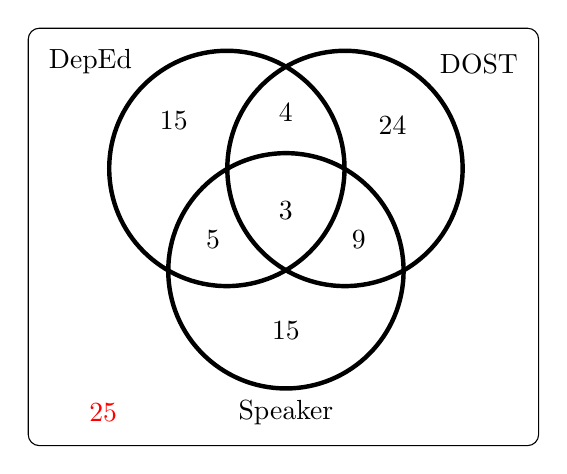
\begin{tikzpicture}[ultra thick]
\node (circ2) [circle,text width=3cm,inner sep=0pt,draw] at (1.5,0) {};
\node (circ3) [circle,text width=3cm,inner sep=0pt,draw] at (0.75,-1.3) {};
\node (circ1) [circle,text width=3cm,inner sep=0pt,draw] at (0,0) {};
\node (A) at ([shift={(135:1.5)}]circ1) [above left] {DepEd};
\node (B) at ([shift={(45:1.5)}]circ2) [above right,align=left] {DOST};
\node (C) at ([shift={(270:1.5)}]circ3) [below] {Speaker};
\node (25) at (C) [left=2cm,red] {25};
\node (3) at (circ3) [above=0.5cm] {3};
\node (9) at ([xshift=5pt]circ2) [below=0.65cm] {9};
\node (5) at ([xshift=-5pt]circ1) [below=0.65cm] {5};
\node (4) at (circ3) [above=1.75cm] {4};
\node (15) at (circ3) [below=0.5cm] {15};
\node (24) at (circ2) [above right=0.4cm] {24};
\node (15) at (circ1) [above left=0.5cm] {15};

\begin{pgfonlayer}{background}
\node [rounded corners,draw,fit=(A) (B) (C)] {};
\end{pgfonlayer}
\end{tikzpicture}
\item 100 students were asked if they knew who any of the following are: The DepEd secretary, The Speaker of the House, and The DOST secretary.
	\begin{enumerate}
	\item 25 people did not know any of these.
	\item 3 people knew all three.
	\item 48 people knew who the Speaker of the House or the DOST secretary were but didn't know who the DepEd secretary was.
	\item 40 people knew who the DOST secretary was.
	\item 21 people knew who at least two of these were.
	\item 7 people knew who the DepEd secretary and the DOST secretary were but didn't know who the Speaker of the House was.
	\item 8 people knew who the DepEd secretary and the Speaker of the House were.
	\end{enumerate}
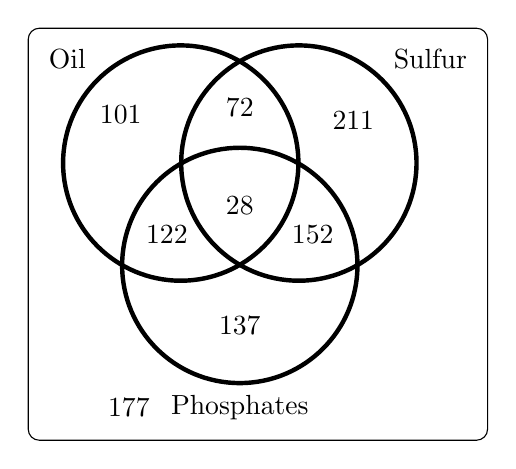
\begin{tikzpicture}[ultra thick]
\node (circ2) [circle,text width=3cm,inner sep=0pt,draw] at (1.5,0) {};
\node (circ3) [circle,text width=3cm,inner sep=0pt,draw] at (0.75,-1.3) {};
\node (circ1) [circle,text width=3cm,inner sep=0pt,draw] at (0,0) {};
\node (A) at ([shift={(135:1.5)}]circ1) [above left] {Oil};
\node (B) at ([shift={(45:1.5)}]circ2) [above right,align=left] {Sulfur};
\node (C) at ([shift={(270:1.5)}]circ3) [below] {Phosphates};
\node (177) at (C) [left=1cm] {177};
\node (28) at (circ3) [above=0.5cm] {28};
\node (152) at ([xshift=5pt]circ2) [below=0.65cm] {152};
\node (122) at ([xshift=-5pt]circ1) [below=0.65cm] {122};
\node (72) at (circ3) [above=1.75cm] {72};
\node (137) at (circ3) [below=0.5cm] {137};
\node (211) at (circ2) [above right=0.4cm] {211};
\node (101) at (circ1) [above left=0.5cm] {101};

\begin{pgfonlayer}{background}
\node [rounded corners,draw,fit=(A) (B) (C)] {};
\end{pgfonlayer}
\end{tikzpicture}
\end{enumerate}

\section*{SUGGESTED ACTIVITIES}
Resource Speakers may choose which class activity will be done by the participants depending on
your level of comfortableness with the activity, available materials, and remaining time.
\subsection*{Activity 1: Constructing a Venn Diagram from a Survey Data}
\subsubsection*{Objectives:}
To construct a Venn Diagram problem based on survey data
\subsubsection*{Preparation:}
Group the participants into 10 groups. Each group is given several minutes to construct a
simple preference survey. (e.g. TV channels they like to watch: kapamilya, kapuso, kapatid;
sports they play: basketball, volleyball, bowling).
\subsubsection*{Activity:}
\begin{enumerate}
\item Each group will survey all the participants based on the survey questions that they constructed. There should be 3 choices and the participants can tick all choices if applicable.
\item After the members of the group surveys ALL the participants, the group tallies the data on a
tally sheet (each group should be provided with a list of all participants).
\item After the tallying all the data, the group constructs the Venn diagram.
\item From the Venn diagram constructed, the group must design a Venn diagram problem.
\item Each group will write down their problem on a sheet of Manila paper and post their
problems on the wall.
\item After the break, groups pair up and solve each others problem.
\item After the alloted time, each group present their solution, and the problems and solutions
are critiqued.
\end{enumerate}
Note: You may use a sample sheet like that found in Figure \eqref{fig:23} For an easier activity instead of 3 choices, 2 choices could be used for the survey.
{\renewcommand{\arraystretch}{1.75}
\begin{figure}
\centering
\begin{tabular}[m]{|l|l|l|l|}
\hline
\multicolumn{4}{|c|}{\LARGE\textbf{SURVEY FORM}}\\
\hline
Name of Participant & Choice 1 & Choice 2 & Choice 3\\ \cline{2-4}
 & & & \\ \hline
1 & & & \\ \hline
2 & & & \\ \hline
3 & & & \\ \hline
4 & & & \\ \hline
5 & & & \\ \hline
6 & & & \\ \hline
7 & & & \\ \hline
8 & & & \\ \hline
9 & & & \\ \hline
10 & & & \\ \hline
\end{tabular}
\caption{Activity 1: Constructing a Venn Diagram from a Survey Data}
\label{fig:23}
\end{figure}
}

\subsection*{Activity 2: Populating a Venn Diagram}
\subsubsection*{Objective:}
 To integrate the Venn Diagram concepts with other subjects taken up by Grade 7 students. For this activity we can integrate some historical facts of SEA nations.

\subsubsection*{Preparation:}
\begin{enumerate}
\item Construct a large Venn Diagram on the classroom floor with tape. Label each circle with a category. For this activity we can use the SEA countries Vietnam, Thailand, and the Philippines.
\item Prepare notecards containing facts about the three countries. Here are some examples, which can be expanded as needed:
\begin{enumerate}
\item Monarchy\hfil	\textit{Thailand only}
\item Colonized by Europeans \hfil		\textit{Vietnam and Philippines}
\item Occupied by Japanese \hfil	\textit{All three countries}
\item Predominantly Christian\hfil \textit{Philippines only}

\end{enumerate}
\item Optional: Pass around a handout containing historical information about these three countries. This can also be coordinated with the History teacher if these topics are already covered.
\end{enumerate}

\subsubsection*{Activity}
\begin{enumerate}
\item Have each student draw from a pile of notecards containing facts about the countries.
\item Randomly select a student to read their fact to the class and then stand in the appropriate area of the Venn Diagram. 
\item Encourage discussion and provide feedback as to the correct placement of the characteristics.
\item Repeat steps 4 and 5 until all students are standing in the correct place in the Venn Diagram (use a model Venn Diagram if necessary).
\item Summarize the results of the activity.
\end{enumerate}
This activity can be revised to integrate Venn diagram concepts with other academic topics like science or literary characters, or things that children enjoy like superhero superpowers.
\subsection*{Activity 3:	Constructing a Venn Diagram Problem}
\subsubsection*{Objectives:}
\begin{enumerate}
\item To construct a Venn Diagram problem based on personal information of the participants/students. 
\item To determine the least amount of information that can be given about a problem that can still be used to populate a Venn Diagram.
\end{enumerate}
\subsubsection*{Preparation:}
Prepare two surveys on personal preferences of students or participants. There should be three possible options for the participants to choose from (actors/actresses, food, subjects, etc.). The participants should be allowed to choose more than one option.
\subsubsection*{Activity:}
\begin{enumerate}
\item Distribute the participants into two groups. Have each group fill up a different survey to generate the data they will need for their Venn Diagram activity.
\item Each group should populate their own Venn Diagrams based on the results of the survey they filled up. A copy of the populated Venn Diagrams are given to the facilitator.
\item On a piece of manila paper, each group should write down phrases that give information about their Venn Diagram. The goal is to give as little information as possible while ensuring that there is enough information to populate a Venn Diagram.
\item The two teams swap information, and they will race to populate the Venn Diagram based on information provided by the other group. The group that completes first is declared the winner.
\item If the losing team can show that it is impossible to populate a Venn Diagram based on the given information, then they are declared the winner instead.
\item The two teams will share their techniques and difficulties encountered in constructing a Venn Diagram problem.
\end{enumerate}


\printbibliography[keyword=Module1,heading=subbibliography,title={REFERENCES}]
\chapter{SET OF REAL NUMBERS}\label{chap:2}
\section*{INTRODUCTION}
This module is designed to describe, represent and compare the different subsets of real
numbers in hierarchical form. Mainly, this module talks about applications of various procedures and
manipulations on the different subsets of the set of real numbers. The topics included in this module
are: definitions of different kinds of numbers; the location of numbers on the number line;
properties of operations (addition and multiplication) that characterizes each set of numbers;
operations involved in each set of numbers (particularly integers and rational numbers); description
and representation of real-life situations involving integers, rational numbers, square roots of
rational numbers and irrational numbers; and solving problems involving real numbers. An
assessment exam and alternative assessment in terms of group activity are also given at the end of
the module.

\section*{OBJECTIVES}
This module is made towards the goal of helping the learners:
\begin{enumerate}
\item Identify the different sets of numbers using properties of operations (addition and
multiplication).
\item Describe and illustrate the absolute value of a number on a number line as the distance of
the number from 0.
\item Perform fundamental operations on integers: addition, subtraction, multiplication, and
division.
\item Define and illustrate rational numbers and arrange them on a number line.
\item Express rational numbers from fraction form to decimal form (both terminating and
repeating) and vice versa.
\item Perform operations on rational numbers and illustrate their properties.
\item Describe principal roots and tell whether they are rational or irrational.
\item Write in scientific notation.
\end{enumerate}

\section*{DISCUSSION}
\subsection*{Numbers and Numerals}
\Bold{Numbers} are ideas that we associate with quantities of things around us. \Bold{Numerals} are the
symbols we use to represent these ideas. Different people use different symbols to represent
numbers. The \Bold{number line} is a line with points and is often used to illustrate order of numbers
because each point which is associated with, or represents a number has a definite location in
relation to other points that also represent other numbers.
\subsection*{The System of Counting Numbers ($\mathbb{N}$)}
\subsubsection*{$\mathbb{N}$ and the Number Line}
Naturally, the first number we use when we count is the number one (1), followed by two (2),
three (3), and so on. We call these numbers \Bold{counting} or \Bold{natural numbers}. The set of counting
numbers is represented by $N = \{1, 2, 3, 4, 5, 6, 7, \ldots\}$. The number line can be used to show the
correct order of these numbers.
\subsubsection*{Subsets of $\mathbb{N}$}
Some of the subsets of the set of natural numbers are the following:
\begin{enumerate}
\item The set of \Bold{prime numbers}. A \Bold{prime number} is a natural number greater than 1 whose only
positive divisors are 1 and itself. Let us represent the set of prime numbers as set $P$.
\[P=\{2,3,5,7,11,13,17,19,\ldots\}\]
\item The set of \Bold{composite numbers}. A \Bold{composite number} is a natural number that has a positive
other than 1 and itself. In other words, a composite number is a natural number greater than 1
that is \textit{not} a prime number. Let us represent the set of composite numbers as set $C$.
\[C = \{4, 6, 8, 9, 10, 12, 14, 15, 16, \ldots\}\]
\item The set of \Bold{odd numbers}. An \Bold{odd number} is a number that is not divisible by 2. Let us represent
the set of odd numbers as set $O$.
\[O = \{1, 3, 5, 7, 9, 11, 13, 15, 17, \ldots\}\]
\item The set of \Bold{even numbers}. An \Bold{even number} is a number that can be divided by 2. Let us represent
the set of even numbers as set $E$.
\[E = \{2, 4, 6, 8, 10, 12, 14, 16, ...\}\]
\end{enumerate}
\subsubsection*{Number Theory}
The basic number theory concepts or terms included in discussing counting numbers are tDivisibility Tests. The method of determining which counting number is divisible by 2, 3, 4, 5, 6,
7, 8, 9, 10, 11, and other numbers.
he
following.
\begin{enumerate}
\item \Bold{Prime Factors}. These are factors that are prime numbers.
\item \Bold{Prime Factorization}. This is the method of expressing a composite number as a product of
primes.
\item \Bold{GCF and LCM}. The methods of finding the \Bold{greatest common factor (GCF)} and \Bold{least common
multiple (LCM)} of certain sets of numbers.
\item \Bold{Divisibility Tests}. The method of determining which counting number is divisible by 2, 3, 4, 5, 6,
7, 8, 9, 10, 11, and other numbers.
\end{enumerate}
\subsubsection*{Properties of Operations ($+$ and $\times$) in $\mathbb{N}$}
The following properties are always true in $\mathbb{N}$.

\begin{tabularx}{\linewidth}{XC}
Property & Examples\\
1. Closure Property for Addition (CLPA) & $1 + 3 = 4, 4 \in N$\\
2. Closure Property for Multiplication (CLPM) & $4 x 5 = 20, 20 \in N$\\
3. Commutative Property for Addition (CPA) & $3+5=5+3$\\
4. Commutative Property for Multiplication (CPM) & $4\times 8=8\times 4$\\
5. Associative Property for Addition (APA) & $(2 + 5) + 3 = 2 + (5 + 3)$\\
6. Associative Property for Multiplication (APM) & $(4 \times 3) \times 2 = 4 \times (3 \times 2)$\\
7. Distributive Property for Multiplication over Addition (DPMA) & $4 \times (5 + 3) = (4 \times 5) + (4 \times 3)$\\
8. Identity Property of Multiplication (IPM) & $8\times1=1\times8=8$\\
\end{tabularx}

\subsection*{The System of Whole Numbers ($\mathbb{W}$)}
\subsubsection*{$\mathbb{W}$ and the Number Line}
Recall from Module \ref{chap:1} when a set has no element, it is called an \Bold{empty set} or a \Bold{null set}. The cardinal number of
the empty set is represented by a number which is called \Bold{zero (0)}. The union of the unit set $\{0\}$ and the set
$\mathbb{N} = \{1, 2, 3, 4, 5, 6, \ldots\}$ is the set of \Bold{whole numbers} represented by $\mathbb{W} = \{0, 1, 2, 3, 4, \ldots\}$. The set $\mathbb N$
is a subset of the set $\mathbb W$, therefore \Ital{all subsets of $\mathbb N$} (i.e., set of prime numbers, set of composite
numbers, set of even numbers, and set of odd numbers) \Ital{are all subsets of $\mathbb W$}.
\subsubsection*{Properties of Operations ($+$ and $\times$) in $\mathbb W$}
\begin{tabularx}{\linewidth}{XC}
Property & Examples\\
1. Closure Property for Addition (CLPA) & $1 + 3 = 4, 4 \in N$\\
2. Closure Property for Multiplication (CLPM) & $4 x 5 = 20, 20 \in N$\\
3. Commutative Property for Addition (CPA) & $3+5=5+3$\\
4. Commutative Property for Multiplication (CPM) & $4\times 8=8\times 4$\\
5. Associative Property for Addition (APA) & $(2 + 5) + 3 = 2 + (5 + 3)$\\
6. Associative Property for Multiplication (APM) & $(4 \times 3) \times 2 = 4 \times (3 \times 2)$\\
7. Distributive Property for Multiplication over Addition (DPMA) & $4 \times (5 + 3) = (4 \times 5) + (4 \times 3)$\\
8. Identity Property of Multiplication (IPM) & $8\times1=1\times8=8$\\
9. Identity Property of Addition (IPA) & $5 + 0 = 0 + 5= 5$\\
\end{tabularx}

\subsection*{The System of Integers ($\mathbb{Z}$)}
\subsubsection*{$\mathbb{Z}$ and the Number Line}
In the sets $\mathbb N$ and $\mathbb W$, subtraction can only be performed by deducting a smaller number from
a larger number. When a larger number is subtracted from a smaller number, the result is a number
that does not belong to these two sets. Another set of numbers called the \Bold{negative numbers}, whose
values are less than zero, is formed. The union of these negative numbers and $\mathbb W$ is called the set of
integers or signed numbers represented by $\mathbb Z = \{\ldots, -4, -3, -2, -1, 0, 1, 2, 3, 4, \ldots\}$. Since $\mathbb W$ is a subset
of $\mathbb Z$, all subsets of W are also subsets of $\mathbb Z$. The number line shows the position of the points that
represent the integers. The order of the numbers depends on their position relative to the point
which represents zero, also called the \Bold{origin}. The \Bold{negative numbers}, also called the \Bold{additive inverses}
of the natural numbers (\Bold{positive numbers}), are located at the left side of zero, while all positive
numbers are located at the right side of zero. Negative numbers are less than zero, while positive
numbers are greater than zero. Zero is neither positive nor negative.
\subsubsection*{Properties of Operations ($+$ and $\times$) in $\mathbb Z$}
The following properties are true in $\mathbb Z$.

\begin{tabularx}{\linewidth}{XC}
Property & Examples\\
1. Closure Property for Addition (CLPA) & $-2+-4=-6,1 + 3 = 4, -6,4 \in \mathbb Z$\\
2. Closure Property for Multiplication (CLPM) & $-3\times 5=-15,4 x 5 = 20, -15,20 \in \mathbb Z$\\
3. Commutative Property for Addition (CPA) & $-3+5=5+-3$\\
4. Commutative Property for Multiplication (CPM) & $4\times -8=-8\times 4$\\
5. Associative Property for Addition (APA) & $(2 + -5) + 3 = 2 + (-5 + 3)$\\
6. Associative Property for Multiplication (APM) & $(-4 \times 3) \times 2 = -4 \times (3 \times 2)$\\
7. Distributive Property for Multiplication over Addition (DPMA) & $-4 \times (5 + 3) = (-4 \times 5) + (-4 \times 3)$, $(5 + 3) \times -4 = (5 \times -4) + (3 \times -4)$\\
8. Identity Property of Multiplication (IPM) & $-8\times1=1\times8=-8$\\
9. Identity Property of Addition (IPA) & $-5 + 0 = 0 + -5 = -5$\\
10. Additive Inverse Property (AIP) & $5 + (-5) = 0$\\
\end{tabularx}
\subsubsection*{Absolute Value of an Integer}
The absolute value of an integer is the distance of the point representing the integer from
the point representing zero. The absolute value of $+5$, represented by $|+5|$, and the absolute value
of $-5$, represented by $|-5|$, are both equal to 5, since the points representing them are both $5$
units away from the point representing 0.
\subsubsection*{Operations on $\mathbb Z$}
\paragraph*{Addition of Integers}
The sum of two integers depends on the signs of both numbers. If the numbers have the
same sign, the sum is preceded by the common sign. If the numbers have different signs, the
difference of the two numbers is taken and the sign of the answer is the sign of the integer with the
greater absolute value.
\begin{example}
\item 
	\begin{inparaenum}
	\item $(+3)+(+4)=(+7)$\hfil \item $(-3) + (-4) = (- 7)$
	\end{inparaenum}
\item 
	\begin{inparaenum}
	\item $(+3) + (-4) = (- 1)$\hfil \item $(-3) + (+4) = (+1)$
	\end{inparaenum}
\end{example}
\paragraph*{Subtraction of Integers}
Subtraction of integers is the addition of the additive inverse of the subtrahend to the
minuend. In symbols, $a - b = a + (-b)$.
\begin{example}
\item $9-3 = 9 + (-3) = 6$
\item $-9 - 3 = -9 + (-3) = -12$
\item $-9 - (-3) = -9 + -(-3) = -9 + 3 = -6$
\item $9 - (-3) = 9 + -(-3) = 9 + 3 = 12$
\end{example}
\paragraph*{Multiplication of Integers}
The product of two integers with the same sign is positive while the product of two integers
with different signs is negative.

\paragraph*{Division of Integers}
The quotient of two integers with the same sign is positive, while the quotient of two
integers with different signs is negative. Zero can never be a divisor.
\subsection*{The System of Rational Numbers $\mathbb Q$}
\subsubsection*{$\mathbb Q$ and the Number Line}
When an integer is divided by another nonzero integer, and the quotient is an integer having no
remainder, the first integer is said to be divisible by the nonzero integer. But what happens when an
integer is divided by a nonzero integer which is not a divisor or a factor of the first integer? The
quotient is definitely not an integer. Another set of numbers is formed which will satisfy the given
condition, and we call this set as the set of \Bold{fractions}. The fractions can either be \Bold{proper} or \Bold{improper}
fractions. The union of the set of integers and the set of fractions is called the set of \Bold{rational
numbers} which is represented by $\mathbb Q = \{\ldots, -4, -7/2, -3, -5/2, -2, -3/2, -1, -1/2, 0, 1/2, 1, 3/2, 2, 5/2, 3,
7/2, 4, \ldots\}$. In other words, a rational number can be expressed as a ratio or quotient of two integers.
All rational numbers can be represented by fractions. Since the set of integers is a subset of the set
of rational numbers, all subsets of the set of integers are also subsets of set $\mathbb Q$. The number line can
be used to show the location of points represented by the rational numbers. %\pdfmarkupcomment[author=Joseph]{Highlight}{Needs some revision.}
\subsubsection*{Properties of Operations ($+$ and $\times$) in $\mathbb Q$}
The following properties are true in $\mathbb Q$.

\begin{tabularx}{\linewidth}{XC}
Property & Examples\\
1. Closure Property for Addition (CLPA) & $-\frac{1}{2}+-\frac{3}{4}=-\frac{5}{4},1+3=4,-\frac{5}{4},4\in \mathbb{Q}$\\
2. Closure Property for Multiplication (CLPM) & $-\frac{3}{4}\times \frac{2}{3}=-\frac{2}{5},4 x 5 = 20, -\frac{2}{5},20 \in \mathbb Q$\\
3. Commutative Property for Addition (CPA) & $-\frac{3}{2}+\frac{5}{4}=\frac{5}{4}+-\frac{3}{2}$\\
4. Commutative Property for Multiplication (CPM) & $\frac{4}{7}\times 8=8\times\frac{4}{7}$\\
5. Associative Property for Addition (APA) & $(\frac{2}{3}+-\frac{5}{2})+3=\frac{2}{3}+(-\frac{5}{2}+3)$\\
6. Associative Property for Multiplication (APM) & $(-\frac{4}{3}\times 3)\times \frac{2}{5}=-\frac{4}{3}\times (3\times \frac{2}{5})$\\
7. Distributive Property for Multiplication over Addition (DPMA) & $-4\times (\frac{5}{2}+\frac{3}{4})=(-4\times\frac{5}{2})+(-4\times\frac{3}{4})$, $(\frac{5}{2}+\frac{3}{4})\times -4=(\frac{5}{2}\times-4)+(\frac{3}{4}\times-4)$\\
8. Identity Property of Multiplication (IPM) & $-\frac{8}{9}\times 1=1\times-\frac{8}{9}=-\frac{8}{9}$\\
9. Identity Property of Addition (IPA) & $-\frac{5}{7}+0=0+-\frac{5}{7}=-\frac{5}{7}$\\
10. Additive Inverse Property (AIP) & $\frac{5}{9}+(-\frac{5}{9}) = 0$\\
11. Multiplicative Inverse Property (MIP) & $2\frac{1}{2}=1$\\
\end{tabularx}

\subsubsection*{Fractions and Decimals}
A subset of $\mathbb Q$ is the set of fractions. A fraction can be defined as the quotient of a whole
number divided by a natural number. A proper fraction has a numerator less than the denominator,
while an improper fraction has a greater numerator than denominator. Any fraction can be
converted to decimal form, either to a terminating or repeating decimal as the case may be.

To convert a fraction to decimal, the numerator is divided by the denominator. A proper
fraction can be converted to either a terminating or repeating decimal. An improper fraction can be
converted to a decimal form with a whole number part, or to a mixed number form. The mixed
number form is a combination of a whole number and a proper fraction.

To convert a terminating decimal to fraction, the decimal is multiplied by a fraction
equivalent to 1 (whose numerator and denominator is a power of 10) and then simplified by dividing
both numerator and denominator by the greatest common factor. For example, 0.45 will be
multiplied by $\frac{100}{100}$, to get $\frac{45}{100}$, which is further simplified to $\frac{9}{20}$.

To convert a repeating decimal to fraction, the following examples can be followed.

\paragraph*{Example 1.} Convert $0.333\ldots$ to fraction.
\paragraph*{Solution.} 
\begin{tabular}{r@{}l}
Let $n\,$ & $=0.333\ldots$\\
$10n\,$ & $=3.333\ldots$\\ \hline
$9n\,$ & $=3$\\
$\therefore n\,$ & $=\frac{1}{3}$\\
\end{tabular}

\paragraph*{Example 2.} Convert $0.4545\ldots$ to a fraction.
\paragraph*{Solution.}
\begin{tabular}{r@{}l}
Let $n\,$ & $= 0.4545\ldots$\\
 $100n\,$ & $= 45. 4545\ldots$\\
  $- n\,$ & $= 0.4545\ldots$\\ \hline
  $99n\,$ & $= 45$\\
  $\therefore n\,$ & $=\frac{5}{11}$\\
\end{tabular}

\paragraph*{Example 3.} Convert $4.3636\ldots$ to a fraction.
\paragraph*{Solution.}
\begin{tabular}{r@{}l}
 Let $n\,$ & $= 4.3636\ldots$\\
  $100n\,$ & $= 436.3636\ldots$\\
   $- n\,$ & $= 4.3636\ldots$\\ \hline
    $99n\,$ & $= 432$\\
   $\therefore n\,$ & $=\frac{48}{11}$\\
\end{tabular}

\subsubsection*{Operations on Natural Numbers}
\paragraph*{Addition and Subtraction}
Rational numbers in fraction form can only be added or subtracted if they have the same
denominators. These fractions are called similar fractions. Always convert dissimilar fractions to
fractions with the same denominators first before adding or subtracting.

\paragraph*{Multiplication}
When multiplying fractions, cancellation can be used to reduce the product to its simplest
form. Cancellation is done by dividing the numerator and denominator by the greatest common
factor.

\paragraph*{Division}
Division of a fraction by another fraction is done by multiplying the dividend by the
reciprocal or multiplicative inverse of the divisor. Then the product is reduced to its simplest
form.

\subsection*{The System of Irrational Numbers $\mathbb{Q'}$}
\subsubsection*{The Set of $\mathbb{Q'}$ and the Number Line}
The numbers that cannot be represented as a ratio of two integers in simplest form are
called irrational numbers. The union of the set of rational numbers and the set of irrational
numbers comprise the set of real numbers which is represented by $\Re$. The set of irrational
numbers is the complement of the set of rational numbers in the universal set of real numbers,
and is represented by
\[\mathbb{Q'}=\{\ldots \sqrt{2},\sqrt{3},\sqrt{5},\sqrt{7},\sqrt{11},\pi,\ldots\}.\]

\subsubsection*{Square Root of a Number as a Rational Number or Irrational Number}
Square roots of numbers sometimes result in rational or irrational numbers.

The square roots of perfect squares, or of fractions having perfect squares in both the
numerator and denominator, are rational numbers.
\begin{example}
\item $\sqrt{49}=\sqrt{7^2}=7$
\item $\sqrt{121}=\sqrt{11^2}=11$
\end{example}
Otherwise, the square roots are irrational numbers.
\subsection*{Scientific Notation}
When writing very large or very small numbers, like the mass of the earth, (6 000
000 000 000 000 000 000 000 kilograms) or the mass of an electron (0.000 000 000 000 000
000 000 000 000 000 911 kilogram), the most convenient form to use is the scientific
notation. In this notation, numbers are represented by the product of a multiplying factor
and a power of ten. A power of ten is the number 10, raised to an integral exponent. The
decimal point is moved until only one nonzero digit is on the left side of it. Then the number
of places the decimal point is moved is used as the exponent of 10. The sign of the exponent
depends on the movement of the decimal point: to the right ($-$) or to the left ($+$).
\begin{example}
\item $6\, 000\, 000\, 000\, 000\, 000\, 000\, 000\, 000\, = 6.0 \times 10^{24}$
\item $0.000\, 000\, 000\, 000\, 000\, 000\, 000\, 000\, 000\, 000\, 911 = 9.11 x 10^{-31}$
\end{example}

\section*{EXERCISES}
\subsection*{Tests for Divisibility.}
Draw {\large\Smiley{}} on the third column if the number in the first column is divisible by the number on the
second column. Otherwise, draw {\large\Frowny{}}.

\noindent
\begin{tabular}{lcl}
1. 67348 & 4 & \hphantom{{\Large\Frowny} answer} \\ \cline{3-3}
2. 73488 & 8 & \\ \cline{3-3}
3. 83671 & 3 & \\ \cline{3-3}
4. 5334 & 6 & \\ \cline{3-3}
5. 5991 & 6 & \\ \cline{3-3}
6. 4425575 & 9 & \\ \cline{3-3}
7. 47830 & 5 & \\ \cline{3-3}
8. 53867 & 11 & \\ \cline{3-3}
9. 1183 & 7 & \\ \cline{3-3}
10. 13855 & 17 & \\ \cline{3-3}
\end{tabular}

\subsection*{Properties of Real Numbers}
\begin{enumerate}
\item How many prime numbers are there from 1 to 50? From 51 to 100? From 101 to 150? From 151
to 200? (Use Sieve of Eratosthenes)
\item How many factors does 72 have? 120? 144? 84? 360?
\item Express each of the following numbers in scientific notation:
	\begin{enumerate}
	\item 45 000 000 000 000 000 000 000 000 000 000
	\item 0.000 000 000 000 000 173
	\item 930 000 000 000 000 000 000
	\item 0.000 000 000 000 000 000 000 000 62
	\item 508 000 000 000 000 000
	\end{enumerate}
\end{enumerate}

\section*{SUGGESTED ACTIVITIES}
\subsection*{Activity 1: Illustrating the Set of Numbers using Venn Diagrams}
\begin{enumerate}
\item Illustrate the relationship of each of the following sets of numbers using the Venn
Diagrams:
	\begin{enumerate}
	\item Prime Numbers and Composite Numbers
	\item Prime Numbers and Even Numbers
	\item Composite Numbers and Odd Numbers
	\item Composite Numbers and Even Numbers
	\item Natural Numbers and Whole Numbers
	\end{enumerate}
\item Show the Hierarchy of the System of Real Numbers using the following:
	\begin{enumerate}
	\item Venn Diagram
	\item Flow Chart
	\item Concept Map
	\end{enumerate}
\end{enumerate}

\subsection*{Activity 2: Categorizing Numbers into the Different Sets}
Check the appropriate boxes that categorize the given numbers.
{\renewcommand{\arraystretch}{1.5}
\begin{center}
\begin{tabular}{|l|c|c|c|c|c|c|}
\hline 
Number & $\mathbb N$ & $\mathbb W$ & $\mathbb Z$ & $\mathbb Q$ & $\mathbb{Q’}$ & $\Re$ \\ \hline \hline
$45.9$ & \hphantom{check} & \hphantom{check} & \hphantom{check} & \hphantom{check} & \hphantom{check} & \hphantom{check} \\ \hline
$-1\,444$  & & & & & & \\ \hline
$3\sqrt{6}$  & & & & & & \\ \hline
$\frac{5}{9}$  & & & & & & \\ \hline
$125\%$  & & & & & & \\ \hline
$27.5$  & & & & & & \\ \hline
$3\, 678\, 125$  & & & & & & \\ \hline
$5\sqrt{2693}$  & & & & & & \\ \hline
$8.246$  & & & & & & \\ \hline
$7\sqrt{9}$  & & & & & & \\ \hline
\end{tabular}
\end{center}
}

\subsection*{Activity 3: The Boat is Sinking (Divisibility Version)}
\subsubsection*{Objective:}
To practice divisibility rules in a fun way.
\subsubsection*{Preparation:}
Each participant is given a sheet of paper (can be a scratch paper) and they should write
their favourite one digit on the sheet of paper (it should be large enough to occupy the
whole sheet).
\subsubsection*{Activity:}
\begin{enumerate}
\item The resource person calls on the participants (just like in the party game, “The Boat is
Sinking”) to group themselves (using their own one-digit numbers as digit) to form numbers
like:
	\begin{enumerate}
	\item two-digit numbers divisible by 2
	\item three-digit numbers divisible by 3
	\item four-digit numbers divisible by 4
	\item five-digit numbers divisible by 5
	\end{enumerate}
\item Participants that cannot form groups will be disqualified from the activity. After some time,
remaining participants are declared winners.
\end{enumerate}
\subsection*{Activity 4: Words of Wisdom}
\subsubsection*{Objectives:}
To be able to conduct a drill on arithmetic (operations on integers).
\subsubsection*{Preparation:}
Each participant is given a copy of the worksheet.
\subsubsection*{Activity:}
\begin{enumerate}
\item After each participant has a copy of the worksheet, the resource person announces the
operation for each column: Col A ($\times$), Col B ($-$), Col C ($+$) and Col D ($\div$).
\item The worksheet is quite self-explanatory. If they have found “the phrase” and they are
satisfied, they may ask the resource person if they are correct.
\item After the allotted time, the worksheet’s answers are revealed.
\end{enumerate}
%\newpage
\vfill 
\def\Cline{\cline{1-1} \cline{3-6} \cline{8-11} \cline{13-16} \cline{18-21}}
\begin{center}
{\LARGE\bfseries WORDS OF WISDOM (\textit{an arithmetic drill})}\\[24pt]
{\Large\bfseries PART 1: BASIC ARITHMETIC}\\[5pt]
Using the indicated operation, compute as fast as you can but do not be careless.\\
\begin{tabular}{|c|@{}c@{}|c|c|c|c|@{}c@{}|c|c|c|c|@{}c@{}|c|c|c|c|@{}c@{}|c|c|c|c|}
\Cline
Row & \hphantom{=} & \multicolumn{2}{c|}{} &  & Col A & \hphantom{=} & \multicolumn{2}{c|}{} & & Col B & \hphantom{=} & \multicolumn{2}{c|}{} &  & Col C & \hphantom{=} & \multicolumn{2}{c|}{} & & Col D\\ \Cline
1 & & 1 & 6 & = & & & 2 & 1 & = & & & 3 & 6 & = & & & 21 & 7 & = & \\ \Cline
2 & & 2 & 7 & = & & & 3 & 6 & = & & & 2 & 1 & = & & & 36 & 6 & = & \\ \Cline
3 & & 3 & 8 & = & & & 2 & 7 & = & & & 4 & 6 & = & & & 27 & 3 & = & \\ \Cline
4 & & 2 & 2 & = & & & 4 & 8 & = & & & 7 & 7 & = & & & 48 & 8 & = & \\ \Cline
5 & & 4 & 4 & = & & & 7 & 2 & = & & & 8 & 8 & = & & & 72 & 9 & = & \\ \Cline
6 & & 7 & 3 & = & & & 8 & 4 & = & & & 6 & 2 & = & & & 84 & 4 & = & \\ \Cline
7 & & 8 & 5 & = & & & 6 & 3 & = & & & 5 & 4 & = & & & 63 & 7 & = & \\ \Cline
8 & & 6 & 9 & = & & & 5 & 5 & = & & & 3 & 3 & = & & & 55 & 5 & = & \\ \Cline
9 & & 4 & 6 & = & & & 3 & 9 & = & & & 1 & 5 & = & & & 39 & 3 & = & \\ \Cline
10 & & 3 & 1 & = & & & 1 & 6 & = & & & 2 & 9 & = & & & 16 & 2 & = & \\ \Cline
\end{tabular}

\vspace{12pt}
{\Large\bfseries PART 2: FROM NUMBERS TO LETTERS TO\\[5pt] WORDS}\\[5pt]
From Part 1, compute from the corresponding column and row.\\
Convert the value to the corresponding letter in the standard English alphabet. (e.g. 1 $\rightarrow$ A, 2 $\rightarrow$ B)
Then, rearrange the letters to form a word.\\[24pt]

\def\CLine{\cline{1-4} \cline{6-9} \cline{11-14} \cline{16-19}}
\begin{tabular}{|c|@{}c@{}|c|c|@{}c@{}|c|@{}c@{}|c|c|@{}c@{}|c|@{}c@{}|c|c|@{}c@{}|c|@{}c@{}|c|c|}
\CLine
\multicolumn{4}{|c|}{WORD 1} & \hphantom{=} & \multicolumn{4}{c|}{WORD 2} & \hphantom{=} & \multicolumn{4}{c|}{WORD 4} & \hphantom{=} & \multicolumn{4}{c|}{WORD 6}\\ \CLine
A4+D6 & = & \hphantom{NO} & \hphantom{NO} & & C7/C1 & = & \hphantom{NO} & \hphantom{NO} & & A1$\star$D1 & = & \hphantom{NO} & \hphantom{NO} & & D7+D8 & = & \hphantom{NO} & \hphantom{NO}\\ \CLine
A2+C8 & = & \hphantom{NO} & \hphantom{NO} & & D6/C2 & = & \hphantom{NO} & \hphantom{NO} & & C3-B3 & = & \hphantom{NO} & \hphantom{NO} & & B7/C2 & = & \hphantom{NO} & \hphantom{NO}\\ \CLine
B1$\star$C1 & = & \hphantom{NO} & \hphantom{NO} & & B2$\star$B9 & = & \hphantom{NO} & \hphantom{NO} & & A9-C6 & = & \hphantom{NO} & \hphantom{NO} & & A10-B4 & = & \hphantom{NO} & \hphantom{NO}\\ \CLine
A1+D4 & = & \hphantom{NO} & \hphantom{NO} & & A6-A5 & = & \hphantom{NO} & \hphantom{NO} & & A7$\star$D5 & = & \hphantom{NO} & \hphantom{NO} & & C10-C8 & = & \hphantom{NO} & \hphantom{NO}\\ \CLine
B4+D9 & = & \hphantom{NO} & \hphantom{NO} & & B6/C5 & = & \hphantom{NO} & \hphantom{NO} & & C4+D3 & = & \hphantom{NO} & \hphantom{NO} & & A10$\star$C9 & = & \hphantom{NO} & \hphantom{NO}\\ \CLine
D5/B6 & = & \hphantom{NO} & \hphantom{NO} & & WORD & \multicolumn{3}{c|}{} & & WORD & \multicolumn{3}{c|}{} & & WORD & \multicolumn{3}{c|}{}\\ \CLine
B7/D4 & = & \hphantom{NO} & \hphantom{NO} & \multicolumn{15}{c}{}\\ \cline{1-4} \cline{6-9} \cline{11-14}
A9+B10 & = & & & & \multicolumn{4}{c|}{WORD 3} & & \multicolumn{4}{c|}{WORD 5} & \multicolumn{5}{c}{}\\ \cline{1-4} \cline{6-9} \cline{11-14}
D7-B3 & = & & & & D10-B8 &=& & & & C6+C10 &=& & & \multicolumn{5}{c}{}\\ \cline{1-4} \cline{6-9} \cline{11-14}
B5$\star$C2 & = & & & & A8/C9 &=& & & & A3-D8 &=& & & \multicolumn{5}{c}{}\\ \cline{1-4} \cline{6-9} \cline{11-14}
C3+D2 & = & & & & A4$\star$B5 &=& & & & A6-D2 &=& & & \multicolumn{5}{c}{}\\ \cline{1-4} \cline{6-9} \cline{11-14}
A3+B10 & = & & & & A2+C7 &=& & & & B1$\star$D1 &=& & & \multicolumn{5}{c}{}\\ \cline{1-4} \cline{6-9} \cline{11-14}
C4-D3 & = & & & & WORD & \multicolumn{3}{c|}{} & & C6+C10 &=& & & \multicolumn{5}{c}{}\\ \cline{1-4} \cline{6-9} \cline{11-14}
C2$\star$C9 & = & & & \multicolumn{5}{c}{} & & WORD & \multicolumn{3}{c|}{} & \multicolumn{5}{c}{}\\ \cline{1-9} \cline{11-14}
WORD & \multicolumn{8}{c|}{} & \multicolumn{10}{c}{}\\ \cline{1-9}
\end{tabular}

\vspace{12pt}
{\Large\bfseries PART 3: FROM WORDS TO A PHRASE}\\[5pt]

Rearrange the words in part 2 to form a phrase.\\[12pt]

\hrulefill
\end{center}

\printbibliography[keyword=Module2,heading=subbibliography,title={REFERENCES}]
\chapter{MEASUREMENT}\label{chap:3}

\section*{INTRODUCTION}
This module presents a discussion on measurement that includes key concepts like definition
of measurement, development of measurement from primitive to present times, uses and
importance of measurement, systems of measurement, types of measurements such as linear
measures, liquid measures (capacity/volume), and mass or weight. Conversion factors from one unit
to another either within a system or from one system to another are also discussed. Measurement
of time, temperature, and utilities usage (meter reading) are also included. Solving problems using
the formulas on measurement of geometric figures such as perimeter, area, and volume are also
explored.
\section*{OBJECTIVES}
After completing this module, the learner should be able to extend concepts of measurements
to include different types of measures and all the subsets of the set of real numbers to solve
measurement problem. In particular, the learner should be able to:
\begin{enumerate}
\item describe what it means to measure;
\item describe the development of measurement from the primitive to the present international
system of units;
\item convert measurements from one unit to another for each type of measurement including
the English system;
\item estimate or approximate the measures of quantities particularly length, weight/mass,
volume/capacity, time, angle and temperature (use of instruments);
\item use appropriate instruments to measure quantities such as length, weight/mass, volume,
time, angle, and temperature; and
\item solve problems involving formulas in finding perimeter, area, and volume.
\end{enumerate}
\section*{DISCUSSION}
\subsection*{Motivation}
Answer the following questions.
\begin{enumerate}
\item Which of the following line segments is the longest? Which is the shortest?

\begin{tikzpicture}
\draw (0,0) -- (2,0);
\node [below] at (0,0) {A};
\node [below] at (2,0) {B};
\begin{scope}[xshift=3cm]
\draw (0,0) -- (3,0);
\node [below] at (0,0) {C};
\node [below] at (3,0) {D};
  \begin{scope}[xshift=4cm]
	\draw (0,0) -- (1.5,0);
	\node [below] at (0,0) {E};
	\node [below] at (1.5,0) {F};
	\end{scope}
\end{scope}
\end{tikzpicture}
\item Which of the given figures occupy more space than the others?

\begin{tikzpicture}
\draw (0,0) rectangle (3,2);
\begin{scope}[xshift=4cm]
\draw (0,0) -- (1.5,1) -- (3,0) -- cycle;
	\begin{scope}[xshift=4cm,yshift=-1cm]
	\draw (0,0) rectangle (3,3);
	\end{scope}
\end{scope}
\end{tikzpicture}
\item Which of the given containers have more liquid than the others?

\begin{tikzpicture}
\draw (0,0) ellipse (2 and 0.5);
\draw (-2,0) -- (-2,-2);
\draw (-2,-2) arc (180:360:2 and 0.5);
\draw (2,-2) -- (2,0);
	\begin{scope}[xshift=4cm]
	\draw (0,0) ellipse (1.5 and 0.5);
	\draw (-1.5,0) -- (-1.5,-3);
	\draw (-1.5,-3) arc (180:360:1.5 and 0.5);
	\draw (1.5,-3) -- (1.5,0);	
		\begin{scope}[xshift=3.5cm]
		\draw (0,0) ellipse (1.25 and 0.5);
		\draw (-1.25,0) -- (-1.25,-3.5);
		\draw (-1.25,-3.5) arc (180:360:1.25 and 0.5);
		\draw (1.25,-3.5) -- (1.25,0);	
		\end{scope}
	\end{scope}
\end{tikzpicture}
\end{enumerate}
How do you answer these questions? To be able to answer these questions you need to
compare one figure with the other figures. Then you compare also the quantities or the
properties of these figures. The process of comparing one quantity with another quantity is
known as \Bold{measurement}.

\begin{definition}[Measurement]
\Bold{Measurement} is a quantitative description of a fundamental property or physical
phenomenon. When measuring, comparison of an unknown quantity with a certain
standard called \Bold{unit of measurement} is being done.

The science of measurement is called \Bold{metrology}. The English word \Ital{measurement}
originates from the Latin \Ital{m\-ens\-ura} and the verb \Ital{metiri} through the Middle French \Ital{mesure}.
\end{definition}

\subsection*{Historical Background}
Standard units of measurement were already used in ancient times. It evolved over
the course of human history to help prevent problems on fraud in commerce. Laws
regulating measurement were developed so that communities would have certain common
benchmarks. Generally, units of measurement are essentially arbitrary; groups of people
make them up as the need arises, and then agree on certain standards when they use them.

Ancient people used human body parts (arms, hands, feet) to measure length. The
width of a finger was called a \Bold{finger} or \Bold{digit}. Another unit of measure used was the \Bold{palm}
which was the width of a person’s four fingers excluding the thumb. A \Bold{span} was the width of
three palms. The \Bold{cubit} was described as the distance from a man’s elbow to the tip of his
middle finger. Genesis 6: 15 of the Bible stated that Noah’s ark was 300 cubits long, 50
cubits wide and 30 cubits high. One cubit was equivalent to seven palms. The width of a
person’s thumb was called \Bold{uncia}. One foot was equivalent to twelve uncias. The \Bold{yard}, based
on the distance from the tip of a person’s nose to the tip of his middle finger, was
equivalent to three feet. Ancient people also used the \Bold{king’s foot} as the standard unit of
measure for buying, selling, and trading as long as the king ruled. A \Bold{fathom} was the distance
from one outstretched hand to the other, and was equivalent to four cubits.

Eventually, size variations of the different body parts created measurement
problems. Different measurements would be given for the same length using the same unit.
To eliminate such confusion, international conventions were conducted to set standard
units of measure.

\subsection*{International Treaties (Optional)}
Units of measurement are generally defined on a scientific basis as overseen by
governmental or supra-governmental agencies, and established in international treaties.
\Bold{The General Conference on Weights and Measures (CGPM)} which was established in 1875
by the Treaty of the meter oversees the \Bold{International System of Units (SI)} and has custody
of the \Bold{International Prototype Kilogram}. The \Bold{meter} was redefined in 1983 by the CGPM as
the \Ital{distance traveled by light in free space in 1/299,792,458 of a second} while in 1960 the
\Bold{international yard} was defined by the governments of the United States, United Kingdom,
Australia and South Africa as being \Ital{exactly} 0.9144 meters.

In the United States, the \Bold{National Institute of Standards and Technology (NIST)}, a
division of the United States Department of Commerce, regulates commercial
measurements. In the United Kingdom, the one doing this job is the National Physical
Laboratory (NPL). In Australia it is done by the Commonwealth Scientific and Industrial
Research Organization. In South Africa the one doing this is the Council for Scientific and
Industrial Research, while in India the National Physical Laboratory of India does this job.

\subsection*{Units and Systems of Measurement}
\begin{figure}[h]
\centering
\includegraphics[width=2in]{milkbottle}
\caption{A baby bottle that measures in all three measurement systems, Imperial (U.K.), U.S. customary, and
metric.}
\label{fig3:1}
\end{figure}

\begin{figure}[h]
\centering
\includegraphics[width=2in]{measuringdev}
\caption{Four measuring devices having metric calibrations}
\label{fig3:2}
\end{figure}

\subsection*{Linear Measures}
To measure lengths or distances, linear measures are used. An inch is the smallest
and commonly used linear unit in the English system. In this system, other units such as foot,
yard, and mile are used for longer distances. In the metric system the basic unit of length is
the meter. The meter is the basis of other units of measurements such as the decimeter,
centimeter and millimeter. To measure longer distances, the decameter, hectometer and
kilometer are used.

\subsection*{Liquid Measures}
To measure volume (the space occupied by a liquid substance), liquid measures are
used. The basic liquid measures in the English system are the fluid ounce and the gallon. In
the metric system, liter is the basic unit.

\subsection*{The Dry Measure}
The dry measure is used for measuring grains, fruits, vegetables, and the like. The
English system uses pints and quarts as the units for dry measures and for liquid measures.
The metric system also uses the same unit for measuring both liquid and dry substances.

\subsection*{Mass and Weight}
Mass was used by Newton to mean the quantity of matter, and it mass manifests
itself gravitationally and inertially. The earth’s gravitational pull on an object depends on the
object’s mass. The greater the mass of the object, the stronger the earth’s gravitational pull
on it. Mass depends only on the number and kinds of atoms that compose an object. It
does not depend on location. The amount of material in an object remains the same
whether it is located on Earth, on the moon or in outer space. Mass is also a measure of the
inertia of an object. The greater the mass of an object, the greater is its inertia and the more
force is needed to change its state of motion. Mass is measured in ounces (oz), pounds (lb)
and tons in the English system, while it is measured in grams (g) and kilograma (kg) in the
metric system.

Weight is described as a force. Weight is the earth’s gravitational force acting on an
object. It is measured in Newtons (N) like any other force. It depends on the object’s
location and how strongly the object is attracted by the earth’s gravity. The weight of an
object in a place without gravity would be zero.

Mass and weight are different from each other. Mass is the amount of matter in an
object while weight is how that matter is strongly attracted by the force of gravity.
Moreover, mass does not change and does not depend on the location, while weight varies
with location. However, they are proportional to each other in a certain place. Greater
masses have greater weights while smaller masses have smaller weights. This is the reason
why in some cases, mass and weight are used interchangeably. In free fall, (no net
gravitational forces) objects lack weight but retain their mass.

One device for measuring weight or mass is called a weighing \Ital{scale} or, often, simply
a scale. A spring scale measures force but not mass, and a balance compares weight. Both
require a gravitational field to operate. Some of the most accurate instruments for
measuring weight or mass are based on load cells with a digital read-out, but require a
gravitational field to function and would not work in free fall.

\section*{English Customary Weights and Measures}
\subsection*{Linear Measure or Distance}
Short distance units in all traditional measuring systems are based on the dimensions
of the human body. The inch represents the width of a thumb; in many languages, the word
for "inch" is also the word for "thumb." The foot (12 inches) was originally the length of a
human foot, but has evolved to be longer than most people's feet. The yard (3 feet) was
used in England as the name of a 3-foot measuring stick, but it is also understood to be the
distance from the tip of the nose to the end of the middle finger of the outstretched hand. If
you stretch your arms out to the sides as far as possible, your total "arm span," from one
fingertip to the other, is a fathom (6 feet).

Based on history, many other "natural units" of the same kind were used such as the
following: the digit (the width of a finger, 0.75 inch), the nail (length of the last two joints of
the middle finger, 3 digits or 2.25 inches), the palm (width of the palm, 3 inches), the hand
(4 inches), the shaftment (width of the hand and outstretched thumb, 2 palms or 6 inches),
the span (width of the outstretched hand, from the tip of the thumb to the tip of the little
finger, 3 palms or 9 inches), and the cubit (length of the forearm, 18 inches).

\subsection*{Mass/Weight}
The basic traditional unit of weight, the pound, originated as a Roman unit and was
used throughout the Roman Empire. The Roman pound was divided into 12 ounces, but
many European merchants preferred to use a larger pound of 16 ounces, perhaps because a
16-ounce pound is conveniently divided into halves, quarters, or eighths. During the Middle
Ages there were many different pound standards in use, some of 12 ounces and some of 16.
The use of these weight units naturally followed trade routes, since merchants trading along
a certain route had to be familiar with the units used at both ends of the trip.

The oldest English weight system has been used since the time of the Saxon kings. It
is based on the 12-ounce troy pound, which provided the basis on which coins were minted
and gold and silver were weighed. Since Roman coins were still in circulation in Saxon times,
the troy system was designed to model the Roman system directly. The troy pound weighs
5760 grains, and the ounces weigh 480 grains. Twenty pennies weighed an ounce, and
therefore a pennyweight is $480/20 = 24$ grains. The troy system continued to be used by
jewelers and also by druggists until the nineteenth century. Even today gold and silver prices
are quoted by the troy ounce in financial markets everywhere.

Since the troy pound was smaller than the commercial pound units used in most of
Europe, medieval English merchants often used a larger pound called the "mercantile"
pound (\LATIN{libra mercatoria}). This unit contained 15 troy ounces, so it weighed 7200 grains. This
unit seemed about the right size to merchants, but its division into 15 parts, rather than 12
or 16, was very inconvenient. Around 1300 the mercantile pound was replaced in English
commerce by the 16-ounce avoirdupois pound. This is the pound unit still in common use in
the U.S. and Britain. Modeled on a common Italian pound unit of the late thirteenth century,
the avoirdupois pound weighs exactly 7000 grains. The avoirdupois ounce, 1/16 pound, is
divided further into 16 drams.

Unfortunately, the two English ounce units don't agree: the avoirdupois ounce is
$7000/16 = 437.5$ grains while the troy ounce is $5760/12 = 480$ grains. Conversion between
troy and avoirdupois units is so awkward, no one wanted to do it. The troy system quickly
became highly specialized, used only for precious metals and for pharmaceuticals, while the
avoirdupois pound was used for everything else.

\subsection*{Liquid Measure or Capacity or Volume}
The names of the traditional volume units are the names of standard containers.
Until the eighteenth century, it was very difficult to measure the capacity of a container
accurately in cubic units, so the standard containers were defined by specifying the weight
of a particular substance, such as wheat or beer, that they could carry. Thus the gallon, the
basic English unit of volume, was originally the volume of eight pounds of wheat. This
custom led to a multiplicity of units, as different commodities were carried in containers of
slightly different sizes.

Gallons are always divided into 4 quarts, which are further divided into 2 pints each.
For larger volumes of dry commodities, there are 2 gallons in a peck and 4 pecks in a bushel.
Larger volumes of liquids were carried in barrels, hogsheads, or other containers whose size
in gallons tended to vary with the commodity, with wine units being different from beer and
ale units or units for other liquids.

For liquids Americans preferred to use the traditional British wine gallon, which
Parliament defined to equal exactly 231 cubic inches in 1707. As a result, the U.S. volume
system includes both "dry" and "liquid" units, with the dry units being about 1/6 larger than
the corresponding liquid units.

On both sides of the Atlantic, smaller volumes of liquid are traditionally measured in
fluid ounces, which are at least roughly equal to the volume of one ounce of water. To
accomplish this in the different systems, the smaller U.S. pint is divided into 16 fluid ounces,
and the larger British pint is divided into 20 fluid ounces.

On both sides of the Atlantic, smaller volumes of liquid are traditionally measured in
fluid ounces, which are at least roughly equal to the volume of one ounce of water. To
accomplish this in the different systems, the smaller U.S. pint is divided into 16 fluid ounces,
and the larger British pint is divided into 20 fluid ounces.

Because of their many eccentricities, English customary units clearly are more
cumbersome to use than metric units in trade and in science. As metrication proceeds, they
are less and less in use. On the other hand, these traditional units are rich in cultural
significance. We can trace their long histories in their names and relationships.

The units of measure of length, volume and mass /weight in English system are given
in the Table \eqref{chap3tab:1} below. These units are used as conversion factors from one unit of measure to
another.

\begin{table}
\centering
\caption{English System of Measurement}
\begin{tabular}{ll}
\hline
\hline
Linear Measures & Equivalent Unit Measure\\
\hline \hline
12 inches (in) & 1 foot (ft)\\
3 feet & 1 yard (yd)\\
$5\frac{1}{2}$ yards & 1 rod\\
40 rods & 1 furlong\\
8 furlongs & 1 statute mile\\
3 miles & 1 league\\
3 inches & 1 palm\\
4 inches & 1 hand\\
6 inches & 1 span\\
18 inches & 1 cubit\\
21.8 inches & 1 Bible cubit\\
$2\frac{1}{2}$ feet &1 military pace\\
5, 280 feet or 1,760 yards & 1 mile\\
\hline
\hline
Liquid Measures & Equivalent Unit Measures\\
\hline \hline
2 cups (c) & 1 pint\\
2 pints (pt) & 1 quart\\
4 quarts (qt) & 1 gallon (gal)\\
3 teaspoons (tsp) & 1 tablespoon (tbs)\\
8 fluid ounces (fl. oz) & 1 cup\\
16 fluid ounces & 1 pint\\
\hline
\hline
Dry Measures & Equivalent Unit Measures\\
\hline \hline
\multicolumn{2}{c}{(Used for measuring grains, fruits, vegetables, etc.)}\\
2 pints & 1 quart\\
8 quarts & 1 peck(pk)\\
4 pecks & 1 bushel (bu)\\
4 quarts & 1 gallon\\
\hline
\hline
Measures of Mass /Weight & Equivalent Unit Measures\\
\hline \hline
Avoirdupois Weight & \\
27 11/32 grams & 1 dram\\
16 drams &1 ounce (oz)\\
28.3495 grams &1 ounce\\
16 ounces &1 pound (lb)\\
454 grams &1 pound\\
28 pounds &1 quarter (qtr)\\
4 quarters &1 cwt\\
2,000 pounds &1 short ton\\
2,240 pounds &1 long ton\\
\hline
\hline
Troy Weight & Equivalent Unit Measure\\
\hline \hline
24 grains & 1 pennyweight (pwt)\\
20 pennyweight & 1 ounce\\
12 ounces & 1 pound\\
\multicolumn{2}{c}{(Used for weighing gold, silver and jewels)}\\
\hline
\end{tabular}
\label{chap3tab:1}
\end{table}

\subsection*{The Metric System}
The metric system is a decimal system of measurement based on its units for length,
the meter and for mass, the kilogram. It exists in several variations, with different choices of
base units. Since the 1960s, the International System of Units (SI) is the internationally
recognized metric system. Metric units of mass, length, and electricity are widely used
around the world for both everyday and scientific purposes.

The metric system features a single base unit for many physical quantities. Other
quantities are derived from the standard SI units. Multiples and fractions of the units are
expressed as powers of 10 of each unit. Unit conversions are always simple because they
are in the ratio of ten, one hundred, one thousand, etc, so that convenient magnitudes for
measurements are achieved by simply moving the decimal place: 1.234 meters is 1234
millimeters or 0.001234 kilometers. The use of fractions, such as 2/5 of a meter, is not
prohibited, but uncommon. All lengths and distances, for example, are measured in meters,
or thousandths of a meter (millimeters), or thousands of meters (kilometers). There is no
profusion of different units with different conversion factors as in the Imperial system which
uses, for example, inches, feet, yards, fathoms, rods.

The metric system replaces all the traditional units, except the units of time and of
angle measure, with units satisfying three conditions:

\begin{enumerate}
\item One fundamental unit is defined for each quantity. These units are now defined precisely
in the International System of Units.
\item Multiples and fractions of these fundamental units are created by adding prefixes to the
names of the defined units. These prefixes denote powers of ten, so that metric units are
always divided into tens, hundreds, thousands, etc. The original prefixes included milli- for
1/1,000, centi- for 1/100, deci- for 1/10, deka- for 10, hecto- for 100, and kilo- for 1,000.
\item The fundamental units are defined rationally and are related to each other in a rational
fashion.
\end{enumerate}

The metric units were defined in a different way from any traditional units of
measure. The Earth was selected as the “measuring stick”. The meter was defined to be one
ten-millionth of the distance from the Equator to the North Pole. The liter was to be the
volume of one cubic decimeter, and the kilogram was to be the weight of a liter of pure
water.

The metric system was first proposed in 1791. It was adopted by the French
revolutionary assembly in 1795, and the first metric standards (a standard meter bar and
kilogram bar) were adopted in 1799. There was considerable resistance to the system at
first, and its use was not made compulsory in France until 1837. The first countries to
actually require use of the metric system were Belgium, the Netherlands, and Luxembourg,
in 1820.

The units of measure of length, volume and mass/weight in metric system are given in
the Table \eqref{chap3tab:2} below. These units are used as conversion factors from one unit of measure to
another. Dekameter decameter

\begin{table}
\centering
\caption{Metric System}
\begin{tabular}{ll}
\hline \hline
Linear Measures & Equivalent Unit Measure\\
\hline
10 millimeters (mm) & 1 centimeter (cm)\\
10 centimeters & 1 decimeter (dm)\\
10 decimeters & 1 meter (m)\\
100 centimeters & 1 meter\\
1,000 millimeters & 1 meter\\
10 meters &1 decameter (dkm)\\
10 decameters &1 hectometer (hm)\\
100 meters &1 hectometer\\
10 hectometers &1 kilometer (km)\\
1,000 meters &1 kilometer\\
\hline
 & \\
\hline
\hline
Liquid Measures &Equivalent Unit Measures\\
\hline
10 milliliters (ml) &1 centiliter (cl)\\
10 centiliters &1 deciliter (dl)\\
10 deciliters &1 liter (l)\\
100 centiliters &1 liter\\
1,000 milliliters &1 liter\\
10 liters &1 decaliter (dkl)\\
10 decaliters &1 hectoliter (hl)\\
10 hectoliters &1 kiloliter (kl)\\
1 cubic centimeter (cc) &1 milliliter (ml)\\
1,000 cubic centimeters &1,000 milliliters\\
1,000 milliliters &1 liter\\
1,000 liters &1 cubic meter (m$^3$)\\
\hline
& \\
\hline
\hline
Measures of Mass /Weight &Equivalent Unit Measures\\
\hline
10 milligrams &1 centigram (cg)\\
10 centigrams &1 decigram (dg)\\
10 decigrams &1 gram (g)\\
100 centigrams &1 gram\\
1,000 milligrams &1 gram\\
10 grams &1 decagram (dkg)\\
10 decagrams &1 hectogram (hg)\\
100 grams &1 hectogram\\
10 hectograms &1 kilogram (kg)\\
100 kilograms &1 quintal (ql)\\
10 quintals &1 ton (t)\\
\hline
\end{tabular}
\label{chap3tab:2}
\end{table}

\subsection*{International System of Units}
The International System of Units (abbreviated as SI from the French language name
\Ital{Système International d'Unités}) is the modern revision of the metric system. It is the world's
most widely used system of units, both in everyday commerce and in science. The SI was
developed in 1960 from the meter-kilogram-second (MKS) system, rather than the
centimeter-gram-second (CGS) system, which, in turn, had many variants. During its
development, the SI also introduced several newly named units that were previously not a
part of the metric system. The original SI units for the six basic physical quantities were:
\begin{center}
\begin{tabular}{ll}
meter (m) &SI unit of length\\
second (s) &SI unit of time\\
kilogram (kg) &SI unit of mass\\
ampere (A) &SI unit of electric current\\
degree Kelvin (K) &SI unit of thermodynamic temperature\\
candela (cd) & SI unit of luminous intensity\\
\end{tabular}
\end{center}
The mole was subsequently added to this list and the degree Kelvin renamed the kelvin.

There are two types of SI units, base units and derived units. Base units are the
simple measurements for time, length, mass, temperature, amount of substance, electric
current and light intensity. Derived units are constructed from the base units, for example,
the watt, i.e. the unit for power, is defined from the base units as m$^2\cdot$kg$\cdot$s$^{-3}$. Other physical
properties may be measured in compound units, such as material density, measured in
kg/m$^3$.

\subsubsection*{Converting Prefixes}
The SI allows easy multiplication when switching among units having the same base
but different prefixes. To convert from meters to centimeters it is only necessary to multiply
the number of meters by 100, since there are 100 centimeters in a meter. Inversely, to
switch from centimeters to meters one multiplies the number of centimeters by 0.01 or
divide centimeters by 100.

\subsubsection*{Length}
\begin{figure}[!h]
\centering
\includegraphics[width=2in]{ruler}
\caption{A 2-metre carpenter's ruler}
\label{chap3fig:1}
\end{figure}

A ruler or rule is a tool used in, for example, geometry, technical drawing,
engineering, and carpentry, to measure lengths or distances or to draw straight lines.
Strictly speaking, the \Ital{ruler} is the instrument used to \Bold{rule} straight lines and the calibrated
instrument used for determining length is called a \Ital{measure}, however common usage calls
both instruments \Ital{rulers} and the special name \Ital{straightedge} is used for an unmarked rule.
The use of the word \Ital{measure}, in the sense of a measuring instrument, only survives in the
phrase \Ital{tape measure}, an instrument that can be used to measure but cannot be used to
draw straight lines. As can be seen in the photographs on this page, a two-meter carpenter's
rule can be folded down to a length of only 20 centimeters, to easily fit in a pocket, and a
five-meter-long tape measure easily retracts to fit within a small housing.

\subsubsection*{Some Special Names}
We also use some special names for some multiples of some units as in Table \eqref{chap3tab:3}
\begin{table}[!h]
\centering
\caption{SI Special Names}
\begin{tabular}{ll}
\hline \hline
100 kilograms & 1 quintal\\
1000 kilogram & 1 metric tonne\\
10 years & 1 decade\\
100 years & 1 century\\
1000 years & 1 millennium\\
\hline
\end{tabular}
\label{chap3tab:3}
\end{table}

\subsubsection*{Difficulties}
Since accurate measurement is essential in many fields, and since all measurements are
necessarily approximations, a great deal of effort must be taken to make measurements as
accurate as possible. For example, consider the problem of measuring the time it takes an
object to fall a distance of one meter (about 39 in). Using physics, it can be shown that, in
the gravitational field of the Earth, it should take any object about 0.45 second to fall one
meter. However, the following are just some of the sources of error that arise:
\begin{enumerate}
\item This computation used for the acceleration of gravity 9.8 meters per second squared
(32 ft/s$^2$). But this measurement is not exact, but only precise to two significant
digits.
\item The Earth's gravitational field varies slightly depending on height above sea level and
other factors.
\item The computation of 0.45 second involved extracting a square root, a mathematical
operation that required rounding off to some number of significant digits, in this
case two significant digits.
\end{enumerate}
So far, we have only considered scientific sources of error. In actual practice, dropping
an object from a height of a meter stick and using a stopwatch to time its fall, we have other
sources of error:
\begin{enumerate}
\item Most common, is simple carelessness.
\item Determining the exact time at which the object is released and the exact time it hits
the ground. There is also the problem that the measurement of the height and the
measurement of the time both involve some error.
\item Air resistance
\end{enumerate}
Scientific experiments must be carried out with great care to eliminate as much error as
possible, and to keep error estimates realistic.

\subsection*{Metric-English Relationship}
Table \eqref{chap3tab:4} shows the comparison between the Metric and English Systems of
Measurements.
\begin{table}[!h]
\centering
\caption{Metric-English Conversions}
\begin{tabular}{ll}
\hline \hline
Linear Measures &Equivalent Measure\\
\hline
Metric & English\\
1 millimeter & 0.04 inches\\
1 centimeter & 0.39 inches\\
1 decimeter & 3.94 inches\\
1 meter & 39.37 inches\\
1 meter & 3.28 feet\\
1 meter & 1.09 yards\\
1 decameter & 32.81 feet\\
1 hectometer & 328.08 feet\\
1 kilometer & 3,280.80 feet\\
1 kilometer & 0.62 mile\\
25.40 millimeter & 1 inch\\
2.54 centimeters & 1 inch\\
0.03 meter & 1 inch\\
0.30 meter & 1 foot\\
0.91 meter & 1 yard\\
1.61 kilometers & 1 mile\\
\hline
 & \\
\hline \hline
Liquid Measures & Equivalent Measures\\
\hline
Metric &English\\
1 milliliter & 0.03 fluid ounce\\
1 centiliter &0.34 fluid ounce\\
1 deciliter &3.38 fluid ounce\\
1 liter &1.06 liquid quarts\\
1 liter &0.91 dry quart\\
1 decaliter &2.64 gallons\\
1 hectoliter &26.42 gallons\\
1 kiloliter &264.18 gallons\\
0.95 liter &1 liquid quart\\
1.10 liters &1 dry quart\\
3.80 liter &1 gallon\\
\hline
 & \\
\hline \hline
Measures of Mass &Equivalent Measures\\
\hline
Metric &English\\
1 milligram &0.02 grain\\
1 centigram &0.15 grain\\
1 decigram &1.54 grains\\
1 gram &0.04 ounce\\
1 decagram &0.35 ounce\\
1 hectogram &3.53 ounces\\
1 kilogram &2.20 pounds\\
1 metric ton &2,204.62 pounds\\
1 metric ton &1.10 tons\\
28.35 grams &1 ounce\\
0.45 kilogram &1 pound\\
0.91 metric ton &1 ton\\
\hline
\end{tabular}
\label{chap3tab:4}
\end{table}

\subsubsection*{Conversion from One Unit to Another}
The following illustrative examples show how to convert one measure from one unit to
another.
\subsubsubsection{English Units of Measure}
\begin{example}
\item Convert 7 yards to feet. Conversion factor: 1 yd $= 3$ ft

Solution: $7\yd\cdot \dfrac{3\ft}{1\yd}=\boxed{21\ft}$

\item Convert 72 inches to feet. Conversion factor: 1 ft $= 12$ in

Solution: $72\mathrm{in}\cdot\dfrac{1\mathrm{ft}}{12\IN}=\boxed{6\ft}$

\item Convert 14.25 gallons to quarts. Conversion factor: 1 gal $= 4$ qt

Solution: $14.2\gal\cdot\dfrac{4\qt}{1\gal}=\boxed{57\qt}$
\end{example}
\subsubsubsection{Metric Units of Measure}
\begin{example}
\item Convert 8 meters to centimeters. Conversion factor: 1 m $= 100$ cm

Solution: $8\m\cdot \dfrac{100\cm}{1\m}=\boxed{800\cm}$

\item Convert 3 liters to millimeters. Conversion factor: $1 \Li = 1000 \mL$

Solution: $3\Li\cdot\dfrac{1000\mL}{1\Li}=\boxed{3,000\mL}$

\item Convert 250 millimeters to decimeters. Conversion factors: $1 \cm = 10 \mm$, $1\dm = 10
\cm$, hence, $1 \dm = 100 \m$

Solution: $250\mm\cdot\dfrac{1\cm}{10\mm}\cdot\dfrac{1\dm}{10\cm}=\boxed{2.5\dm}$

\item Convert 4,625 centimeters to meters. Conversion factor: $1 \m = 100 \cm$

Solution: $4,625\cm\cdot\dfrac{1\m}{100\cm}=\boxed{46.25\m}$
\end{example}

\subsubsubsection{Metric to English and Vice Versa}
\begin{example}
\item Convert 12 meters to yards. Conversion factor: $1 \m = 1.09 \yd$

Solution: $12\m\cdot\dfrac{1.09\yd}{1\m}=\boxed{13.08\yd}$

\item Convert 10 miles to meters. Conversion factor: $1 \mi = 1.61 \km$, $1 \km = 1000 \m$

Solution: $10\mi\cdot\dfrac{1.61\km}{1\mi}\cdot\dfrac{1000\m}{1\km}=\boxed{16,100\m}$

\item Convert $400 \oz$ to grams. Conversion factor: $1 \oz = 28.35 \g$

Solution: $400\oz\cdot\dfrac{28.35\g}{10\oz}=\boxed{11,340\g}$
\end{example}

\subsection*{Exercises}
\begin{enumerate}[A.]
\item Write the abbreviations of the following units of measure.
	\begin{multicols}{3}
	\begin{enumerate}[1.]
	\item foot
	\item meter
	\item inch
	\item hectometer
	\item millimeter
	\item kilometer
	\item yard
	\item mile
	\item gallon
	\item pint
	\item liter
	\item pound
	\item ounces
	\item grain
	\item millimeter
	\end{enumerate}
	\end{multicols}
\item Write either weight, linear, time, or capacity in each blank to denote the type of measure.
	\begin{multicols}{2}
	\begin{enumerate}[1.]
	\item \answerline{foot}
	\item \answerline{gallon}
	\item \answerline{pint}
	\item \answerline{yard}
	\item \answerline{gram}
	\item \answerline{cup}
	\item \answerline{liter}
	\item \answerline{peck}
	\item \answerline{day}
	\item \answerline{century}
	\end{enumerate}
	\end{multicols}
\item Fill in the blank with the correct number.
	\begin{enumerate}[1.]
	\item \Line $\ft=1\yd$
	\item \Line $\T = 1\yd$
	\item \Line $\dm = 1\m$
	\item \Line $\IN = 1 \yd$
	\item \Line $\ft = 1 \mi$
	\item \Line $\m = 1 \dkm$
	\item \Line $\cm = 1 \dm$
	\item \Line $\dm = 1 \km$
	\end{enumerate}
\item Convert. Use mixed numbers or decimals if necessary.
	\begin{multicols}{2}
	\begin{enumerate}[1.]
	\item $24 \yd = \Line \ft$
	\item $6 \mi = \Line \yd$
	\item 72 in =  ft
	\item 17 ft = \Line in
	\item 7 mi = \Line ft
	\item 1/4 mi = \Line yd
	\item 90 in = \Line yd
	\item 7 ft = \Line yd
	\item 6 mi = \Line in
	\item 14 m = \Line dm
	\item 85 km = \Line dkm
	\item 12 mm = \Line m
	\item 8 m = \Line cm
	\item 1hm = \Line m
	\item 45 m = \Line hm
	\item 83.5 km = \Line hm
	\item 47 dm = \Line m
	\item 145 km = \Line m
	\item 15 ft = \Line  in
	\item 3/4 ft = \Line in
	\item 1.3 mi = \Line ft
	\item 380,160 = \Line mi
	\end{enumerate}
	\end{multicols}
\end{enumerate}

\subsubsection*{Perimeter}
Perimeter is the measure of the total distance around a plane figure. To find the
perimeter of any polygon, the lengths of the sides are added. There are formulas that are
used to make the computation easier and faster.

Table \eqref{chap3tab:5} shows most common shapes and the formula to find the
perimeter of each figure.

\begin{table}[!h]
\centering
\begin{tabularx}{\linewidth}{XXX}
\hline
\hline
Figure & Formula & Description\\
\hline
1. Triangle & $P=a+b+c$ & $a$, $b$, and $c$ are the lengths of
the sides\\
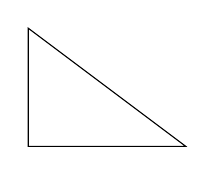
\begin{tikzpicture}
\draw (0,0) -- (2,0) -- (0,1.5) -- cycle;
\end{tikzpicture}
&  & \\
2. Trapezoid & & \\
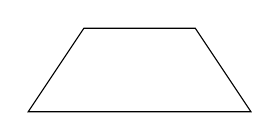
\begin{tikzpicture}[xscale=2]
\draw (0,0) +(135:0.5cm) -- +(45:0.5cm) -- +(-45:1cm) -- +(-135:1cm) -- cycle;
\end{tikzpicture}
 & $P = b_1 + b_2 + s_1 + s_2$ & $b_1$ and $b_2$ are the bases or
parallel sides while $s_1$ and $s_2$
are the nonparallel sides\\
3. Parallelogram & & \\
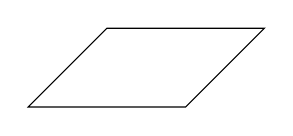
\begin{tikzpicture}
\draw (0,0) -- (2,0) -- (1,-1) -- (-1,-1) -- cycle;
\end{tikzpicture}
 & $P = 2l + 2w$ & $l$ is the length and $w$ is the
width of the parallelogram\\
3. Rectangle & & \\
\tikz \draw (0,0) rectangle (2.5,1.5); & $P = 2L + 2W$ & $L$ is the length and $W$ is the width of the rectangle\\
4. Square & & \\
\tikz \draw (0,0) rectangle (2,2); & $P = 4s$ & $s$ is the length of side of the
square \\
5. Circle & & \\
\tikz \draw (0,0) circle (1cm); & $C=2\pi r=\pi d$ & $r$ is the radius of the circle and $d$ is the diameter; $\pi \approx 3.14$\\
\hline
\end{tabularx}
\caption{Note: A circle is a plane figure whose perimeter is known as the circumference of the circle.}
\label{chap3tab:5}
\end{table}
%\newpage
\subsection*{Exercises}
Find the perimeter of the following.
\begin{multicols}{2}
\begin{enumerate}
\item Square

\begin{tikzpicture}
\draw (0,0) rectangle (2.25,2.25);
\path (0,0) -- (0,2.25) node [midway, left]  {6 cm};
\end{tikzpicture}

\item Rectangle 

\begin{tikzpicture}[scale=1.25]
\draw (0,0) rectangle (2.5,1.25);
\path (0,0) -- (0,1.25) node [midway,left] {3 m};
\path (0,1.25) -- (2.5,1.25) node [midway, above] {6 m};
\end{tikzpicture}

\item Triangle 

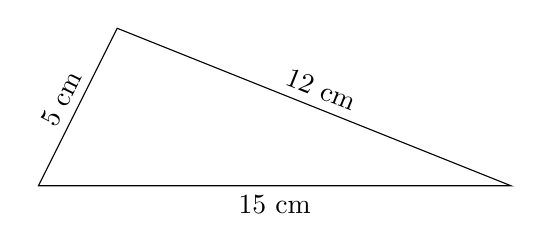
\begin{tikzpicture}[scale=2]
\draw (0,0) -- (3,0) -- (0.5,1) -- cycle;
\path (0,0) -- (0.5,1) node [midway,above,sloped] {5 cm};
\path (0,0) -- (3,0) node [midway, below] {15 cm};
\path (0.5,1) -- (3,0) node [midway, above, sloped] {12 cm};
\end{tikzpicture}

\item Isosceles Trapezoid

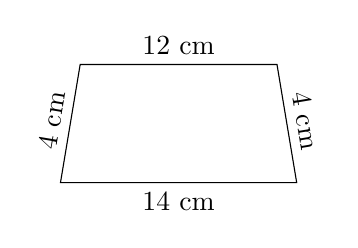
\begin{tikzpicture}
\draw (0,0) -- (3,0) -- (2.75,1.5) -- (0.25,1.5) -- cycle;
\path (0,0) -- (3,0) node [midway,below] {14 cm};
\path (3,0) -- (2.75,1.5) node [midway, above,sloped] {4 cm};
\path (0.25,1.5) -- (2.75,1.5) node [midway,above] {12 cm};
\path (0,0) -- (0.25,1.5) node [midway, above, sloped] {4 cm};
\end{tikzpicture}
\end{enumerate}
\end{multicols}

\subsubsubsection{Area}
The area of a plane figure is the total number of unit regions occupied or contained
in the given plane figure. The unit region is expressed in square units.

\begin{example}
\item The rectangle below has width = 3 units, length = 5 units. There are 15 square
units in the figure. Therefore, the area of the rectangle is 15 square units.

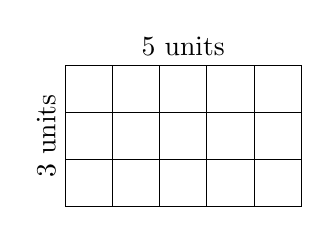
\begin{tikzpicture}[scale=0.6]
\draw (0,0) grid (5,3);
\path (0,3) -- (5,3) node [above, midway] {5 units};
\path (0,0) -- (0,3) node [midway, above, sloped] {3 units};
\end{tikzpicture}
\end{example}

Table \eqref{chap3tab:6} shows most common shapes and the formula to find the area of
each figure.

{\renewcommand{\arraystretch}{1.5}
\begin{table}[!h]
\centering
\caption{Formulas for Areas of Some Common Shapes}
\begin{tabularx}{\linewidth}{XXX}
\hline
\hline
1. Triangle & $A=\dfrac{bh}{2}$ & $A$ is the area, $b$ is the base
and $h$ is the height or
altitude\\
2. Square & $A=s^2$ & $s$ is the length of the side\\
3. Rectangle & $A=lw$ & $l$ is the length and $w$ is the
width\\
4. Parallelogram & $A=bh$ & $b$ is the base and $h$ is the
height or altitude\\
5. Trapezoid & $A=\dfrac{h(b_1+b+2)}{2}$ & $h$ is the altitude and $b_1$ and $b_2$ are the bases\\
6. Circle & $A=\pi r^2$ & $r$ is the radius of the circle; $\pi \approx 3.14$\\
\hline
\end{tabularx}
\label{chap3tab:6}
\end{table}}

\subsection*{Exercises}
Find the area of the following figures:
\begin{enumerate}
\item A square whose side is 9 cm.
\item A rectangle whose width is 2 m and whose length is 5 m.
\item A triangle whose height is 2 cm and whose base is 8 cm.
\item A circle whose diameter is 20 ft.
\item A trapezoid with a height of 8 cm and bases 6 cm and 9 cm.
\end{enumerate}

\subsubsubsection{Volume}
If we want to find how much a box or any container will hold, we need a
measurement of a space. Space involves three dimensions: length, width and height. Any
figure that represents a space is three-dimensional and the measurement of this space is
called volume. The volume is measured in cubic units.

The standard English cubic measures are the cubic inch, cubic foot and the cubic yard.

\begin{center}
1 cubic foot (cu. ft) = 1,728 cubic inches (cu. in)\\
1 cubic yard (cu. yd) = 27 cubic feet (cu. ft)
\end{center}

The standard metric cubic measures are the cubic centimeters and the cubic meters.

Table \eqref{chap3tab:7} shows the formula that are used to solve for the volume of some regular solids.

\begin{table}[!h]
\centering
\caption{Formulas for Volumes of Regular Solids}
\begin{tabularx}{\linewidth}{XXX}
\hline \hline
Figure & Formula & Meaning of Symbols\\
\hline
1. Cube & & \\
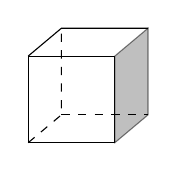
\begin{tikzpicture}[scale=1.1]
\draw (0,0) rectangle (1,1);
\draw [fill=gray,opacity=0.5] (1,0) -- ++(40:0.5cm) -- ++(0,1) -- ++(220:0.5cm) -- cycle;
\draw [dashed] (0,0) -- ++(40:0.5cm) -- ++(0,1);
\draw (0,1) -- ++(40:0.5cm) -- ++(1,0);
\draw [shift=(40:0.5cm),dashed] (0,0) -- (1,0);
\end{tikzpicture}
 & $V=s^3$ & $V=$ volume; $s=$ length of edge\\
2. Rectangular solid & & \\
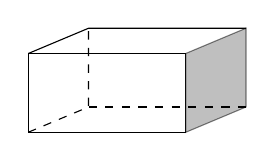
\begin{tikzpicture}[scale=1,xscale=2]
\draw (0,0) rectangle (1,1);
\draw [fill=gray,opacity=0.5] (1,0) -- ++(40:0.5cm) -- ++(0,1) -- ++(220:0.5cm) -- cycle;
\draw [dashed] (0,0) -- ++(40:0.5cm) -- ++(0,1);
\draw (0,1) -- ++(40:0.5cm) -- ++(1,0);
\draw [shift=(40:0.5cm),dashed] (0,0) -- (1,0);
\end{tikzpicture}
 & $V=lwh$ & $V=$ volume; $l=$ length; $w=$ width; $h=$ height\\
3. Square Pyramid & & \\
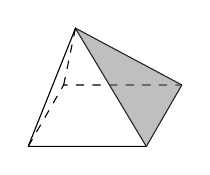
\begin{tikzpicture}[scale=0.6]
\draw (0,0) -- (2.5,0) -- ++(60:1.5cm);
\draw [dashed] (0,0) -- ++(60:1.5cm) -- ++(2.5,0);
\draw (0,0) -- (1,2.5) -- (2.5,0)
							 (1,2.5) -- ($(2.5,0)+(60:1.5cm)$);
\fill [fill=gray,opacity=0.5] (2.5,0) -- ($(2.5,0)+(60:1.5cm)$) -- (1,2.5) -- cycle;
\draw [dashed] (1,2.5) -- ($(0,0)+(60:1.5cm)$);
\end{tikzpicture}
 & $V=\frac{1}{3}lwh$ & $V=$ volume; $l=$ length; $w=$ width; $h=$ height\\
4. Circular Cylinder & & \\
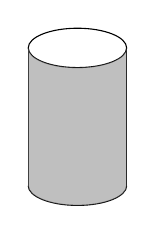
\begin{tikzpicture}[scale=0.5]
		\draw (0,0) ellipse (1.25 and 0.5);
		\draw (-1.25,0) -- (-1.25,-3.5);
		\draw (-1.25,-3.5) arc (180:360:1.25 and 0.5);
		\draw (1.25,-3.5) -- (1.25,0);	
		\fill [gray,opacity=0.5] (-1.25,0) -- (-1.25,-3.5) arc (180:360:1.25 and 0.5) -- (1.25,0) arc (0:180:1.25 and -0.5);
\end{tikzpicture}
 & $V=\pi r^2 h$ & $V=$ volume; $r=$ radius; $h=$ height \\
5. Cone & & \\
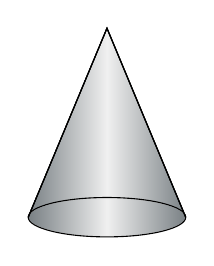
\begin{tikzpicture}[scale=1]
\draw [draw=white,left color=insideo,right color=insideo,middle color=insidei] (0,0) ellipse (1 and 0.25);
\shade [left color=insideo,right color=insideo,middle color=insidei] (-1,0) arc (180:360:1 and -0.25) -- (0,2.4) -- cycle;
\draw (-1,0) -- (0,2.4) -- (1,0);
\draw (-1,0) arc (180:360:1 and 0.25) -- (0,2.4) -- cycle;
\draw (-1,0) arc (180:360:1 and -0.25) -- (0,2.4) -- cycle;
\end{tikzpicture}
 & $V=\frac{1}{3}\pi r^2h$ & $V=$ volume; $r=$ radius; $h=$ height \\
6. Sphere & & \\
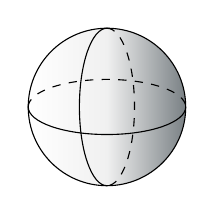
\begin{tikzpicture}
\draw [left color=white,right color=insideo,middle color=insidei] (0,0) circle (1cm);
\draw (-1,0) arc (180:360:1cm and 0.35cm);
\draw [dashed] (-1,0) arc (180:360:1cm and -0.35cm);
	\begin{scope}[rotate=-90]
	\draw (-1,0) arc (180:360:1cm and 0.35cm);
	\draw [dashed] (-1,0) arc (180:360:1cm and -0.35cm);
	\end{scope}
\end{tikzpicture}
 & $V=\frac{4}{3}\pi r^3$ & $V=$ volume; $r=$ radius; $\pi\approx 3.14$ \\
\hline
\end{tabularx}
\label{chap3tab:7}
\end{table}

\subsubsubsection{Time Measure}
Table \eqref{chap3tab:8} shows the units used to measure time.

\begin{table}[!h]
\centering
\caption{Units of Time}
\begin{tabular}{ll}
\hline \hline
Time Measures & Equivalent Unit Measure\\
\hline
60 seconds & 1 minute\\
60 minutes & 1 hour\\
24 hours & 1 day\\
7 days & 1 week\\
28,29,30 or 31 days & 1 calendar month\\
30 days & 1 month (computing interest)\\
365 days & 1 year\\
366 days & 1 leap year\\
\hline
\end{tabular}
\label{chap3tab:8}
\end{table}

Time reading is done through a clock with 12 numbers on it. The two hands are
called the minute hand and the hour hand. The hour hand indicates the hour reading and
the minute hand represents the minute reading. Some clock has a second hand that reads
the second.

\subsubsubsection{Temperature}
There are two thermometer scales that are commonly used to measure temperature.
These are the Fahrenheit (F) and the Centigrade or Celsius (C). The two scales give
temperature readings in degrees ($^{\circ}$).

\begin{example}
\item $45^{\circ}$ F is read as “forty-five degrees Fahrenheit”
\item $20^{\circ}$ C is read as “twenty degrees Centigrade”
\end{example}

The freezing point of water on the Fahrenheit scale is $32^{\circ}$ F while the boiling point of
water is $212^{\circ}$ F. On the Centigrade scale, the freezing point of water is $0^{\circ}$ C while the boiling
point is $100^{\circ}$. The thermometer is the instrument used to measure temperature.

To change one unit of measure to another unit, we use formulas. The formula used
to change Fahrenheit to Centigrade or Celsius is
\begin{equation}
\mathrm{C}=\frac{5}{9}(\mathrm{F}-32)
\end{equation}
\begin{example}
\item Change $59\degree\F$ to $\degree\C$.

Solution:
\begin{align*}
\C&=\frac{5}{9}(\F-32)\\
&=\frac{5}{9}(27)\\
&=\boxed{15}
\end{align*}
Therefore, $59\degree\F=15\degree\C$.
\end{example}
To change Centigrade to Fahrenheit, we use the formula
\begin{equation}
\F=\frac{9}{5}\C+32
\end{equation}
\begin{example}
\item Change $20\degree\C$ to $\degree\F$

Solution: 
\begin{align*}
\F&=\frac{9}{5}\C+32\\
&=\frac{9}{5}(20)+32\\
&=36+32\\
&=\boxed{68}
\end{align*}
Therefore, $20\degree\C=68\degree\F$.
\end{example}
\subsection*{Exercises}
\begin{enumerate}[A.]
\item Change each of the following to $\degree\C$.
\begin{multicols}{2}
\begin{enumerate}[1.]
\item 72\degree\F.
\item 120\degree\F.
\item 160\degree\F.
\item 84\degree\F.
\item 98\degree\F.
\item 130\degree\F.
\end{enumerate}
\end{multicols}
\item Change each of the following to \degree\F.
\begin{multicols}{2}
\begin{enumerate}[1.]
\item 12\degree\C.
\item 30\degree\C.
\item 35\degree\C.
\item 94\degree\C.
\item 98\degree\C.
\item 75\degree\C.
\end{enumerate}
\end{multicols}
\end{enumerate}

\section*{WORKSHOP ACTIVITIES}
\subsection*{Activity 1: Exercises on Problem Solving Involving Measurements}
\begin{enumerate}
\item If one side of a regular pentagon is 7 cm long, what is its perimeter? (Hint: A regular pentagon has 5 equal sides.)
\item The diameter of a bicycle tire is 50 cm. What is the circumference of the tire?
\item The perimeter of a square is 48 cm. How long is each side?
\item A large pizza has a circumference of 215.2 cm. What is its diameter?
\item The diameter of a wheel is 72 cm. Find its circumference.

Find the area of each of the following by subdividing it into common shapes.
\begin{multicols}{3}
\item 
\begin{tikzpicture}
\draw (0,0) -- (1,0) -- (1,1.5) -- (-0.5,1.5) -- (-0.5,1) -- (0,1) -- cycle;
\path (0,0) -- (1,0) node [below,midway] {2};
\path (0,0) -- (0,1) node [left,midway] {2};
\path (-0.5,1) -- (-0.5,1.5) node [left,midway] {1};
\end{tikzpicture}
\item 
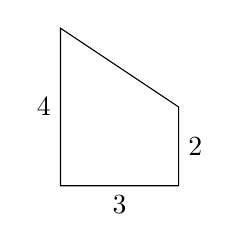
\begin{tikzpicture}[scale=0.5]
\draw (0,0) -- (3,0) -- (3,2) -- (0,4) -- cycle;
\path (0,0) -- (0,4) node [left,midway] {4};
\path (0,0) -- (3,0) node [below,midway] {3};
\path (3,0) -- (3,2) node [right,midway] {2};
\end{tikzpicture}
\item 
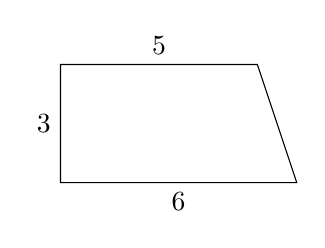
\begin{tikzpicture}[scale=0.5]
\draw (0,0) -- (0,3) -- (5,3) -- (6,0) -- cycle;
\path (0,0) -- (0,3) node [left, midway] {3};
\path (0,3) -- (5,3) node [above, midway] {5};
\path (0,0) -- (6,0) node [below, midway] {6};
\end{tikzpicture}
\end{multicols}
\item Which is warmer, 48\degree\C or 112\degree\F?
\item Which is colder, 18\degree\C or 53 \degree\F?
\item What is the melting point of gold in \degree\F if its melting point is 1,115 \degree\C?
\item What is the melting point of silver in \degree\C if its melting point is 1,814 \degree\F?
\end{enumerate}

\subsection*{Activity 2: Math Trail}
\subsection*{Objective:}
To apply measurement skills, conversion, and problem solving in real-life situations.
\subsection*{Preparation:}
Group the participants into groups. Each group is oriented on the rules of the “Math Trail”/Amazing Race”.
\subsection*{Instructions:}
Using the same materials (e.g. ruler, meterstick, protractor, calculator), each group will race
in a specified area (an auditorium or field) to do tasks (e.g. measure, compute) in a given
time limit.
\subsection*{Sample Task 1:}
Assume that the figures drawn are a square and a circle.
Find the area of the shaded region rounded to the nearest $\mm^2$.
\begin{figure}[!h]
\centering
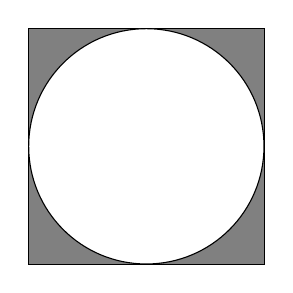
\begin{tikzpicture}[scale=1.5]
\draw [fill=gray] (-1,-1) -- (1,-1) -- (1,1) -- (-1,1) -- cycle;
\node (a) [circle, text width=3cm, inner sep=0pt,draw,fill=white] {};
\end{tikzpicture}
\end{figure}

\subsection*{Sample Task 2:}

Assume that the figures drawn are a triangle and a circle.

Find the volume of the cylinder whose base radius is the same as
the circumference of the circle and whose height is the same as the
perimeter of the triangle (rounded to the nearest $\mL$).\\

\begin{figure}[!h]
\centering
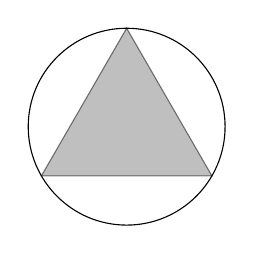
\begin{tikzpicture}[scale=2.5]
\coordinate (a) at ($(0,0)+(90:0.5cm)$);
\coordinate (b) at ($(0,0)+(-30:0.5cm)$);
\coordinate (c) at ($(0,0)+(-150:0.5cm)$);
\draw [fill=gray,opacity=0.5] (a) -- (b) -- (c) -- cycle;
\draw (0,0) circle (0.5cm);
\end{tikzpicture}
\end{figure}

\printbibliography[keyword=Module3,heading=subbibliography,title={REFERENCES}]
\chapter{ALGEBRAIC MANIPULATIONS AND COMMON MISCONCEPTIONS}
\section*{INTRODUCTION}
This module presents common misconceptions of students in using GEMDAS in their algebra
classes, and some mental math and shortcuts in addition, subtraction, multiplication and division.
Also, we review the properties of real numbers as a field, rules on exponents, and hierarchy of
operations. Examples, exercises, and oral assessment are also given at the end of the module.
\section*{OBJECTIVES}
After completing this module, you should be able to:
\begin{enumerate}
\item Recognize properties of real numbers and use them correctly;
\item Recognize properties of exponents and use them correctly;
\item Remember GEMDAS and apply it in simplifying numeric and algebraic expressions;
\item Learn and be aware of the common misconceptions and errors in using GEMDAS and
simplifying numeric and algebraic expressions; and
\item Acquire new tricks and shortcuts in mental math.
\end{enumerate}
\section*{DISCUSSION}
Before we discuss some of the common misconceptions in using GEMDAS, it is just right to
go over with some theoretical background and discussions that covers these misconceptions.
\subsection*{Review on Properties of Real Numbers}
The properties of real numbers can be used to rewrite algebraic expressions. The properties
are true for variables and algebraic expressions as well as for real numbers.

At this point, you are advised to review the properties of real numbers by revisiting Chapter \ref{chap:2}.
\subsection*{Properties of Exponents}
Just as multiplication by a positive integer can be described as repeated addition, \Ital{repeated
multiplication} can be written in what is called \Bold{exponential form}. Let $n$ be a positive integer and let $a$ be a real number. Then the product of $n$ factors of $a$ is given by
\begin{equation}
a^n=\underbrace{a\cdot a\cdot a\cdots a}_{n\, a\text{'s}}\qquad \text{$n$ factors, $a$ is the base and $n$ is the \Bold{exponent}.}
\end{equation}
Let $a$ and $b$ represent real numbers, and let $m$ and $n$ be integers. Then the properties in Table \eqref{chap4tab:1} are always true.
{\renewcommand{\arraystretch}{1.5}
\begin{table}[!h]
\centering
\caption{Properties of Exponents}
\begin{tabular}{>{$\arraybackslash}l<{$\arraybackslash}>{$\arraybackslash}l<{$\arraybackslash}}
\hline
\hline
\mathrm{Property} & \mathrm{Example}\\
a^ma^n=a^{m+n} & x^5(x^4)=x^{5+4}=x^9\\
(ab)^m=a^mb^m & (2x)^3=2^3x^3=8x^3\\
(a^m)^n=a^{mn} & (x^2)^3=x^{2\cdot 3}=x^6\\
\dfrac{a^m}{a^n}=a^{m-n},a\neq0 & \dfrac{x^6}{x^2}=x^{6-2}=x^4,x\neq0\\
\left(\dfrac{a}{b}\right)^m=\dfrac{a^m}{b^m},b\neq0 & \left(\dfrac{x}{2}\right)^3=\dfrac{x^3}{2^3}=\dfrac{x^3}{8}\\
\hline
\end{tabular}
\label{chap4tab:1}
\end{table}}
\subsection*{Historical Note}
Originally, Arabian mathematicians used their words for colors to represent quantities (\LATIN{cosa},
\LATIN{censa},   \LATIN{cubo}). These words were eventually abbreviated to \LATIN{co}, \LATIN{ce}, \LATIN{cu}. \Bold{Rene Descatrtes} (1596-1650)
simplified this even further by introducing the symbols $x$, $x^2$ and $x^3$.
\subsection*{Order of Operations}
The order of operations is a set of rules that tells what sequence to use when simplifying
expressions that contain more than one operation.
\begin{table}[!h]
\centering
\caption{Order of Operations}
\begin{tabular}{ll}
\hline \hline
First: & Perform operations inside grouping symbols.\\
Second: & Simplify powers.\\
Third: & Perform multiplication and division from left to right.\\
Fourth: & Perform addition and subtraction from left to right.\\
\hline
\end{tabular}
\end{table}
Grouping symbols include parentheses $()$, brackets $[]$, braces $\{\}$, fraction bars, radical
symbols, and absolute value symbols.

If an expression contains more than one grouping symbol, simplify the innermost set first.
Within each set, follow the order of operations.

Remember that you have to use the order of operations: \textbf{G}rouping, \textbf{E}xponents,
\textbf{M}ultiplication/\textbf{D}ivision, and \textbf{A}ddition/\textbf{S}ubtraction (\Bold{GEMDAS}).

\subsection*{EXERCISES}
Simplify the following expressions.
\begin{multicols}{2}
\begin{enumerate}
\item $14+(125\times4-125)/5$
\item $(14+3)\times 14-5$
\item $(14+18)\times 9-30/5$
\item $2+18\times(32-40)/2$
\item $(10+8)^2-6$
\item $2+(84\times 9-112)/7$
\item $13+12\times 5-25/5$
\item $12+2\times (216-108)/9$
\item $16+(75\times 8-195)/3$
\item $(7+12)\times 4-56/8$
\end{enumerate}
\end{multicols}
\subsubsection*{Common Misconceptions in Calculation}
Two of the most basic problems in elementary algebra are simplifying numerical expressions
and evaluating algebraic expressions. Simplifying a numerical expression means performing the
indicated operations in proper sequence to obtain a single number. Evaluating an algebraic
expression consists of replacing each of the variables in the expression with given numbers and
simplifying the resulting numerical expression.

The following examples show common exercises that students encounter early in many
algebra textbooks.

\begin{example}
\item Simplify $-2+5(4-6)^2$
\begin{equation*}
\boxed{
\begin{split}
-2+5(4-6)^2\\
			-2+5(-2)^2\\
			-2+5(4)\\
			-2+20\\
			18
\end{split}
}
\end{equation*}
\item Evaluate $5x^2-2xy$ using $x=-2$ and $y=-3$.
\begin{equation*}
\boxed{
\begin{split}
5(-2)^2-2(-2)(-3)\\
5(4)-12\\
20-12\\
8
\end{split}
}
\end{equation*}
\end{example}
% Look for the source of Marquis
Marquis (1988) collected some of the common misconceptions and errors in using GEMDAS
and described the universality of a certain set of errors made by students who are attempting to
transform algebraic expressions. She provided a list of twenty-two such errors in Figure \eqref{chap4fig:1}.
\begin{figure}[!h]
\centering
\caption{Common misconceptions and errors in using GEMDAS}
\begin{multicols}{2}
\begin{enumerate}
\item $|-3|=-3$
\item $3^2\cdot 3^3=9^5$
\item $a^2\cdot a^5=(ab)^7$
\item $x+y-3(z+w)=x+y-3z+w$
\item $\dfrac{r}{4}-\dfrac{6-s}{2}=\dfrac{r-12-2s}{4}$
\item $3a+4b=7ab$
\item $3x^{-1}=\dfrac{1}{3x}$
\item $\sqrt{x^2+y^2}=x+y$
\item $\dfrac{x+y}{x+z}=\dfrac{y}{z}$
\item $\dfrac{1}{x-y}=\dfrac{-1}{x+y}$
\item $\dfrac{x}{y}+\dfrac{r}{s}=\dfrac{x+r}{y+s}$
\item $x\left(\dfrac{a}{b}\right)=\dfrac{ax}{bx}$
\item $\dfrac{xa+xb}{x+xd}=\dfrac{a+b}{d}$
\item $\sqrt{-x}\sqrt{-y}=\sqrt{xy}$
\item If $2(2-z)<12$ then $z<-4$
\item $\cfrac{1}{1-\cfrac{x}{y}}=\dfrac{y}{1-x}$
\item $a^2\cdot a^5=a^{10}$
\item $(3a)^4=3a^4$
\item $\dfrac{a}{b}-\dfrac{b}{a}=\dfrac{a-b}{ab}$
\item $(x+4)^2=x^2+16$
\item $\dfrac{r}{4}-\dfrac{6-s}{4}=\dfrac{r-6-s}{4}$
\item $(a^2)^5=a^7$
\end{enumerate}
\end{multicols}
\label{chap4fig:1}
\end{figure}
Now, let us demonstrate misconceptions in using GEMDAS and incorrect use of algebra in the
following cases, taken from \textcite{larson}, \textcite{common}, \textcite{dawkins2} and \textcite{merlin}.
\paragraph*{Dividing by Zero} Everyone knows that $\dfrac{0}{2}=0$, the problem is that far too many students say that
$\frac{2}{0}=0$ or $\frac{2}{0}=2$. Remember that division by zero is undefined.
\paragraph*{Bad/Lost/Assumed Parenthesis} There are a lot of errors that students commonly make here. The first error is that
students get lazy and decide that parenthesis are not needed at certain steps or tend to
forget about them in the very next step. The other error is that students sometimes don't
understand just how important parentheses really are as often seen in errors made in
exponentiation.
\begin{example}
\item Square $4x$.
\begin{center}
\begin{tabular}{cc}
Correct & Incorrect\\
$(4x)^2=4^2x^2=16x^2$ & $4x^2$\\
\end{tabular}
\end{center}
When dealing with exponents remember that only the quantity immediately to the
left of the exponent gets the exponent. So in the incorrect case, x is the quantity
immediately to the left of the exponent, so we are squaring only x, and 4 is not squared. In
the correct case, the parenthesis is immediately to the left of the exponent so this signifies
that everything inside the parenthesis should be squared.
\Item Square $-3$.
\begin{align*}
(-3)^2&\neq -3^2\\
(-3)(-3)&\neq -(3)(3)\\
9&\neq-9
\end{align*}
Remember that exponent comes before the negative symbol. So, on the right side,
only 3 gets squared before negated.
\Item Convert $\sqrt{7x}$ to fractional exponents.
\begin{center}
\begin{tabular}{cc}
$\sqrt{7x}=(7x)^\frac{1}{2}$ & $\sqrt{7x}=7x^\frac{1}{2}$.
\end{tabular}
\end{center}
\end{example}
\paragraph*{Improper Distribution} Be careful when using distribution property, two errors that are common to
students are as follows.
\begin{example}
\Item Multiply $4(2x^2-10)$.
\begin{center}
\begin{tabular}{cc}
Correct & Incorrect\\
$4(2x^2-10)=8x^2-40$ & $4(2x^2-10)=8x^2-10$\\
\end{tabular}
\end{center}
Make sure you distribute the 4 all the way through the parenthesis. Too often
students just multiply the first term by the 4 and ignore the second term, especially when
the second term is just a number.
\Item Multiply $3(2x-5)^2$.
{\setlength{\abovedisplayskip}{0pt}
\begin{center}
\begin{tabular}[b]{cc}
Correct & Incorrect\\
\parbox[b][]{0.3\linewidth}{$
\begin{aligned}
3(2x-5)^2&=3(4x^2-20x+25)\\
 &=12x^2-60x+75
\end{aligned}
$} &
\parbox[b][]{0.3\linewidth}{
\begin{equation*}
\begin{aligned}
3(2x-5)^2&=(6x-15)^2\\
 &=36x^2-180x+225
\end{aligned}
\end{equation*}
}\\
\end{tabular}
\end{center}
}
Remember that exponentiation must be performed before you distribute any
coefficients through the parenthesis.
\end{example}
\paragraph*{The Mad Slasher} The Mad Slasher is when, in the haste of the moment, start crossing out similar
looking expression on the numerator and denominator. This mistake is understood by
realizing that the operation you are doing when cancelling is division; and when you cancel
the denominator with a single term you are essentially only dividing that single term by the
denominator.

Some bad examples of mad slashing are:
\begin{example}
\Item $\dfrac{4+8}{4}=\dfrac{12}{4}=3$ definitely does not equal $\dfrac{\cancel{4}+8}{\cancel{4}}=1+8=9$.
\Item $\dfrac{x+4}{x}=\dfrac{\cancel{x}+4}{\cancel{x}}=4$.
\Item $\dfrac{(x-3)x-x^2-x^2(x+1)}{x-3}=\dfrac{\cancel{(x-3)}x-x^2(x+1)}{\cancel{x-3}}=x-x^2(x+1)$
\end{example}
\paragraph*{Linear Dysfunction Disorder (LDD)}
Much like in the Mad Slasher case, an instinctual desire to simplify as much as
possible can lead the students to a case of LDD, which is an incorrect use of linearity
properties. The following are some examples of LDD.
{\setlength{\abovedisplayskip}{-12pt}
\begin{center}
\begin{tabular}[t]{cc}
Incorrect & Correct\\
$(x+9)^2=x^2+9^2=x^2+81$ &
\parbox[t][]{0.3\textwidth}{
\begin{align*}
(x+9)^2&=(x+9)(x+9)\\
			&=x^2+9x+9x+81\\
			&=x^2+18x+81
\end{align*}
}\\
$\sqrt{x^2+64}=\sqrt{x^2}+\sqrt{64}=x+8$ & $\sqrt{x^2+64}=$ (cannot be simplified further)\\
$\dfrac{x^2}{x^2-4}=\dfrac{x^2}{x^2}-\dfrac{x^2}{4}=1-\dfrac{x^2}{4}$ & $\dfrac{x^2}{x^2-4}=\dfrac{x^2}{(x+2)(x-2)}=$ (cannot be simplified further)\\
$2^{x+4}=2^x+2^4$ & $2^{x+4}=2^x+2^4$ (by the law of exponents)\\
\end{tabular}
\end{center}}

\subsection*{Mental Math}
\begin{quote}
\textit{Figuring out answers in our heads is an important skill. Give it a starting role in your math
teaching. - Marilyn Burns}
\end{quote}

Every day in the advanced world, we face situations that call for adding, subtracting,
multiplying, or dividing. We figure tips in restaurant, decide when to leave home to get to the
movies on time, estimate the price of sale item, keep track of what we are spending while shopping
in the supermarket, double and halve recipes, and so on. Figuring in our own head is such an
important life skill that is why mental math is, in one way or another, a very important skill that we
and our students should learn.

We present some mental math tricks and shortcuts found in \textcite{benjamin}, \textcite{short}, and \textcite{stephens}.

\subsubsection*{Mental Math Tricks}
In this part, we list down some mental math tricks and shortcuts.

\subsubsubsection{Addition}
\paragraph*{Adding left to right}
\begin{example}
\Item $326 + 678 + 245 + 567 =$

Add the hundreds digit first from left to right, then add the tens digits, then the units digits.

900, 1100, 1600, 1620, 1690, 1730, 1790, 1796, 1804, 1809, then 1816

\Item $1757 + 5783 =$

6000, 6700, 7400, 7450, 7530, 7537, then 7540

Note: Look for opportunities to combine numbers to form 10, 100, 1000 and etc. between
numbers that are not necessarily next to each other. Practice!
\end{example}
\paragraph*{Distributive property}
\begin{example}
\Item $5 \times 17 + 5 \times 3 =$
Note that using Distributive Property of Multiplication over Addition:

$5 \times 17 + 5 \times 3 = 5 \times (17 + 3) = 5 \times 20 = 100$
\Item $6\times 78$

Note that using Distributive Property of Multiplication over Addition:

$6 \times 78 = 6 \times (70 + 8) = (6 \times 70) + (6 \times 8) = 420 + 48 = 468$

\Item $7\times 99=$

Note that using Distributive Property of Multiplication over Addition:
\begin{equation*}
7 \times 99 = 7 \times (100 - 1) = (7 \times 100) - (7 \times 1) = 700 - 7 = 693
\end{equation*}
\end{example}

\subsubsubsection{Subtraction}
\paragraph*{Round the Subtrahend}
\begin{example}
\Item $496 - 279 =$

Add a number to the subtrahend to round up to the nearest multiple of 10, then add same
number to the minuend and subtract.
\begin{equation*}
496 - 279 = (496 + 4) - (279 + 4) = 500 - 283 = 217
\end{equation*}
\end{example}
\paragraph*{Round the Minuend}
\begin{example}
\Item $496-279 =$

Add a number to the minuend to round up to the nearest multiple of 10, then add same
number to the subtrahend and subtract.
\begin{equation*}
496 - 279 = (496 + 21) - (279 + 21) = 517 - 300 = 217
\end{equation*}
\end{example}
\subsubsubsection{Multiplication and Squaring}
\paragraph*{Multiply by 50, 25 or 75}
\begin{example}
\Item $24\times 50$

Multiply by 100 and divide by 2 (or vice-versa).
\begin{equation*}
24 \times 50 = 24 \times 100 \div 2 = 2400 \div 2 = 1200
\end{equation*}
\Item $96\times 25=$

Multiply by 100 and divide by 4 (or vice-versa).
\begin{equation*}
96 \times 25 = 96 \times 100 \div 4 = 9600 \div 4 = 2400
\end{equation*}
\Item $56\times 75$

Multiply by 100 and divide by 4, then multiply by 3.
\begin{equation*}
56 \times 75 = 56 \times 100 \div 4 \times 3 = 5600 \div 4 \times 3 = 1400 \times 3 = 4200
\end{equation*}
\end{example}
\paragraph*{Squaring}
\begin{example}
\Item $61^2=$

Using the special product: $(a+b)^2=a^2+2ab+b^2$
\begin{equation*}
61^2 = (60 + 1)^2 = 60^2 + 2(60)(1) + 1^2 = 3600 + 120 + 1 = 3721
\end{equation*}
\Item $78^2=$

Using the special product: $(a-b)^2=a^2-2ab+b^2$
\begin{equation*}
78^2 = (80 - 2)^2 = 802 - 2(80)(2) + 2^2 = 6400 - 320 + 4 = 6080 + 4 = 6084
\end{equation*}
\end{example}
\paragraph*{Multiplying two numbers using difference of two squares}
\begin{example}
\Item $21\times 19=$

Using the special product: $a^2-b^2=(a+b)(a-b)$
\begin{equation*}
21 \times 19 = (20 + 1)\times (20 - 1) = 202 - 12 = 400 - 1 = 399
\end{equation*}
\Item $48\times 52=$

Using the special product: $(a-b)^2=a^2-2ab+b^2$
\begin{equation*}
48 \times 52 = (50 - 2)\times (50 + 2) = 502 - 22 = 2500 - 4 = 2496
\end{equation*}
\end{example}
\subsubsubsection{Division}
\paragraph*{Divide by 5, 25 and 50}
\begin{example}
\Item $365\div 5=$

Multiply by 2 and divide by 10.
\begin{equation*}
365 \div 5 = 365 \times 2 \div 10 = 730 \div 10 = 73
\end{equation*}
\Item $234\div 50=$

Multiply by 2 and divide by 100.
\begin{equation*}
234 \div 50 = 234 \times 2 \div 100 = 468 \div 100 = 4.68
\end{equation*}

\Item $212\div 25=$

Multiply by 4 and divide by 100.
\begin{equation*}
212 \div 25 = 212 \times 4 \div 100 = 848 \div 100 = 8.48
\end{equation*}
\end{example}
\paragraph*{Divide by the factors of the divisors one at a time}
\begin{example}
\Item $728\div 14=$

The factors of 14 are 2 and 7.
\begin{equation*}
728 \div 14 = (728 \div 7) \div 2 = 104 \div 2 = 52
\end{equation*}
\Item $1344\div 24=$

The factors of 24 are 6 and 4.
\begin{equation*}
1344 \div 24 = (1344 \div 6) \div 4 = 224 \div 4 = 56
\end{equation*}
\end{example}
\section*{Suggested Activities}
\subsection*{Activity 1: Common Misconceptions}
Correct the mathematical statement and describe the error.

Potential Error \hfil Correct Form \hfil Comment
\begin{enumerate}
\item $a-(x-b)=a-x-b$
\item $(a+b)^2=a^2+b^2$
\item $\left(\dfrac{1}{2}a\right)\left(\dfrac{1}{2}b\right)=\dfrac{1}{2}(ab)$
\item $(3x+6)^2=3(x+2)^2$
\item $\dfrac{a}{x+b}=\dfrac{a}{x}+\dfrac{a}{b}$
\item $\left(\dfrac{1}{3}\right)x=\dfrac{1}{3x}$
\item $\left(\dfrac{1}{x}\right)+2=\dfrac{1}{x+2}$
\item $(x^2)^3=x^5$
\item $2x^3=(2x)^3$
\item $\dfrac{1}{x^2-x^3}=x^{-2}-x^{-3}$
\item $\sqrt{x^2+a^2}=x+a$
\item $\dfrac{a+bx}{a}=1+bx$
\item $\dfrac{a}{a}=1$
\item $\dfrac{a+ax}{a}=a+x$
\item $\sqrt{-x+a}=-\sqrt{x-a}$
\item $\dfrac{1}{a^{-1}+b^{-1}}=\left(\dfrac{1}{a+b}\right)^{-1}$
\item $x(2x-1)^2=(2x^2-x)^2$
\item $\dfrac{2x^2+1}{5x}=\dfrac{2x+1}{5}$
\item $\dfrac{3}{x}+\dfrac{4}{y}=\dfrac{7}{x+y}$
\item $a\left(\dfrac{x}{y}\right)=\dfrac{ax}{ay}$
\end{enumerate}
\subsection*{Activity 2: Calculator Debate}
Divide the participants into 6 groups. Give a copy of the picture in Figure \eqref{chap4fig:2} and make each
group discuss why the 2 calculators (same brand at that!) have different
answers. Determine if one of the calculators is correct. Facilitate a debate and
resolve the issue.

\begin{figure}[!h]
\centering
\caption{Which is correct?}
\includegraphics[width=0.8\textwidth]{casio}
\label{chap4fig:2}
\end{figure}
\subsection*{Activity 3: Oral Quiz Bee}
\subsubsection*{Materials}
Flashcard, Marker, Masking tape, Improvised buzzer
\subsubsection*{Preparation for the Quiz Bee}
The teacher-in-charge will prepare flashcards where the questions or mathematical statements will
be written. Number of the corresponding question or mathematical statement will be put on in front
part of the flashcard.
\begin{figure}[!h]
\centering
\caption{Sample Flash Flash Card}
\subfigure[Front of flash card]{\label{chap4fig:3}
\begin{tikzpicture}
\node [rectangle,draw,text width=2in,minimum height=3in,align=center] {
\Huge \bfseries 1
};
\end{tikzpicture}
}
\qquad
\subfigure[Back of flash card]{\label{chap4fig:4}
\begin{tikzpicture}
\node [rectangle,draw,text width=2in,minimum height=3in,align=center] {\Large 
$7\times 36+7\times 4$
};
\end{tikzpicture}
}%
\end{figure}
And then the flashcards will be pasted on the board as in Table \eqref{chap4tab:2}
\begin{table}[!h]
\centering
\caption{Placement of flashcards}
\begin{tabular}{|l|l|l|l|l|}
\hline
1 & 2 & 3 & 4 & 5\\ \hline
6 & 7 & 8 & 9 & 10\\ \hline
11 & 12 & 13 & 14 & 15\\ \hline
16 & 17 & 18 & 19 & 20\\ \hline
21 & 22 & 23 & 24 & 25\\ \hline
\end{tabular}
\end{table}
First row contains easy question, second and third rows contain average questions, while fourth and
fifth rows contain difficult questions.
\subsubsection*{Mechanics}
\begin{enumerate}
\item Students will be divided into 5 groups. Each group will have a team captain who will serve as
the leader of the group.
\item Each group will be provided with an improvised buzzer.
\item The questions to be asked are shown with corresponding points and time limits.
\begin{center}
\begin{tabular}{|l|l|l|}
\hline
Easy & 2 point & 15 seconds\\ \hline
Average & 3 points & 20 seconds\\ \hline
Difficult & 5 points & 30 seconds\\ \hline
\end{tabular}
\end{center}
\item No writing of computations, just solve mentally.
\item The teacher-in-charge will choose the first question to be asked. Then the first group who
buzzed up will be given the opportunity to answer the question. If the first group did not
answer the question correctly, other groups will be given the chance to answer.
\item The group who answered the question correctly will have the right to choose the number of
the next question to be asked.
\item Scores will be tallied accordingly.
\end{enumerate}
\subsubsection*{Set of Questions}
\begin{center}
\begin{tabular}{|l|>{$}l<{$}|l|l|l|}
\hline
\# & \parbox[t][]{0.25\linewidth}{\centering Question/Math Expression} & \multicolumn{3}{c|}{WHAT TO DO?}\\ \cline{3-5}
 & & \parbox[t][]{0.2\linewidth}{\centering Simplify/Solve} & \parbox[t][]{0.2\linewidth}{\centering Correct and Describe the Error} & \parbox[t][]{0.15\linewidth}{\centering TRUE or FALSE. Check for divisibility}\\ \hline
1 & 7\times 36+7\times 4 & * & & \\ \hline
2 & (14+3)\times 14-5 & * & & \\ \hline
3 & (a+b)^2=a^2+b^2 & & * & \\ \hline
4 & 174+268+275+547 & * & & \\ \hline
5 & 67348 \div 4 & & & *\\ \hline
6 & (7+12)\times4-56/8 & * & & \\ \hline
7 & 2+18\times (32-40)/2 & * & & \\ \hline
8 & \dfrac{a+bx}{a}=1+bx & & * & \\ \hline
9 & \dfrac{a}{a}=1,\,\text{for all $a$} & & * & \\ \hline
10 & 1^2+1^2+2^2+3^2+5^2+8^2 & * & & \\ \hline
11 & 28\div 11+82\div 11 & * & & \\ \hline
12 & 4425575 \div 9 & & & *\\ \hline
13 & 7.5\times 16 & * & & \\ \hline
14 & \dfrac{1}{x^2-x^3}=x^{-2}-x^{-3} & & * & \\ \hline
15 & a\left(\dfrac{x}{y}\right)=\dfrac{ax}{ay} & & * & \\ \hline
16 & \sqrt{7921} & * & & \\ \hline
17 & 53867 \div 11 & & & * \\ \hline
18 & \dfrac{2x^2+1}{5x}=\dfrac{2x+1}{5} & & * & \\ \hline
19 & 73488 \div 8 & & & * \\ \hline
20 & \sqrt{21316} & * & & \\ \hline
21 & \dfrac{1}{a^{-1}+b^{-1}}=\left(\dfrac{1}{a+b}\right)^{-1} & & * & \\ \hline
22 & 12+2\times(216-108)/9 & * & & \\ \hline
23 & 998^2 & * & & \\ \hline
24 & \text{\parbox[t][]{0.3\linewidth}{If $a=3$ and $b=5$, then $(a-b)(a^2+ab+b^2)$}} & * & & \\ \hline
25 & 13855 \div 17 & & & * \\ \hline
\end{tabular}
\end{center}
\subsection*{Activity 4: Proving Misconception}
The following is the proof that $1 = 2$. What is wrong with the proof?
\begin{center}
\begin{tabular}{r>{$}l<{$}l}
1. & a=b & We'll start assuming this to be true.\\
2. & ab=b^2 & Multiply both sides by $a$.\\
3. & ab-b^2=a^2-b^2 & Subtract $b^2$ from both sides.\\
4. & b(a-b)=(a+b)(a-b) & Factor both sides.\\
5. & b=a+b & Divide both sides by $a-b$ \hphantom{phantom}\\
6. & b=2b & Recall we started off by assuming $a=b$.\\
7. & 1=2 & Divide both sides by $b$.\\
\end{tabular}
\end{center}
\subsection*{Activity 5: Mental Challenge}\label{chap4:sec1}
Answer the following mentally.
\begin{multicols}{2}
\begin{enumerate}
\item $174 + 268 + 275 + 547$
\item $7 \times 36 + 7 \times 4$
\item $39^2$
\item $46^2$
\item $37 \times 43$
\item $77^2$
\item $7.5 \times 16$
\item $876 - 289$
\item $921 - 388$
\item $3912 \div 12$
\end{enumerate}
\end{multicols}

\begin{tikzpicture}
\node [rotate=180]{
Answers.
\begin{inparaenum}
\item 1264
\item 280
\item 1521
\item 2116
\item 1591\\
\item 5929
\item 120
\item 587
\item 533
\item 326
\end{inparaenum}
};
\end{tikzpicture}

\printbibliography[keyword=Module4,heading=subbibliography,title={REFERENCES}]
\chapter[TRANSLATING: MATHEMATICAL EXPRESSIONS AND EQUATIONS]{TRANSLATING VERBAL PHRASES TO MATHEMATICAL
EXPRESSION \&\\ TRANSLATING OPEN SENTENCES TO
EQUATIONS}
\section*{INTRODUCTION}
This module presents a discussion on translating verbal phrases to mathematical expression
and translating open sentences to equation which includes assigning variable to one of the unknown
quantities, representing other unknowns in terms of same variable and forming mathematical
expression or equation from the given verbal phrase or open sentence. You will find in here several
examples and exercise to enhance your skill in translating verbal phrases to mathematical
expressions and vice versa. The skills and knowledge in translating verbal phrases to mathematical
phrase is very useful in solving application type problems.

\section*{OBJECTIVES}
After completing this module, you should be able to:
\begin{enumerate}
\item Explain the importance of translating verbal phrase to mathematical phrase in solving
application type problems;
\item Assign variable to one of the unknown quantities and represent the other unknown in terms
of same variable;
\item Translate verbal phrase to mathematical phrase;
\item Write word phrase for mathematical expression or equation; and
\item Apply it in solving application type problem.
\end{enumerate}
\section*{DISCUSSION}
In the course of your discussion with your family, you happen to ask your sibling about this riddle:
\textit{“Five years ago, I was half the age I will be in eight years. How old am I now?”}

It seems confusing on how to get it but in this lesson, we will apply some processes to solve such
kind of word problems. Let us first determine words and phrases that are commonly used to
represent an algebraic expression.
\begin{definition}[Algebraic expressions]
\Bold{Algebraic expressions} are made up of constants and variables connected by arithmetic operations. These operations include addition, subtraction, multiplication and division.
\end{definition}
Table \eqref{chap5tab:1} show examples of algebraic expressions.
\begin{figure}[!h]
\centering
\caption{Examples of algebraic expressions}
\begin{tabularu}{>{$}c<{$}>{$}c<{$}>{$}c<{$}}
\hline \hline
\text{Algebraic expression} & \text{Constant(s)} & \text{Variable(s)}\\
\hline
5x & 5 & x\\
3z-2 & 3\,\and 2 & z\\
\dfrac{2p+1}{5} & 2,1,\and 5 & p\\
5(3c+d) & 5, 4, \and 3 & c\and d\\
-5w-y & -5\and -1 & w\and y\\
\hline
\end{tabularu}
\label{chap5tab:2}
\end{figure}
In each of these algebraic expressions, we see that the constants and the variables are all attached
by arithmetic operations. So, we need to find out which phrases are used to stand for different
operations. Then, we can represent a verbal phrase as an algebraic expression.

It is important to remember that a variable is used to represent an unknown value. In some cases, a
phrase or sentence will tell us which variable we should use to represent the unknown value.
However, it is more common for the reader to create the variable using a let statement.
\begin{definition}[Let statement]
A \Bold{let statement} is used to help solve a word problem by creating a variable to represent the unknown value in the problem, e.g., ``Let $x=$ the unknown number.''
\end{definition}
Now that we know how to write a let statement, Let us apply this in the problem posed at beginning
of the lesson.
\begin{quote}
Let $a =$ Cousin Jesus' age now
\end{quote}
The following expressions all imply addition.

Let $n$ represent the unknown number.
\begin{center}
\begin{tabularu}{cc>{$}c<{$}}
\hline \hline
\text{Algebraic expression} & \text{Constant(s)} & \text{Variable(s)}\\
\hline
plus & 6 plus \textit{a number} & 6+n\\
added to & \textit{a number} added to 6 & 6+n\\
increased by & \textit{a number} increased by 6 & n+6\\
more than & 6 more than \textit{a number} & n+6\\
sum & the sum of 6 and \textit{a number} & 6+n\\
total & the total of 6 and \textit{a number} & 6+n\\
\hline
\end{tabularu}
\end{center}
The following expressions all imply subtraction.

Let $n$ represent the unknown number.
\begin{center}
\begin{tabularu}{ccc}
\hline \hline
Key Words & Word Expression & Algebraic Expression\\
\hline
\multirow{2}{*}{minus} & 5 minus \textit{a number} & $5-n$\\
 & \textit{a number} minus 5 & $n-5$\\
\hline
\multirow{2}{*}{diminished by} & \textit{a number} diminished by 5 & $n-5$\\
 & 5 diminished by \anumber & $5-n$\\
\hline
\multirow{2}{*}{decreased by} & \anumber{} decreased by 5 & $n-5$\\
 & 5 decreased by \anumber & $5-n$\\
\hline 
\multirow{2}{*}{subtracted from} & 5 subtracted from \anumber & $n-5$\\
 & \anumber{} subtracted from 5 & $5-n$\\
\hline
\multirow{2}{*}{less than} & 5 less than \anumber & $n-5$\\
 & \anumber{} less than 5 & $5-n$\\
\hline
\end{tabularu}
\end{center}
\begin{thinkback}
\textit{``Five minus a number"} and \textit{``a number minus five"} are not equivalent. There is no commutative property for subtraction since $5-7$ and $7-5$ are not equivalent. Remember that $5-7=-2$ and $7-5=+2$. Similarly, $5-n$ and $n-5$ are not equivalent. Expressions must be translated from English to algebraic form exactly.
\end{thinkback}
Try translating the following phrases on your own before looking at the answers.
\begin{example}
\Item Underline the key words in each expression, and then write the algebraic expression implied by each phrase below. Let $n=$ the number.

Word Expression\hfil Algebraic Expression

\begin{enumerate}
\item A number subtracted from 13
\item 16 more than a number
\item A number increased by 10
\item A number decreased by 10
\item The sum of a number and 5
\item 12 less than a number
\end{enumerate}
\tikz \node [rotate=180] {
\begin{inparaenum}[(a)]
\item $13-n$
\item $16+n$
\item $n+10$
\item $n-10$
\item $n+5$
\item $n-12$
\end{inparaenum}
};
\end{example}

Let's look at some expressions that imply multiplication.

This time, let $x$ represent the unknown number.

\begin{center}
\begin{tabularu}{cc>{$}c<{$}}
\hline \hline
Key Words & Word Expression & \text{Algebraic Expression}\\
\hline
times & 3 times a number & 3x\\
multiplied by & a number multiplied by 5 & 5x\\
product & the product of 3 and a number & 3x\\
twice & twice a number & 2x\\
double & double a number & 2x\\
triple & triple a number & 3x\\
of & 1/4 of a number & \frac{1}{4}x\\
\hline
\end{tabularu}
\end{center}
\begin{fact}
Multiplication is cummutative. Remember $3\cdot 4=4\cdot3$. However, when writing algebraic expressions, the constant is always written first. We write $4x$ rather than $x4$. Therefore a number multiplied by 4 is written $4x$ instead of $x4$.
\end{fact}
The last operation we need to look at is division.

The following expressions all imply division.

Let a represent the unknown number this time.
\begin{center}
\begin{tabularu}{cc>{$}c<{$}}
\hline \hline
Key Words & Word Expression & \text{Algebraic Expression}\\
\hline
\multirow{2}{*}{Quotient} & The quotient of 9 and a number & \frac{9}{n}\\
 & The quotient of a number and 9 & \frac{n}{9}\\
\multirow{2}{*}{Divided by} & A number divided by 9 & \frac{n}{9}\\
 & 9 divided by a number & \frac{9}{n}\\
\hline
\end{tabularu}
\end{center}
\begin{thinkback}
Division is not commutative. $\dfrac{2}{3}\neq\dfrac{3}{2}$. Likewise $\dfrac{7}{a}\neq\dfrac{a}{7}$.
\end{thinkback}
Notice that we no longer use the division symbol “$\div$”.

\yourown{}

\begin{center}
\begin{tabularu}{cc}
\hline \hline
Word Expression & \text{Algebraic Expression}\\
\hline
Three less than a number $r$ & \\
Four more than the number $x$ & \\
The quotient ten and a number $g$ & \\
Two-thirds of a number $a$ & \\
A number $c$ times 16 & \\
Nine less than a number $k$ & \\
\hline
\end{tabularu}

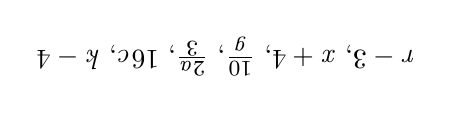
\begin{tikzpicture}
\node [rotate=180] {
$r-3$, $x+4$, $\frac{10}{g}$, $\frac{2a}{3}$, $16c$, $k-4$
};
\end{tikzpicture}
\end{center}

When we translate a word expression into an algebraic expression, it is very important to preserve
the order of operations.

The algebraic expression, $3(x + 2)$, is not equivalent to the algebraic expression, $3x + 2$.

The algebraic expressions on the right represent the word expressions on the left.
The variable n will be used to hold the place of the unknown number.

\begin{center}
\begin{tabularu}{c>{$}c<{$}}
\hline
Word Expression & \text{Algebraic Expression}\\
\hline
four times a number & 4x\\
five times the sum of a number and eight & 5(x + 8) \\
Ana's age in 12 years if her present age is $a$ & a + 12\\
5.2 times the square of the length of the radius & 5.2r^2\\
The sum of two consecutive integers if $r$ is the first integer & r + (r + 1)\\
Thrice the difference of a number and one & 3 (x - 1)\\
Fe's age 9 years ago & f-9\\
A given height subtracted from nine times that height & 9h-h\\
\hline
\end{tabularu}
\end{center}

\yourown{}

\begin{center}
\begin{tabularu}{cc}
\hline \hline
Word Expression & Algebraic Expression\\
\hline
\parbox[t][]{0.5\linewidth}{
\begin{enumerate}
\item The difference of 7 and twice a number $y$
\item Twice the difference of 7 and a number $y$
\item Twice the difference of a number $y$ and 7
\item Rey's age in $h$ years if he is 11 now
\end{enumerate}
}
 & \\
\hline
\end{tabularu}
\end{center}
We are already done with translating phrases into algebraic expressions, next is to complete the
mathematical sentence in order to create an algebraic equation.
\begin{definition}[Algebraic equation]
An \Bold{algebraic equation} has an algebraic expression set equal to a number or another expression, e.g., $3x+2=7$, $3n-7=4n$, and $\dfrac{a}{5}+5=10a-8$.
\end{definition}
The key word for translating complete sentences into an equation is the word “is”. All forms of the
word “is” represent the equal sign in an equation.

In this example, let us express the mathematical sentence into an algebraic equation.
“Five years ago, I was half the age I will be in eight years.”
\begin{quote}
\begin{tabular}{l>{$}l<{$}}
Five years ago & a-5\\
I was half the age & \frac{1}{2}\\
I will be in eight years & a+8\\
\end{tabular}
\end{quote}
So, now we will write this sentence as an algebraic equation.
\begin{equation*}
a-5=\frac{1}{2}(a+8)
\end{equation*}
Let's try one more together.
\begin{example}
\Item Five more than twice a number is three times the difference of that number and two.

\textbf{Solution}: 

Let $n=$ the number.

Five \Underline{more than twice} a number \Underline{is} three \Underline{times} the \Underline{difference} of that number and two.

The mathematical equation is $2n + 5 = 3 (n-2)$.
\end{example}
\yourown{}
\begin{center}
\begin{tabular}{p{0.4\linewidth}c}
\hline \hline
\multicolumn{1}{c}{Sentence} & Equation \\
Thrice the sum of eight and a number is twelve less than that same number
 & \\
Nine years from now, Ana will be four times her age from 5 years ago. & \\
\end{tabular}
\end{center}
\begin{example}
\Item Three consecutive integers sum to 99.

\Solution

Consecutive integers increase by one each time.

Let
\begin{tabular}[t]{@{}>{$}r<{\,$}@{}l}
x = & the first integer\\
x + 1 = & the second integer\\
x + 2 = & the third integer\\
\end{tabular}

We add our three integers and set that equal to 99.
\begin{equation*}
x + (x + 1) + (x + 2) = 99
\end{equation*}
\end{example}
Let’s try one that is a little harder.
\begin{example}
\Item Jessica has Php 3.15 in 25-centavo, 10-centavo, and 5-centavo coins. She has twice as many 5-
centavo coins as 10-centavo coins as and two less 25-centavo than 5-centavo.

\Solution

Let
\begin{tabular}[t]{@{}>{$}r<{\,$}@{}l}
d = & number of 10-centavo\\
2d = & number of 5-centavo\\
2d - 2 = & number of 25-centavo\\
\end{tabular}
\end{example}

\yourown{Translate the following sentences to equations.}
\begin{center}
\begin{tabularu}{p{0.4\linewidth}c}
\hline \hline
\multicolumn{1}{c}{Sentence} & Equation\\
\hline
Three consecutive integers sum to 96. & \\
Ana has Php 2.00 in the denomination of 25-centavo, 10-centavo, and 5-
centavo coins. The number 10-centavo is twice the number of 5-centavo and
the number of 25-centavo is thrice the number of 5-centavo coins. Form an
e2quatiuon representing the total amount of her coins. & \\
\hline
\end{tabularu}
\end{center}
Here is a summary table which lists some key words and phrases that are used to describe common
mathematical operations.
\begin{longtable}{p{0.2\linewidth}p{0.2\linewidth}p{0.3\linewidth}>{$}p{0.125\linewidth}<{$}}
\kill
\caption{Common key words and phrases for mathematical operations}\label{chap5tab:1}\\
\hline \hline
%\endfooter
Operation & Key Word/Phrase & Example & Translation \\
\hline \hline
\endfirsthead
\caption[]{(continued)}\\
\hline \hline
Operation & Key Word/Phrase & Example & Translation \\
\hline \hline
\endhead
\hline
\multicolumn{4}{r}{{Continued on next page}} \\
\endfoot
\hline
\endlastfoot
Addition ($+$) & plus & a number plus two & n+2\\
 & more than & Six more than a number & n+6\\
 & the sum of & The sum of a number and three & n+3\\
 & the total of & the total of five and a number & n+5\\
 & increased by & A number increased buy one & n+1\\
 & added to & Thirteen added to a number & n+13\\
\hline \hline
Subtraction ($-$) & minus & A number minus eight & n-8\\
 & less than & Two less than a number & n-2\\
 & the difference of & The difference of a number and five & n-5\\
 & less & Eleven less number & 11-n\\
 & decreased by & A number decreased by six & n-6\\
 & subtracted by & Three subtracted by a number & 3-n\\
\hline \hline
Multiplication ($\times$) & times & Three times a number & 3n\\
 & the product of & The product of five and a number & 5n\\
 & twice, double  & Twice a number, double a number  & 2n\\
 & multiplied by  & A number multiplied by four 			& 4n\\
 & of						  & Two-fifths of a number 					& \frac{2n}{5}\\
\hline \hline
Division ($\div$) & The quotient of & The quotient of 2 and a number & \frac{2}{n}\\
 & Divided by & Thirty divided by a number & \frac{30}{n}\\
 & The ratio of & The ratio of a number and six & \frac{n}{6}\\
\hline \hline 
Powers ($x^n$) & the square of & The square of a number or number squared & n^2\\
 & the cube of & The cube of a number or number cubed & n^3\\
\hline \hline
Equals ($=$) & equals & Three less than a number equals nine & n-3=9\\
 & is & Two times a number is 14 & 2n=14\\
 & is the same as & Fifteen is the same as thrice a number & 15=3n\\
 & yields & A number added to one yields four & n+1=4\\
 & amounts to & Six less than a number amounts to twenty-four & n-6=24\\
\hline 
\end{longtable}


\section*{SUGGESTED ACTIVITIES}
\subsection*{Activity 1: Translate each word phrase to algebraic expression}
\begin{enumerate}
\item The sum of $n$ and 5. 
\item The product of $x$ and $y$ 
\item Nine more than a number 
\item Twice of a number 
\item Three-fourths of a number 
\item A number decreased by 8 
\item 10 more than the unknown 
\item The quotient of a number and 3 
\item Six more than thrice a number 
\item Five times the sum of a number and 4 
\item The ratio of $x$ and $2y$
\item One less than 9 times a number 
\item Five times a number increased by 4 
\item One more than a number 
\item The product of twice a number and 8 increased by six 
\end{enumerate}
\Answers
\begin{enumerate}
\item $n+5$
\item $xy$
\item $x+9$
\item $2x$
\item $\frac{3x}{4}$
\item $x-8$
\item $x + 10$
\item $\frac{x}{3}$
\item $3x + 6$
\item $5(x +4)$
\item $\frac{x}{2y}$
\item $9x-1$
\item $5x + 4$
\item $x+1$
\item $(2x)(8) + 6$
\end{enumerate}
\subsection*{Activity 2: Translating Exercise}
Write a word phrase for each algebraic expression: (Note: There are many ways in writing a word
phrase for certain algebraic expression)
\begin{enumerate}
\item $\frac{2}{y}$
\item $x + 4$
\item $x-6$
\item $7x + 4$
\item $2x-6$
\item $3(n + 2)$
\item $52-4a$
\item $x^2+2$
\item $\frac{2x+3}{7}$
\item $5-\frac{3}{x}$
\end{enumerate}
\Answers
\begin{enumerate}
\item The quotient of 2 and $y$.
\item A number increased by 4.
\item Six less than a number.
\item Four more than seven times a number.
\item Twice a number less than six.
\item Thrice the sum of n and 2.
\item Fifty-two decreased by four times a number
\item The square of $x$ added to 2.
\item The quotient of twice of $x$ added to 3 and 7.
\item Five decreased by the quotient of 3 and $x$.
\end{enumerate}
\subsection*{Activity 3: Translating Activity 3}
\begin{enumerate}
\item $7x +3 = 17$
\item $4(x + 5) < 20$
\item $(3x)(8) - 7 =31$
\item $x+\frac{x}{3}\ge 16$
\item $8 - 4x = 7$
\item $x + (x + 2) = 14$
\item $\frac{x}{5}-100$
\item $3(x + 9) = 36$
\item $3x + 9 = 36$
\item $2x + 3x = 75$
\end{enumerate}
\Answers
\begin{enumerate}
\item Seven times a number increased by 3 is 17.
\item Four times the sum of a number and five is less than twenty.
\item The product of thrice a number and 8 decreased by 7 is 31.
\item A number increased one-third of itself is greater than or equal to 16.
\item The difference of eight and four time a number is 7.
\item The sum of two consecutive even integers is 14.
\item The quotient of a number and 5 decreased by 15 is 100.
\item Thrice the sum of a number and 9 is 36
\item The sum of thrice a number and 9 is 36.
\item Twice a number added by thrice of same number is 75.
\end{enumerate}
\subsection*{Activity 4: Translating Activity 4}
Give the equation/inequality for the given sentence/situation.
\begin{enumerate}[A.]
\item Number Problems
	\begin{enumerate}
	\item Twice a number increased by 12 is 48.
	\item The difference of twice a number and 5 is 7.
	\item The product of a number and 11 is less than or equal to 165.
	\item Decreasing a number by 25 gives 42.
	\item The larger number is four more than the smaller number. If their sum is 72, form an equation stating their sum.
	\item The sum of two numbers is 92. One number is twelve less than the other. Find numbers. 
	\item The sum of two consecutive integers is sixty-three.
	\item A number added to half of itself is 9. 
	\end{enumerate}
\item Age Problems 
	\begin{enumerate}
	\item Rona's age five years ago was 25. 
	\item Ten less thrice of Fe's age is 58. 
	\item Cora is three years older than Din. If the sum of 
    their ages is 35 years, form an equation representing 
    the sum of their ages. 
	\item Ana is five years older than Jen. If the sum of their 
    ages is 11, form an equation stating the sum of their 
    ages.
	\end{enumerate}
\item Money Problems
	\begin{enumerate}
	\item Fe saves 5-centavo and 10-centavo coins. If she has 28 coins worth Php 2.60, form an equation
representing the total amount of her coins.
	\item Jen has 26 coins in the denomination of 5 centavos and 25 centavo. If the total amount of her coins is Php 3.10, form an equation representing the total amount of her coins.
	\end{enumerate}
\item Investment Problem
	\begin{enumerate}
	\item An amount of Php 10,000 is invested at 3.5\% simple interest for one year. Form an equation representing the interest.
	\item Len invested some money at 3\% and Php 4000 less than that amount at 5\%. The two investments produced a total of Php 200 interest in one year. Form an equation representing the total interest of the two investments.
	\end{enumerate}
\item Mixture Problem
	\begin{enumerate}
	\item A mechanic added 25\mL of water to 125\mL of a 20\% solution of antifreeze in water. Form an equation representing the concentration of antifreeze in the new solution?
	\item A certain amount of water was added to a 50\mL solution of 25\% acid in water. If the resulting mixture has concentration of 10\% acid, form an
equation representing the concentration of the new
mixture.
	\end{enumerate}
\item Uniform Motion Problem
	\begin{enumerate}
	\item Two trains leave from a station at the same time. They travel in opposite directions, one at 62 km/h and the other at 48 km/h. If they are 550 km after certain time, form an equation representing the total distance covered by the two trains.
	\item Two hikers leave on same the place at the same time and travels in opposite direction, one travels 2 kph faster than the other. If they 168 km apart after 4 hours, form an equation representing the total distance covered by the hikers after 4 hours.
	\end{enumerate}
\end{enumerate}
\subsection*{Activity 5: Math BINGO}\label{chap5sec:1}
\subsubsection*{Level 1}
\begin{enumerate}[Step 1.]
\item The participants will have to translate the verbal phrases to mathematical expressions and
randomly place them on their bingo cards.
\item The facilitators will check if everybody has finished accomplishing their bingo cards.
\item The resource person will announce the pattern to be accomplished. There could be more
than 1 winning pattern for higher chances of winning.
\item The resource person will randomly read verbal phrase one at a time and the participants will
mark the corresponding mathematical expression on their bingo card.
\item If a pattern is completed, the participant will just have to “announce”. The facilitator and
resource person will verify the correctness of the bingo card. If there is a wrong entry, the
participant is disqualified and the activity continues. Otherwise, the winner is proclaimed.
\item The game may continue for the other patterns or the game may be restarted for a different
pattern.
\end{enumerate}
\begin{figure}[!h]
\centering
\caption{Bingo Cards for Activity \eqref{chap5sec:1}}
\begin{tabular}{|c|c|c|c|c|c|c|}
\hline
\multicolumn{7}{|c|}{Game 1}\\
\hline
\multicolumn{7}{|c|}{}\\
\cline{2-6}
\hphantom{.} & P & I & S & A & Y & \hphantom{.}\\
\cline{2-6}
 & & &\cellcolor{\bingo} & & & \\ \cline{2-6}
 & & &\cellcolor{\bingo} & & & \\ \cline{2-6}
 & & &\cellcolor{\bingo} & & & \\ \cline{2-6}
 & & &\cellcolor{\bingo} & & & \\ \cline{2-6}
 & & &\cellcolor{\bingo} & & & \\ \cline{2-6}
\multicolumn{7}{|c|}{}\\
\hline
\end{tabular}
\hfil 
\begin{tabular}{|c|c|c|c|c|c|c|}
\hline
\multicolumn{7}{|c|}{Game 1}\\
\hline
\multicolumn{7}{|c|}{}\\
\cline{2-6}
\hphantom{.} & P & I & S & A & Y & \hphantom{.}\\
\cline{2-6}
 &\cellcolor{\bingo} & & & & \cellcolor{\bingo} & \\ \cline{2-6}
 & & & & & & \\ \cline{2-6}
 & & &\cellcolor{\bingo} & & & \\ \cline{2-6}
 & & & & & & \\ \cline{2-6}
 & \cellcolor{\bingo} & & & & \cellcolor{\bingo} & \\ \cline{2-6}
\multicolumn{7}{|c|}{}\\
\hline
\end{tabular}
\hfil 
\begin{tabular}{|c|c|c|c|c|c|c|}
\hline
\multicolumn{7}{|c|}{Game 1}\\
\hline
\multicolumn{7}{|c|}{}\\
\cline{2-6}
\hphantom{.} & P & I & S & A & Y & \hphantom{.}\\
\cline{2-6}
 &\cellcolor{\bingo} & & & & \cellcolor{\bingo} & \\ \cline{2-6}
 & & \cellcolor{\bingo} & & \cellcolor{\bingo} & & \\ \cline{2-6}
 & & &\cellcolor{\bingo} & & & \\ \cline{2-6}
 & & \cellcolor{\bingo} & & \cellcolor{\bingo} & & \\ \cline{2-6}
 & \cellcolor{\bingo} & & & & \cellcolor{\bingo} & \\ \cline{2-6}
\multicolumn{7}{|c|}{}\\
\hline
\end{tabular}
\label{chap5fig:1}
\end{figure}

\begin{center}
\begin{longtable}{p{0.5\linewidth}>{\centering\arraybackslash$}p{0.3\linewidth}<{$}}
\kill
\caption{Questions for \eqref{chap5fig:1}}\label{chap5tab:3}\\
\hline \hline
\parbox[t]{\linewidth}{\centering
Verbal Phrases\\
(In the Bingo Box)
} & 
\parbox[t]{\linewidth}{\centering
Mathematical Expressions\\
(Card Entries)
}\\
\hline \hline
\endfirsthead
\caption[]{(continued)}\\
\hline \hline
\parbox[t]{\linewidth}{\centering
Verbal Phrases\\
(In the Bingo Box)
} & 
\parbox[t]{\linewidth}{\centering
Mathematical Expressions\\
(Card Entries)
}\\
\hline \hline
\endhead

\hline \hline
\multicolumn{2}{r}{{Continued on next page}} \\
\endfoot

\hline \hline
\endlastfoot
a number decreased by seventy-eight & n-78\\
the difference between a number and twenty-seven & n-27\\
the quotient of a number and fifty-three & \frac{n}{53}\\
the sum of four and a number & 4+n\\
the quotient of sixty-five and a number & \frac{65}{n}\\
a number increased by fifty-eight & n+58\\
the difference between thirty-six and a number & 36-n\\
a number added to fifty-six & 56+n\\
seventy-three less than a number & n-73\\
the product of a number and forty-four & 44n\\
a number decreased by thirty-three & n-33\\
twenty-eight times a number & 28n\\
the sum of twenty-three and a number & 23+n\\
the quotient of a number and seventy-nine & \frac{n}{79}\\
the difference between a number and fifty-nine & n-59\\
the sum of a number and thirty-seven & n+37\\
the quotient of sixty-one and a number & \frac{61}{x}\\
a number increased by ninety-three & x+93\\
the product of thirty-two and a number & 32x\\
the product of twenty-five and a number & 25x\\
the difference between a number and eight & x-8\\
nine more than a number & x+9\\
fifty-nine times a number & 59x\\
the quotient of a number and ninety-seven & \frac{x}{97}\\
seventeen times a number & 17x\\
the sum of sixty-one and a number & 61+x\\
a number decreased by eighty-six & x-86\\
the difference between ninety and a number & 90-x\\
eighty-one less than a number & x-81\\
The sum of a number and 3 & x+3\\
The product of a number and 3 & 3x\\
The sum of two numbers & x+y\\
Three times the sum of two numbers & 3(x+y)\\
Three times a number & 3x\\
Three less than a number & x-3\\
A number, less 3 & x-3\\
Three more than a number & x+3\\
A number, plus 3 & x+3\\
The square of a number & x^2\\
The square of three times a number & (3x)^2\\
Three times the square of a number & 3x^2\\
One-third of a number & \frac{x}{3}\\
One less than 3 times a number & 3x-1\\
Two more than 5 times a number & 5x+2\\
The square of the sum of two numbers & (x+y)^2\\
The sum of the squares of two numbers & x^2+y^2\\
\hline
\end{longtable}
\end{center}

\subsection*{Activity 6: Bingo Activity 2}\label{chap5sec:2}
\begin{figure}[!ht]
\centering
\caption{Bingo Cards for Activity 2}
\begin{tabular}{|c|c|c|c|c|c|}
\hline
\multicolumn{6}{|c|}{|Game 4|}\\
\cline{2-5}
 & M & A & T & H & \\ \cline{2-5}
 & & & & & \\ \cline{2-5}
 & & \cellcolor{\bingo} & \cellcolor{\bingo} & & \\ \cline{2-5}
 & & \cellcolor{\bingo} & \cellcolor{\bingo} & & \\ \cline{2-5}
 & & & & & \\ \cline{2-5}
\multicolumn{6}{|c|}{}\\
\hline
\end{tabular}
\hfil 
\begin{tabular}{|c|c|c|c|c|c|}
\hline
\multicolumn{6}{|c|}{|Game 5|}\\
\cline{2-5}
 & M & A & T & H & \\ \cline{2-5}
 & &\cellcolor{\bingo} & \cellcolor{\bingo} & & \\ \cline{2-5}
 &\cellcolor{\bingo} & & & \cellcolor{\bingo} & \\ \cline{2-5}
 & \cellcolor{\bingo} & & & \cellcolor{\bingo} & \\ \cline{2-5}
 & & \cellcolor{\bingo} & \cellcolor{\bingo} & & \\ \cline{2-5}
\multicolumn{6}{|c|}{}\\
\hline
\end{tabular}
\label{chap5fig:2}
\end{figure}
Follow the same procedures in Activity \eqref{chap5sec:1}.

\begin{center}
\begin{longtable}{p{0.5\linewidth}>{\centering\arraybackslash$}p{0.3\linewidth}<{$}}
\kill
\caption{Questions for \eqref{chap5fig:2}}\label{chap5tab:4}\\
\hline \hline
\parbox[t]{\linewidth}{\centering
Verbal Phrases\\
(In the Bingo Box)
} & 
\parbox[t]{\linewidth}{\centering
Mathematical Expressions\\
(Card Entries)
}\\
\hline \hline
\endfirsthead
\caption[]{(continued)}\\
\hline \hline
\parbox[t]{\linewidth}{\centering
Verbal Phrases\\
(In the Bingo Box)
} & 
\parbox[t]{\linewidth}{\centering
Mathematical Expressions\\
(Card Entries)
}\\
\hline \hline
\endhead

\hline \hline
\multicolumn{2}{r}{{Continued on next page}} \\
\endfoot

\hline \hline
\endlastfoot
A number increased by nine is fifteen. & \\
Twice a number is eighteen. & \\ \hline
Four less than a number is twenty. & \\ \hline
A number divided by six is eight. & \\ \hline
Twice a number, decreased by twenty-nine, is seven. & \\ \hline
Thirty-two is twice a number increased by eight. & \\ \hline
The quotient of fifty and five more than a number is ten. & \\ \hline
Twelve is sixteen less than four times a number. & \\ \hline
Eleni is x years old. In thirteen years she will be twenty-four years old. & \\ \hline
Each piece of candy costs 25 cents. The price of h pieces of candy is & \\ \hline
Suzanne made a withdrawal of d dollars from her savings account. Her old balance was \$350, and her new balance
is & \\ \hline
A large pizza pie with 15 slices is shared among p students so that each student's share is 3 slices. & \\ \hline
Lorene has some nickels, twice as many dimes as nickels, and half as many quarters as nickels. All total she has 77 coins. & \\ \hline
Jack is 25 years younger than his mother. Together, their ages add up to 89. & \\ \hline
Cucumbers cost 15\textcent{} each and tomatoes costs 9\textcent{} each. Mom buys six more tomatoes than cucumbers. Her total bill is \$1.26. & \\ \hline
Marie bought 12 fruits, of which there were x apples, five fewer oranges than apples, and one pineapple. & \\ \hline
Tara is twice as old as Gwen. Their sister, Amy, is 5 years older than Gwen. If the sum of their ages is 29 years, find each of their ages. & \\ \hline
Carol is 25 years older than her cousin Amanda. Cousin Bill is 3 times as old as Amanda. The sum of their ages is 90. Find each of their ages. & \\ \hline
Derrick is 5 less than twice as old as Brandon. The sum of their ages is 43. How old are Derrick and Brandon? & \\ \hline
Beth’s mom is 6 times older than Beth. Beth’s dad is 7 years older than Beth’s mom. The sum of their ages is 72. How
old are each of them? & \\ \hline
Ruby is 2 years more than three times as old as her son, Raul. If the difference between their ages is 26, how old are Ruby and Raul? & \\ \hline
Sam is ten less than 3 times as old as Alex. If the difference between their ages is 28, how old is Sam and Alex. & \\ \hline
Eileen is 6 years older than Karen. John is three times as old as Karen. The sum of their ages is 56. How old are Eileen, Karen and John? & \\ \hline
Taylor is 18 years younger than Jim. Andrew is twice as old as Taylor. The sum of their ages is 26. How old are Taylor, Jim and Andrew? & \\ \hline
Jick is 3 years less than four times as old as Jall. If the difference between their ages is 72, how old are Jick and Jall? & \\ \hline
Rufio is 15 years younger than Rafe. Rafe is four times older than Raquel. If the sum of their ages is 48 then how old are they? & \\ \hline
Robert and Roberta are twins. The product of their ages is 196. & \\ \hline
\hline
\end{longtable}
\end{center}
\printbibliography[keyword=Module5,heading=subbibliography,title={REFERENCES}]
\chapter[SOLVING LINEAR EQUATIONS AND LINEAR INEQUALITIES]{SOLVING\\ LINEAR EQUATIONS AND\\ LINEAR INEQUALITIES}
\section*{INTRODUCTION}
This section covers equalities and inequalities in one variable (also known as linear equations
and linear inequalities). Equations and inequalities are relations between two quantities. Many real-life situations can be modeled by equations and inequalities. Learning how to solve these
mathematical models enables one to use mathematical solutions to answer real-world problems.
\section*{OBJECTIVES}
\begin{enumerate}
\item Differentiate equations from inequalities.
\item Find the solution of an equation and inequality involving one variable
\begin{enumerate}
	\item from a given replacement set;
	\item intuitively by guess and check;
	\item by algebraic procedures (applying the properties of equalities and inequalities); and/or
	\item by graphing.
\end{enumerate}
\item Check a solution of an equation and inequality.
\item Solve problems involving equations (separate module) and inequalities.
\end{enumerate}
\section*{DISCUSSION}
The mathematical sentence “$4 + 3 = 7$” is true while “$3 > 4$” is false. On the other hand, the
sentences “$x - 3 = 5$” and “$x + 4 > 1$” cannot be determined as true or false until we have a
replacement for the variable $x$. The sentences “$x - 3 = 5$” and “$x + 4 > 1$” are examples of \Bold{open
sentences}. An open sentence of the first degree in one variable can either be an \Bold{equation} or an
\Bold{inequality}. First degree equations and inequalities in one variable are known as \Bold{linear equations} or
\Bold{linear inequalities}.

An \Bold{equation} is a statement that expresses the equality of two mathematical expressions. A lunear
equation is of the form $\mathbf{ax + b = c}$ where $a$, $b$ and $c$ are any real numbers. To solve an equation is to
find a value of the variable that makes the equation true. This value which can replace the variable in
the equation is called a \Bold{root} or a \Bold{solution} of the equation. For example, 2 is a solution of the
equation $2x - 3 = 1$ because when 2 is substituted to $x$, $2(2) - 3 = 1$ which may be simplified to the
true statement $1 = 1$.

The \Bold{replacement set} or \Bold{domain} is the set of possible values that can be used in place of the variable
in an open sentence. A collection of all solutions or all elements of the replacement set of an
equation is called the \Bold{solution set} of the equation. Equations having the same solution are said to be
\Bold{equivalent equations}.

Solving equations and inequalities can be done in four ways: a) from a given \Bold{replacement set};
b) \Bold{guess and check}--one guesses and substitutes values into the equation then check if a true
statement will result; c) \Bold{algebraic procedures}; and d) \Bold{graphing}. Since there is only one or unique
solution of an equation, the graphical method (graphical method) is more emphasized in solving
inequalities.

\begin{property}[frametitle={Properties of Equality}]
\begin{itemize}
\item \Bold{Reflexivity}: For any real number $a$, $a
= a$; that is, anything is equal to itself.
\item \Bold{Symmetry}: For any real numbers $a$ and $b$, if $a=b$, then $b=a$.
\item \Bold{Transitivity}: For any real numbers $a$, $b$ and $c$, if $a=b$ and $b=c$, then $a=c$.
\item \Bold{Adition Property of Equality} \Bold{(APE)}: Any real number added to both sides of an
equation does not change the nature of the equation. That is, if $a$, $b$ and $c$ are real numbers, and $a = b$, then $a + c = b + c$.
\item \Bold{Multiplication Property of Equality} \Bold{MPE}: ny real number multiplied to both sides
of an equation does not change the nature of the equation. That is, if $a$, $b$ and $c$ are real numbers, and $a = b$, then $ac = b c$.
\end{itemize}
\end{property}
\begin{example}
\Item Find the solution set of $2 - 5z = 7$. The replacement set is $\{-1, 0, 1\}$. \hfill \textbf{(From a given replacement set)}

\Solution

\begin{tabularu}{>{$}l<{$}>{$}l<{$}>{$}l<{$}}
\text{Replace $z$ with $-1$}. & \text{Replace $z$ with $0$}. & \text{Replace $z$ with $1$}.\\
2-5z = 7 & 2-5z = 7 & 2-5z = 7\\
2-5(-1) = 7? & 2-5(0) = 7? & 2-5(1) = 7?\\
2+5=7? & 2-0=7? & 2-5=7?\\
7=7\quad \mathbf{True} & 2=7\quad \mathbf{False} & -3 = 7\quad \mathbf{False}\\
\end{tabularu}

The value of $-1$ for $z$ makes $2 - 5z = 7$ true. The solution set is $\{-1\}$.

When no number from the replacement set makes the open sentence true, then the solution set is null.

\Item Check whether 0, 1, 4 and 6 are solutions of $3x-15 = 3.$ \hfill \textbf{(By guess and check.)}

\Solution

\begin{tabularu}{>{$}l<{$}>{$}l<{$}l}
x=0: & 3(0)-15=3? & No, 0 is not a solution of the given equation because $-15\neq 3$.\\
x=1: & 3 (1)-15 = 3? & No, 1 is not a solution because $-12\neq3$\\
x=4: & 3 (4)-15 = 3? & No, 4 is not a solution because $-3\neq 3$\\
x=6: & 3 (6)-15 = 3? & Yes, 6 is a solution of the equation because $3 = 3$.
\end{tabularu}
\Item Solve the following equations: \hfill \textbf{(By algebraic procedure)}
	\begin{enumerate}[1.]
	\item $2x+1=2x+3$
	
	Since the terms $2x$ of the equation cancels out after adding $-2x$ on both sides, the equation simplifies to $1 = 3$, which is a false statement. This equation is an example of a \Bold{contradiction}, an equation that cannot be true for any value of the variable. \underline{Its solution set is the null set}.

	\item $2x + 1 = x + 3$
	
	Upon solving, the value $x = 2$ makes the equation true. This linear equation is an example of a \Bold{conditional equation}, an equation which is true only for a particular value of the variable. For linear conditional equations, exactly one real number will satisfy it. \underline{Therefore, its solution set is a unit set or a singleton (a one-element set)}.
	
	\item $2x + 1 = 2x + 1$
	
	Since the terms $2x$ of the equation cancels out after adding $-2x$ on both sides, the equation simplifies to $1 = 1$, which is a true statement. This equation is an example of an identity, an equation that is true for any value of the variable. Its solution set is the set of real numbers.
	\end{enumerate}
\end{example}
\subsection*{Exercises}
\begin{enumerate}[I.]
\item Find the solution set of each equation if the replacement set is $\{-2, 0, 2\}$.
	\begin{enumerate}[1.]
	\item $x+3=1$
	\item $5-2y=1$
	\item $x=-x$
	\item $\frac{3y}{2}+\frac{1}{2}=2$
	\item $4t-4(t-3) = 12$
	\item $-2(z-5) = 8-2z$
	\end{enumerate}
	\rotatedbox{%
	\begin{inparaenum}[1.]
	\item $\{-2\}$
	\item $\{2\}$
	\item $\{0\}$
	\item $\{\}$
	\item $\{-2,0,2\}$
	\item $\{\}$
	\end{inparaenum}		
	}

\item Find the solution set of the following equations and classify if it is a contradiction, conditional or identity.
	\begin{enumerate}[1.]
	\item $x+3=1$
	\item $5-2y=1$
	\item $x=-x$
	\item $\frac{3y}{2}+\frac{1}{2}=2$
	\item $4t-4(t-3) = 12$
	\item $-2(z-5) = 8-2z$
	\end{enumerate}
	\rotatedbox{%
	\begin{inparaenum}[1.]
	\item $\{-2\}$ conditional
	\item $\{2\}$ conditional
	\item $\{0\}$ conditional
	\item $\{1\}$ conditional
	\item $\mathbb{R}$ identity
	\item $\{\}$ contradiction
	\end{inparaenum}
	}

\item Give the solution sets of the following equations.
	\begin{enumerate}[1.]
	\item $3x +4 = 2(x - 6) + (x + 16)$
	\item $2.3 x-2(x + 1) = 0.7$
	\item $5x + 7 = 7x + 5 – (2x + 2)$\\
	\item $8(3p-1)-5(3p + 2) = 3(2p-1)$
	\item $\frac{x+1}{3}-\frac{x+2}{3}=\frac{x}{2}$
	\item $2(x + 1) + 7(x-1) = 3(x + 1) + 6(x-1)$
	\end{enumerate}
	\rotatedbox{
	\begin{inparaenum}[1.]
	\item $\mathbb{R}$
	\item $\{9\}$
	\item $\{\}$
	\item $\{5\}$
	\item $\{-\frac{2}{3}\}$
	\item $\{\}$
	\end{inparaenum}		
	}
\end{enumerate}

\subsection*{GRAPHING EQUATIONS AND INEQUALITIES}
A \Bold{number line} represents the order of real numbers. Also, real numbers can be represented as points in the number line. On the number line shown in Figure \eqref{chap6fig:1}, point $A$ is the graph of $-3$.
\begin{figure}[!h]
\centering
\caption{A point on the number line.}
\tikz [scale=0.8] {
\draw [<->] (-8.5,0) -- (6.5,0);
\foreach \x in {-8,-7,-6,...,4,5,6}
	\draw (\x,2pt) -- (\x,-2pt) node [below] {$\x$};
\node [above] at (-3,0) {$A$};
\fill [blue,opacity=.5] (-3,0) circle (3pt);
}
\label{chap6fig:1}
\end{figure}

If a number is found on the left of another number on the number line, it is always less than the number on its right. For example, $-5$ is less than $-4$ because $-5$ is on the left of $-4$.

\subsection*{Exercises}
Graph these numbers on the number line.

\begin{inparaenum}
\item 2.5 \hfil \item $-1\frac{1}{2}$ \hfil \item $\frac{5}{4}$ \hfil \item $-3\frac{2}{3}$
\end{inparaenum}

Draw the graph of the following.

\begin{inparaenum}
\item $x<4$ \hfil \item $x\ge\frac{1}{2}$ \hfil \item $x\neq 1$ \hfil \item $x\le \frac{1}{3}$
\end{inparaenum}

\subsection*{INEQUALITIES IN ONE VARIABLE}
Another type of an open sentence is an inequality. A linear inequality is of the form $ax + b < c$ or
$ax + b > c$ or $ax + b\le c$ or $ax + b \ge c$ where $a$, $b$ and $c$ are real numbers. Take note of the inequality symbols and their meanings.

\begin{table}[!h]
\centering
\caption{Inequality symbols and their meaning}
\begin{tabular}{>{$}c<{$}l}
\hline \hline
\text{Inequality Symbol} & Meaning\\
< & less than\\
> & greater than\\
\le & less than or equal to\\
\ge & greater than or equal to\\
\neq & not equal to\\
\hline 
\end{tabular}
\label{chap6tab:1}\eqref{chap6tab:1}
\end{table}

A solution of an inequality is a number that satisfies the inequality statement when it is substituted. For example, 1 is a solution of $x + 1 < 6$ because $2 < 6$ is a true statement. But 1 is not the only solution to $x + 1 < 6$. We can have 2, 3, 4, 5 or 2.2 because all these make the
inequality statement true. We can write the \Ital{solution} as $x < 5$.

\begin{property}[frametitle={Trichotomy Property}]
If $a$ and $b$ are real numbers, then one and only one of the following is true:
\begin{itemize}
\item \begin{tabular}[b]{cc}
$a>b$ & \tikz [baseline=(current bounding box.east)] {
\draw [xscale=-0.5,->] (0,0) -- (1,0);
\draw  (0,0) -- (1,0);
\draw [xscale=1.5,->] (0,0) -- (1,0);
\foreach \x/\xtext in {0/a,1/b}
	\draw (\x,2pt) -- (\x,-2pt) node [below] {$\xtext$};
} \\
\end{tabular}
\item \begin{tabular}[b]{cc}
$a=b$ & \tikz [baseline=(current bounding box.east)] {
\draw [xscale=-0.5,->] (0,0) -- (1,0);
\draw  (0,0) -- (1,0);
\draw [xscale=1.5,->] (0,0) -- (1,0);
\draw (0.5,-2pt) -- (0.5,2pt);
\node [below] (0,0) {$b$};
\node [above] (0,0) {$a$};
} \\
\end{tabular}
\item \begin{tabular}[b]{cc}
$a>b$ & \tikz [baseline=(current bounding box.east)] {
\draw [xscale=-0.5,->] (0,0) -- (1,0);
\draw  (0,0) -- (1,0);
\draw [xscale=1.5,->] (0,0) -- (1,0);
\foreach \x/\xtext in {0/b,1/a}
	\draw (\x,2pt) -- (\x,-2pt) node [below] {$\xtext$};
} \\
\end{tabular}
\end{itemize}
\end{property}
Solving inequalities follows the same procedure as solving equations. The same properties hold except for the multiplication property. A negative real number multiplied to both sides of an inequality \Ital{reverses} the \Ital{direction} of the inequality. Why is this so?

Let's take a look. Try multiplying or dividing the statement below by a negative number, say $-2$.
\begin{align*}
2&<3 && \text{true statement}\\
-2(2) &\overset{?}{<}-2(3) && \text{multiply by $-2$}\\
-4&\overset{?}{-6} && \text{Is this statement true?}\\
 & && \text{\textbf{No, $\mathbf{-4}$ is greater than $\mathbf{-6}$}}\\
-4 &\overset{\checkmark}{>}-6 && \text{To make the statement true, reverse the sign.}
\end{align*}
Let’s summarize the properties of inequality.
\begin{property}[frametitle={Properties of Inequality}]
The following \Bold{properties of inequality} hold for any real numbers $a$, $b$ and $c$.
\begin{itemize}
\item \Bold{Transitivity}: If $a<b$ and $b<c$, then $a<c$.
\item \Bold{Addition Property of Inequality} (\Bold{API}): If $a<b$, then $a+c<b+c$.
\item \Bold{Multiplication Property of Inequality} (\Bold{MPI}): If $a<b$ and $c>0$ ($c<0$), then $ac<bc$ ($ac>bc$).
\end{itemize}
\end{property}
The solution of inequalities is more concretized when it is simultaneously presented with a graph.

The following are graphing symbols that will be used in solving inequalities.
\begin{property}[frametitle={Graphing Symbols}]
\begin{tabular}[t]{lp{0.7\linewidth}}
\tikz [baseline=(current bounding box.east),very thick,>=stealth'] {
\node (a) [circle, minimum width=6pt,draw,inner sep=0pt] {};
\draw [->] (a) -- +(1,0);
} & 
  greater than (the open circle indicates that this is \Ital{not} equal to the number graphed)\\
\tikz [baseline=(current bounding box.east),very thick,>=stealth'] {
\node (a) [circle, minimum width=6pt,draw,fill,inner sep=0pt] {};
\draw [->] (a) -- +(1,0);
} & greater than or equal to (the closed circle indicates that this is equal to the number graphed)\\
\tikz [baseline=(current bounding box.east),very thick,>=stealth'] {
\node (a) [circle, minimum width=6pt,draw,inner sep=0pt] {};
\draw [->] (a) -- +(-1,0);
} & less than\\
\tikz [baseline=(current bounding box.east),very thick,>=stealth'] {
\node (a) [circle, minimum width=6pt,draw,fill,inner sep=0pt] {};
\draw [->] (a) -- +(-1,0);
} & less than or equal to\\
\end{tabular} 
\end{property}
\begin{example}[I.]
\Item Solve the following inequalities then graph the solution set on a number line:
	\begin{enumerate}[1.]
	\item $3x + 2<2$
	
	\Solution
	{\setlength{\abovedisplayskip}{0pt}
	\begin{align*}
	3x+2+(-2)&<2+(-2) && \text{API (add $-2$ to both sides)}\\
	3x+0&<0 && \text{Additive inverse property}\\
	3x&<0 && \text{Additive identity property}\\
	\Bigl(\frac{1}{3}\Bigr)3x&<\Bigl(\frac{1}{3}\Bigr)(0) && \text{MPI}\\
	x&<0 && \text{Zero property}
	\end{align*}}
	We can give the solution set as $x<3$ or as $\{x\vert x<3\}$ and we can graph this as in \eqref{chap6fig:2}.
	\begin{figure}[!h]
	\centering
	\caption{Solution of $x<3$}
	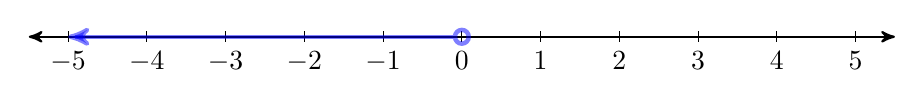
\begin{tikzpicture}[>=stealth']
	\foreach \x in {-5,-4,...,4,5}
		\draw (\x,2pt) -- (\x,-2pt) node [below] {$\x$};
	\draw [<->, thick] (-5.5,0) -- (5.5,0);
	\node (a) [circle, ultra thick, inner sep=0pt, blue, opacity=0.5, text width=5pt, draw] {};
	\draw [->, ultra thick,blue,opacity=0.5] (a) -- +(-5,0);
	\end{tikzpicture}
	\label{chap6fig:2}
	\end{figure}
	The open circle on 0 indicates that 0 is not part of the solution set.

\CHECK: Take a test value on the interval, say $x = -1$.
\begin{align*}
3x+2&<2\\
3(-1)+2&\overset{?}{<}2\\
-3+2&\overset{?}{<}2\\
-1&\overset{\checkmark}{<}2
\end{align*}

\item $12-4(x-5)$

\Solution
\begin{align*}
12 &\ge -4x+20 && \text{Distributive Property}\\
12-20 & \ge -4x+20-20 && \text{API}\\
-8 & \ge -4x && \text{Simplify}\\
\Bigl(\frac{1}{-4}\Bigr) &\le \Bigl(\frac{1}{-4}\Bigr)(-4x) && \text{MPI}\\
2 &\le x && \text{Multiplicative inverse property}\\
x &\ge 2 && \text{It's easier when the variable comes first.}
\end{align*}
\textbf{Solution set:} $\{x\vert x\ge 2\}$
\begin{figure}[!h]
\centering
\caption{Notice the closed interval on $x=2$. This indicates that 2 is part of the solution set.}
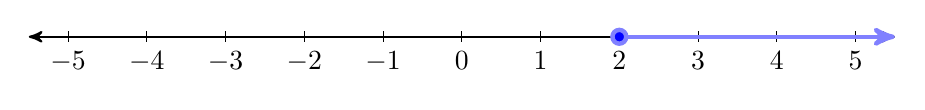
\begin{tikzpicture}[>=stealth']
	\foreach \x in {-5,-4,...,4,5}
		\draw (\x,2pt) -- (\x,-2pt) node [below] {$\x$};
	\draw [<->, thick] (-5.5,0) -- (5.5,0);
	\node (a) at (2,0) [circle, ultra thick, inner sep=0pt, blue!50, text width=5pt, draw,fill=blue] {};
	\draw [->, ultra thick,blue!50!white] (a) -- (5.5,0);
\end{tikzpicture}
\label{chap6fig:3}
\end{figure}

\CHECK{} Test value: $x=3$
\begin{align*}
12&\overset{?}{\ge}-4(x-5)\\
12&\overset{?}{\ge}-4(3-5)\\
12&\overset{?}{\ge}-4(-2)\\
12&\overset{\checkmark}{\ge}8
\end{align*}
	\end{enumerate}
\end{example}
\subsection*{APPLICATION OF LINEAR INEQUALITIES}
The skill of being able to translate sentences into mathematical symbols is a must in successful
problem solving. Some of the \Bold{inequality key words} are the following.
\begin{property}[frametitle={Inequality key words}]
\begin{center}
\begin{tabular}{ll}
at least	 \tikzmark{a1} & \tikzmark{a2} greater than or equal to\\
no more than \tikzmark{b1} & \tikzmark{b2}	less than or equal to\\
more than \tikzmark{c1} & \tikzmark{c2}	greater than\\
at most \tikzmark{d1} & \tikzmark{d2} less than or equal to\\
\end{tabular}
\end{center}
\end{property}
\begin{tikzpicture}[remember picture, overlay,ultra thick, blue,yshift=1pt]
\draw [->] (a1.north) -- (a2.north);
\draw [->] (b1.north) -- (b2.north);
\draw [->] (c1.north) -- (c2.north);
\draw [->] (d1.north) -- (d2.north);
\end{tikzpicture}
\begin{example}
\Item Taxi operators in Metro Manila charges \textpeso40 as flag down rate, in addition to \textpeso3.50 per 300
meters or 2 minutes of waiting time. Macy has no more than \textpeso250 to spend on a ride.
	\begin{itemize}
	\item Write an inequality that represents Macy's situation, assuming that there was no instance that the taxi stopped moving (no waiting time).
	\item How many kilometers can Macy travel without exceeding her limit?
	
	\Solution: Let $k=$ number of \km{} Macy can travel without exceeding her limit
	\begin{equation*}
	\frac{\textpeso 3.50}{300\m}\times \frac{100\m}{1\km}=\textpeso\frac{35}{3}/\km
	\end{equation*}
	\begin{center}
	\begin{tabular}{YYYYY}
	\Tikzmark{e1}{$\dfrac{\mathrm{P}35}{3}$} &  \Tikzmark{e2}{$+$} & \Tikzmark{e3}{40} & \Tikzmark{e4}{$\le$} & \Tikzmark{e5}{250}\\
	& & & & \\
	& & & & \\
	\Tikzmark{f1}{P 35/3 per \km} &  & \Tikzmark{f3}{flag down rate} & \Tikzmark{f4}{no more than} & \Tikzmark{f5}{amount to spend}\\
	\end{tabular}
	\begin{tikzpicture}[remember picture, overlay,ultra thick, blue,yshift=1pt,>=stealth']
\draw [->] (e1.south) -- (f1.north);
\draw [->] (e3.south) -- (f3.north);
\draw [->] (e4.south) -- (f4.north);
\draw [->] (e5.south) -- (f5.north);
\end{tikzpicture}
	\end{center}
	\begin{equation*}
	\frac{35}{3}k\le 250-40\iff \frac{35}{3}k\le 210 \iff 35k\le 630 \iff k\le 18\km
	\end{equation*}
	Thus, Macy cannot go beyond 18 \km.
	\end{itemize}
\Item Salyn has P20,000 in a savings account at the beginning of the year. She wants to have at least
P14,000 in her account by the end of the summer. She withdraws P 500 every week for
miscellaneous expenses.
	\begin{itemize}
	\item Write an inequality that represents Salyn's situation.
	\item How many weeks can Salyn withdraw money from her account?
	
	\Solution{}
	
	Let $w =$ number of weeks Salyn can withdraw money from her savings account
\begin{center}
	\begin{tabular}{YYYY@{}Y@{}}
	\Tikzmark{g1}{20,000} &  \Tikzmark{g2}{$-$} & \Tikzmark{g3}{$500w$} & \Tikzmark{g4}{$\ge$} & \Tikzmark{g5}{14,000}\\
	& & & & \\
	& & & & \\
	& & & & \\
	\Tikzmark{h1}{} & \Tikzmark{h2}{withdraw} & \Tikzmark{h3}{} & \Tikzmark{h4}{at least} & \tikz [remember picture, overlay] \node (h5) [text width=\linewidth, align=center] {desired amount left at the end of summer};\\
	\end{tabular}
	\begin{tikzpicture}[remember picture, overlay,ultra thick, blue,yshift=1pt,>=stealth']
\draw [->] (g2.south) -- (h2.north);
\draw [->] (g4.south) -- (h4.north);
\draw [->] (g5.south) -- (h5.north);
\end{tikzpicture}
	\end{center}
	\begin{align*}
	-500w&\ge 14,000-20,000\\
	-500w&\ge -6,000\\
	\frac{-500w}{-500}&\ge \frac{-6,000}{-500} && \text{division by a negative number}\\
	w&\le 12\; \text{weeks}
	\end{align*}
	Thus, Salyn has a maximum of 12 weeks to withdraw P500 weekly.
	\end{itemize}
\Item Owen wants to order USBs on the Internet. Each USB costs P250.00 and shipping for the entire
order is P200.00. Owen has at most P5,300 to spend.
	\begin{itemize}
	\item Write an inequality that represents Owen's situation.
	\item How many USB's can Owen order with her P5,300?

	\Solution: Let $u =$ number of USBs that Owen can buy
	
	
	\begin{tabular}{YYYYY}
	\Tikzmark{i1}{250u} &  \Tikzmark{i2}{$+$} & \Tikzmark{i3}{200} & \Tikzmark{i4}{$\le$} & \Tikzmark{i5}{5,300}\\
	& & & & \\
	& & & & \\
	& & & & \\
  & & & \Tikzmark{j4}{at most} & \\
	\end{tabular}
	\begin{tikzpicture}[remember picture, overlay,ultra thick, blue,yshift=1pt,>=stealth']
\draw [->] (i4.south) -- (j4.north);
\end{tikzpicture}
	\begin{align*}
	250u&\le 5,100\\
	\frac{250u}{250} & \le \frac{5,100}{250}\\
	\therefore u & \le 20.4
	\end{align*}
	So, Owen can order a maximum of 20 USB's.
	\end{itemize}
\end{example}
\subsection*{Enrichment Lesson: Step-by-step Solving using the Properties of Real Numbers}
Solve $4x-3=25$

\Solution:

\begin{align*}
(4x - 3)+ 3 &= 25 + 3  && \text{Addition Property of Equality}\\
(4x + -3) + 3 &= 25 + 3 && \text{Definition of Subtraction}\\
4x + (-3 + 3) &= 25 + 3 && \text{Commutative Property of Addition}\\
4x + 0 &= 25 + 3 && \text{Inverse Property of Addition}\\
4x &= 25 + 3 && \text{Identity Property of Addition}\\
4x &= 28 && \text{Addition Fact}\\
(4x)\frac{1}{4}&=(29) \frac{1}{4} && \text{Multiplication Property of Equality}\\
(4x)\frac{1}{4}&=7 && \text{Multiplication Fact}\\
\frac{1}{4}(4x)&=7 && \text{Commutative Property of Multiplication}\\
\Bigl( \frac{1}{4}\cdot 4\Bigr)x&=7 && \text{Associative Property of Multiplication}\\
1\cdot x&=7 && \text{Inverse Property of Multiplication}\\
x&=7 && \text{Identity Property of Multiplication}
\end{align*}
\CHECK
\begin{align*}
4 (7) - 3 &\overset{?}{=}25\\
28 - 3 &\overset{?}{=}25\\
25 & \overset{\checkmark}{=}25
\end{align*}
Therefore, $x=7$ is a root or solution of the given equation.
\begin{exercise}
\Item Solve $6(2x-\frac{1}{2})+15=-3(x+1)$ using the procedure above.

\end{exercise}

\printbibliography[keyword=Module6,heading=subbibliography,title={REFERENCES}]
\chapter[SOLVING WORD PROBLEMS USING\\ BLOCK MODEL]{SOLVING WORD PROBLEMS USING\\ BLOCK MODEL}
\section*{INTRODUCTION}
This module is designed to present an alternative method in solving word problems using an
approach that has been used by Singaporean students. For the most part, this module will discuss a
few examples on how this method is applied. After the method has been discussed, the participants
will design their own problems using the block model and present their output to the other
participants.
\section*{OBJECTIVES}
After completing this module, the participant should be able to:
\begin{enumerate}
\item Analyze and solve a given word problem using the block model;
\item Design word problems using the block model.
\end{enumerate}
\section*{DISCUSSION}
During the early 1980s, primary pupils in Singapore were taught basic skills and processes in
problem solving as well as one heuristic which uses “drawing a diagram” to be able to answer the
problem. This method, which was introduced by Dr. Kho Tek Hong and his team, has been used to
solve many challenging arithmetic word problems as well as questions that were designed for
secondary students. In using this method, students draw bars or rectangles in representing the given
problem, and from these representations they analyze what is/are given then solve the problem.
Let us consider the following examples:
\begin{example}
\Item A piece of wire is cut into 3 pieces in the ratio 2:3:5. If the longest piece is longer than the middle piece by 8 cm, find the length of the wire.

From this problem, we can represent the three pieces of wire using bars or rectangles that are of the same dimensions using the ratio 2:3:5, such as

\begin{tabular}{ll}
\tikz [xscale=1.5] {
\foreach \x in {0,1}
	\draw (\x,0) rectangle +(1,1);
} & (shortest piece)\\
\tikz [xscale=1.5] {
\foreach \x in {0,1,2}
	\draw (\x,0) rectangle +(1,1);
} & (middle piece)\\
\tikz [xscale=1.5] {
\foreach \x in {0,1,...,4}
	\draw (\x,0) rectangle +(1,1);
} & (longest piece)\\
\end{tabular}

Notice that from the given problem, it was stated that the longest piece is longer than the middle
piece by 8 cm.

\begin{tabular}{ll}
\tikz [xscale=1.5] {
\foreach \x in {0,1,...,4}
	\draw (\x,0) rectangle +(1,1);
	\draw [decoration={brace,amplitude=5pt},decorate] (5,0) -- (3,0) node [below,pos=0.5,yshift=-5pt] {8 cm};
} & (longest piece)\\
  & \\
  & \\
\tikz [xscale=1.5] {
\foreach \x in {0,1,2}
	\draw (\x,0) rectangle +(1,1);
} & (longest piece)\\
\end{tabular}

This implies that the two bars, which are 8 cm long, have a length of 4 cm each. This means that the shortest piece has a length of 8$\cm$, the middle piece is 12$\cm$ (3 bars $\times$ 4 $\cm$), and the longest piece is 20 $\cm$ (5 bars $\times$ 4$\cm$). Therefore, the length of the wire is $8 \cm + 12 \cm + 20 \cm = 40 \cm$.

\Item The difference of two numbers is 38. One number is only one-third of the other. What are the two numbers?

\Solution{}

\begin{tabular}[b]{ll}
\tikz [xscale=1.5] {
\draw (1,0) rectangle +(1,1);
} & ($1^{st}$ number)\\
  & \\
\tikz [xscale=1.5] {
\foreach \x in {0,1,2}
	\draw (\x,0) rectangle +(1,1);
} & ($2^{nd}$ number)\\
\end{tabular}

It is given that their difference is 38.

\begin{tabular}[b]{ll}
\tikz [xscale=1.5] {
\draw (1,0) rectangle +(1,1);
} & ($1^{st}$ number)\\
  & \\
\tikz [xscale=1.5] {
\foreach \x in {0,1,2}
	\draw (\x,0) rectangle +(1,1);
	\draw [decoration={brace,amplitude=5pt},decorate] (3,0) -- (1,0) node [below,pos=0.5,yshift=-5pt] {38 cm};
} & ($2^{nd}$ number)\\
\end{tabular}

This means that the two bars of the $2^{nd}$ number are worth 38, which implies that each bar is worth 19. Therefore the first number is 19 and the second number is 57 (i.e., $3\times 19$).

\Item Mila spent 1/5 of her money on a pair of shoes and 2/5 of the remainder on a dress. She had
Php 768 left. How much money did she have at first?

From this problem, we can represent Mila's money at first and part of this money that she spent for
the pair of shoes.

\begin{tabular}{ll}
\tikz [xscale=1.5] {
\foreach \x in {0,1,2,3,4}
	\draw (\x,0) rectangle +(1,1);
	\draw [decoration={brace,amplitude=5pt},decorate] (1,0) -- (0,0) node [below,pos=0.5,yshift=-5pt,text width=3cm,align=center] {money spent for the pair of shoes};
} & (money at first)\\
\end{tabular}

After buying the pair of shoes, she's left with this amount of money.

\begin{tabular}{ll}
\tikz [xscale=1.5] {
\foreach \x in {0,1,2,3}
	\draw (\x,0) rectangle +(1,1);
	\draw [decoration={brace,amplitude=5pt},decorate] (1,0) -- (0,0) node [below,pos=0.5,yshift=-5pt,text width=3cm,align=center] {money spent for the pair of shoes};
} & (money at first)\\
\end{tabular}

Now, she spent 2/5 of this amount on a dress. How do we represent 2/5 of these 4 bars? To be able
to do this, we must recall the concept of LCD. What is the LCM of 4 and 5? We must divide the 4 bars
into 20 smaller bars.

\tikz [xscale=1.5,>=stealth'] {
\foreach \x in {0,1,2,3}
	\draw (\x,0) rectangle +(1,1);
\draw [->] ([yshift=-2pt]2,0) -- ([yshift=2pt]2,-2);
\foreach \x in {0,0.2,0.4,...,3.8}
	\draw (\x,-3) rectangle +(0.2,1);
	\draw [decoration={brace,amplitude=5pt},decorate] (1,0) -- (0,0) node [below,pos=0.5,yshift=-5pt,text width=3cm,align=center] {money spent for the pair of shoes};
}

Two-fifths of these smaller bars are 8 smaller bars. The remaining 12 smaller bars are worth Php
768.

\tikz [xscale=1.5,>=stealth'] {
\foreach \x in {0,0.2,0.4,...,3.8}
	\draw (\x,0) rectangle +(0.2,1);
\draw [decoration={brace,amplitude=5pt},decorate] (1.6,0) -- (0,0) node [below,pos=0.5,yshift=-5pt,text width=2.5cm,align=center] {2/5 of the 4 bars};
\draw [decoration={brace,amplitude=5pt},decorate] (4,0) -- (1.6,0) node [below,pos=0.5,yshift=-5pt,text width=3cm,align=center] {remaining money worth Php 768};
}

This implies that each of the smaller bars is worth Php 64. Now solving backwards, she had Php 1280
before she bought the shoes, and she had Php 1600 at first.

\Item Andres weigh 150 kg more than Balagtas. Cresencio weigh 130 kg less than Andres.
Altogether the three weigh 410 kg. What is the weight of Andres?

\Solution

We can represent the given problem with following diagram.

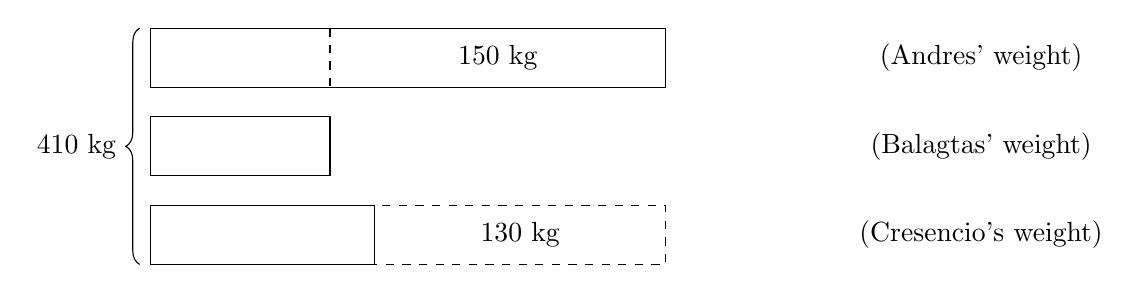
\begin{tikzpicture}[yscale=0.75,xscale=0.01mm]
\draw (0,3) rectangle +(80,1);
\draw (80,3) rectangle +(150,1);
\draw [white] (80,4) -- ++(0,-1);
\draw [dashed] (80,4) -- ++(0,-1);
\node at ($(80,3)!0.5!(230,4)$) {150 kg};
\draw (0,1.5) rectangle +(80,1);
\draw (0,0) rectangle +(100,1);
\draw [dashed] (100,0) rectangle (230,1);
\node at ($(100,0)!0.5!(230,1)$) {130 kg};
\draw [decoration={brace,amplitude=5pt},decorate] (-5,0) -- (-5,4) node [left,pos=0.5,xshift=-5pt,align=center] {410 kg};
\node [xshift=300] at (0,3.5) {(Andres' weight)};
\node [xshift=300] at (0,2) {(Balagtas' weight)};
\node [xshift=300] at (0,0.5) {(Cresencio's weight)};
\end{tikzpicture}

We can see from the diagram that the difference between Andres' and Balagtas' weights is 150 kg,
and the difference between Andres' and Cresencio's weights is 20 kg. Notice that this 20 kg
difference is the additional weight of Cresencio compared to Balagtas' weight. Thus, if we subtract
150 kg and 20 kg from their total weight, this would give us the weight of the three(assuming their
weights are the same) $410 - 150 - 20 = 240$. Now if their weights are the same, this implies that
each of them weigh 80 kg. But since Andres weighs 150 kg more than Balagtas, therefore he weighs
$150 + 80 = 230$ kg.

\Item Mrs. Evangelista bought some mangoes and bananas. The ratio of the number of mangoes
to the number of bananas that she bought was $2:5$. She gave 3/4 of the mangoes to her niece Amparo
and 34 bananas to her nephew Jose. The ratio of the mangoes to bananas is now $2:3$. How many
mangoes and bananas did Mrs. Evangelista buy?

Easily, we can represent the number of mangoes to the number of bananas as follows:

\begin{tikzpicture}[yscale=0.75,xscale=1.5]
\foreach \x in {0,1}
	\draw (\x,0) rectangle +(1,1);
\foreach \x in {0,1,2,3,4}
	\draw (\x,-1.5) rectangle +(1,1);
\node at (7,0.5) {mangoes};
\node at (7,-1) {bananas};
\end{tikzpicture}

Now, she gave 3/4 of the mangoes to her niece and 34 bananas to her nephew. From the diagram, it is
difficult to represent 3/4 of the mangoes. So we will devise a way on how to represent this scenario in
such a way that we are not changing the given in the problem.

\Item Let us make the previous diagram such that we can represent 3/4 of the mangoes more clearly. Let us
draw 3 more sets of the mangoes and 3 more sets of the bananas so as not to change the ratio $2:5$.

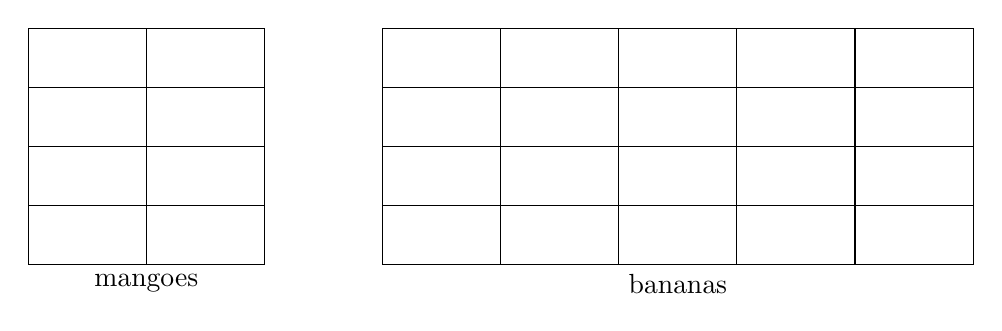
\begin{tikzpicture}[xscale=1.5,yscale=0.75]
\foreach \x in {0,1}
	\foreach \y in {0,1,2,3}
		\draw (\x,\y) rectangle +(1,1);
\node at (1,0) [below] {mangoes};
\begin{scope}[xshift=3cm]
\foreach \x in {0,1,2,3,4}
	\foreach \y in {0,1,2,3}
		\draw (\x,\y) rectangle +(1,1);
\node at (2.5,0) [below] {bananas};
\end{scope}
\end{tikzpicture}

Now from this diagram, we can take away 3/4 of the mangoes.

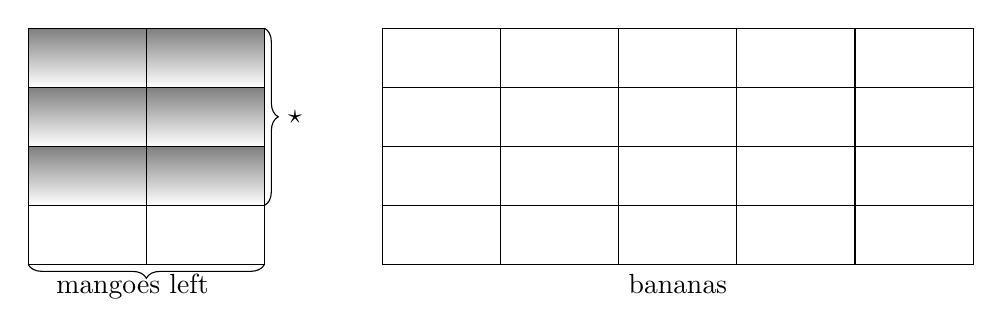
\begin{tikzpicture}[xscale=1.5,yscale=0.75]
\foreach \x in {0,1}
	\draw (\x,0) rectangle +(1,1);
\foreach \x in {0,1}
	\foreach \y in {1,2,3}
		\shadedraw [black,draw=black] (\x,\y) rectangle +(1,1);
\draw [decoration={brace,amplitude=5pt},decorate] (2,0) -- (0,0) node [below,pos=0.5,xshift=-5pt,align=center] {mangoes left};
\draw [decoration={brace,amplitude=5pt},decorate] (2,4) -- (2,1) node [right,xshift=5pt,pos=0.5,align=center] {$\fontsize{24}{24}\star\selectfont$};
\begin{scope}[xshift=3cm]
\foreach \x in {0,1,2,3,4}
	\foreach \y in {0,1,2,3}
		\draw (\x,\y) rectangle +(1,1);
\node at (2.5,0) [below] {bananas};
\end{scope}
\end{tikzpicture}

$\star$ mangoes given to her niece

Now how do we represent the 34 bananas given to her nephew? Take note that each of the
individual rectangle does not correspond to 1 banana. But we know that after giving the 34 bananas,
Mrs. Evangelista was left with mangoes and bananas in the ratio 2:3. Therefore, from the 20
rectangles of the bananas we can take away 17 of them so she's left with the ratio 2:3.

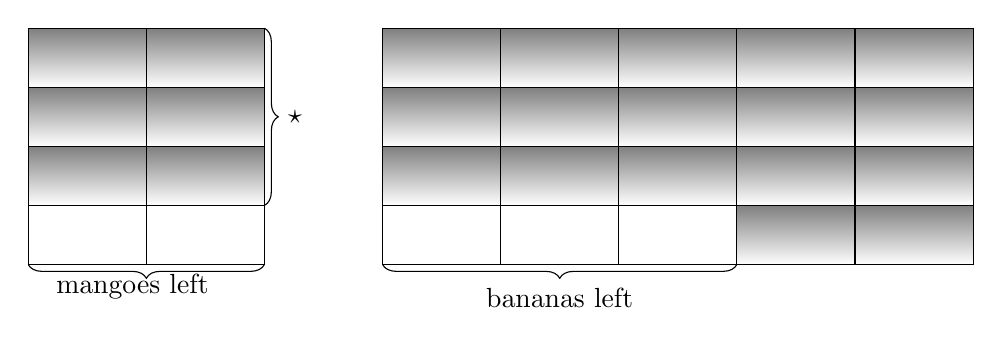
\begin{tikzpicture}[xscale=1.5,yscale=0.75]
\foreach \x in {0,1}
	\draw (\x,0) rectangle +(1,1);
\foreach \x in {0,1}
	\foreach \y in {1,2,3}
		\shadedraw [black,draw=black] (\x,\y) rectangle +(1,1);
\draw [decoration={brace,amplitude=5pt},decorate] (2,0) -- (0,0) node [below,pos=0.5,xshift=-5pt,align=center] {mangoes left};
\draw [decoration={brace,amplitude=5pt},decorate] (2,4) -- (2,1) node [right,xshift=5pt,pos=0.5,align=center] {$\fontsize{24}{24}\star\selectfont$};
\begin{scope}[xshift=3cm]
\foreach \x in {0,1,2}
	\draw (\x,0) rectangle +(1,1);
\foreach \x in {3,4}
	\shadedraw (\x,0) rectangle +(1,1);
\foreach \x in {0,1,2,3,4}
	\foreach \y in {1,2,3}
		\shadedraw [black,draw=black] (\x,\y) rectangle +(1,1);
\draw [decoration={brace,amplitude=5pt},decorate] (3,0) -- (0,0) node [below,pos=0.5,yshift=-5pt,align=center] {bananas left};
\end{scope}
\end{tikzpicture}

The 17 rectangles are equal to the 34 bananas given to his nephew, which means that each rectangle
represents 2 bananas. And each of the rectangles on the left represents 2 mangoes. From this, we
can conclude that originally, Mrs. Evangelista bought $16 (8 \times 2)$ mangoes and $40 (20 \times 2)$ bananas.

\Item Adia and Elijah had the same amount of money at first. When Adia gave Php 18 to Elijah,
Elijah then had five times as much money as his sister. How much money do Adia and Elijah have
together?

\Solution

Before Adia gave Php 18 to Elijah, They both have the same amount of money, which we can represent as follows:

\begin{tabular}[t]{m{1cm}l}
Adia: & \tikz [xscale=1.5,yscale=0.75] \draw (0,0) rectangle (3,1);\\
Elijah & \tikz [xscale=1.5,yscale=0.75] \draw (0,0) rectangle (3,1);\\
\end{tabular}

But after receiving Php 18 from his sister, Elijah had five times as much money as Adia.

\begin{tabular}[t]{m{1cm}l}
Adia: & \tikz [xscale=1.5,yscale=0.75] \draw (0,0) rectangle (1,1);\\
Elijah & \tikz [xscale=1.5,yscale=0.75] \foreach \x in {0,1,2,3,4} \draw (\x,0) rectangle +(1,1);\\
\end{tabular}

Notice that if we move the two blocks from Elijah's to Adia's, they will have the same number of
blocks. This implies that the two blocks are equivalent to the Php 18 that Adia gave to Elijah.
Therefore,
\begin{align*}
\tikz [baseline={([yshift=-3pt]current bounding box.center)},xscale=1.5,yscale=0.75] \foreach \x in {0,1} \draw (\x,0) rectangle +(1,1); &= \Php 18\\
\text{So}\quad \tikz [baseline={([yshift=-3pt]current bounding box.center)},xscale=1.5,yscale=0.75] \draw (0,0) rectangle (1,1); &= \Php 9
\end{align*}
Since they have a total of 6 blocks, $then 6(9) = 54$. Hence, Adia and Elijah have \Php{} 54 altogether.

Andres weigh 150 kg more than Balagtas. Cresencio weigh 130 kg less than Andres. Altogether the
three weigh 410 kg. What is the weight of Andres?
\end{example}

\section*{EXERCISES}
Answer the following problems using the block model.
\begin{enumerate}
\item One number is greater than half of another number by 15. What are the two numbers if
their sum is 48?
\item Mrs. Cruz is using the following recipe in making a juice cocktail: 1/2 cup of pineapple juice $+$ 3/4
cup of mango juice $+$ 1 1/4 cup of apple juice. She will be hosting a party this coming
Saturday. How much of each type of juice will she need if she wants to make 5 liters of this
juice cocktail?
\item A sum of money was divided among Elena, Felicisima, and Gracia in the ratio 2:4:5. Had the
sum of money been equally divided among them, Elena's share would have been larger by
Php 3000. What was the total sum of money?
\item Ben and Caloy are coin collectors. Initially 1/5 of Caloy's coins were equal to 1/3 of Ben's
coins. If Ben gave 24 coins to Caloy, Caloy would have thrice as many coins as Ben. How
many coins did each of them have originally?
\end{enumerate}

\section*{SUGGESTED ACTIVITY}
The participants are tasked to create/design your own word problems (3 word problems
each) using the block model. The level of difficulty of the problems should be easy, average and
difficult. Make sure to have your solution for each of the problem. Write your word problems and
the corresponding solutions to the papers provided for you. You are given 1 1/2 hours to accomplish
the task. After which, some of you will be asked to present his/her output to the rest of the
participants.

\printbibliography[keyword=Module7,heading=subbibliography,title={REFERENCES}]
\chapter{GEOMETRY:\\ INQUIRY-BASED APPROACH}
\section*{INTRODUCTION}
This module presents Inquiry-Based Learning (IBL) as an alternative teaching strategy in
introducing geometry. The first part of the model will let the participants experience an inquiry-
based activity. After which, the activity will be examined on how it was implemented. From the
discussion, definition as well as some models of inquiry-based learning will be discussed. In the
afternoon, participants will have to develop their own lesson plan, activity or worksheet using
inquiry-based learning. Outputs will then be presented for comments and critiquing. Aside from
the models, sample activities, lesson plans, and assessment will also be included.
\section*{OBJECTIVES}
After completing this module, you should be able to:
\begin{enumerate}
\item Experience inquiry-based lesson.
\item Define Inquiry-Based Learning including its factors and essential elements.
\item Identify different models for Inquiry-Based Learning.
\item Develop inquiry-based activity sheets for geometry.
\end{enumerate}
\section*{MATERIALS}
\begin{tabular}{lll}
LCD Projectors & Manila Papers & White Board Markers\\
Permanent Markers & Colored and White Chalks & Bond Markers\\
\end{tabular}

\underline{For Group Activity 1 ( 1 set per group of 5 or 6 participants)}

\begin{tabular}{llll}
Manipulatives & Pencils & Ruler/Meter Stick & Permanent Marker\\
Manila Paper & Crayons & Masking tape & \\
\end{tabular}

\underline{For Group Activity 2 ( 1 set per group of 5 or 6 participants)}

\begin{tabular}{lll}
Manila Paper & Permanent Marker & Masking Tape \\
\end{tabular}

\section*{GROUP ACTIVITY 1}
Participants are to be divided into groups of 5 or 6. This can be done through ice
breakers such as “The Boat is Sinking...” or other games (You may also refer to the site
\url{http://www.girlscoutsnorcal.org/documents/LE-Fun_Splitters.pdf}).

After the groups have settled down and formed a circle, each group will be given an
envelope containing the set of manipulatives with the instructions and guide questions. One set
of manipulatives contains the following figures: square, rectangle, rhombus, parallelogram,
trapezoid, isosceles trapezoid, and kite. Figures may be of different sizes. Answers and outputs
will be written/drawn on a manila paper.

\subsection*{PROCEDURE}

\begin{enumerate}
\item Open the envelope and place the contents on the table/floor.
Guide Questions:
	\begin{enumerate}
	\item Are you familiar with these shapes/figures?
	\item Do you know the names of these figures?
	\end{enumerate}
\item Classify the given figures. Guide Questions:
	\begin{enumerate}
	\item How would you classify these figures?
	\item How many classifications can you make?
	\end{enumerate}
\item Write a general description for each type of classification that you made, as well as
specific descriptions for the figures.
\item Match the following words with the descriptions that you wrote:

\begin{tabular}{llll}
Quadrilateral & Parallelogram & Kite & Trapezoid\\
Rectangle & Rhombus & Square & Isosceles Trapezoid\\
\end{tabular}
\item Draw a concept diagram showing the classification of the figures and how each group of
figures is related to one another.

Guide questions:
\begin{enumerate}
\item How are these figures related to one another?
\item Does your concept map clearly show the hierarchy of the different figures?
\end{enumerate}
\item Based on your concept diagram, determine if the following statement is \textbf{Always},
\textbf{Sometimes}, or \textbf{Never True}.
\begin{enumerate}
\item A kite is a parallelogram.
\item A rhombus is a square.
\item A square is a rhombus.
\item Squares are rectangles.
\item Rectangles are squares.
\end{enumerate}
\end{enumerate}
\begin{definition}[Quadrilaterals]
Let $A$, $B$, $C$, and $D$ be four points in the same plane. If no three of these points are
collinear, and the segments $AB$, $BC$, $CD$, and $DA$ intersect only at their endpoints, then the union
of these four segments is called a \Bold{quadrilateral}. A \Bold{parallelogram} is a quadrilateral in which both pairs of opposite sides are parallel. A \Bold{trapezoid} is a quadrilateral in which one and only one pair of opposite sides is parallel. An \Bold{isosceles trapezoid} is a trapezoid whose non-parallel sides are congruent. A \Bold{rhombus} is a parallelogram whose sides are all congruent. A \Bold{rectangle} is a parallelogram whose angles are all right angles. A \Bold{square} is a rectangle whose sides are all congruent. A \Bold{kite} is a quadrilateral with two pairs of congruent adjacent sides.
\end{definition}
Examples of quadrilaterals are show in Figure \eqref{chap8fig:1}.
\begin{figure}[!h]
\centering
\subfigure[chap8fig:2][A \Bold{convex} quadrilateral.]{
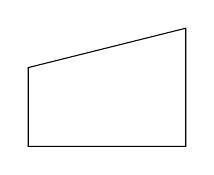
\begin{tikzpicture}
\draw (0,0) -- (2,0) -- (2,1.5) -- (0,1) -- cycle;
\end{tikzpicture}
}\quad
\subfigure[chap8fig:3][A \Bold{concave} quadrilateral.]{
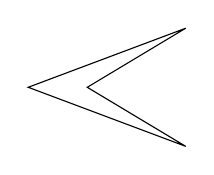
\begin{tikzpicture}[yscale=0.75]
\draw (0,1) -- (2,0) -- (0.75,1) -- (2,2) -- cycle;
\end{tikzpicture}
}\quad
\subfigure[chap8fig:4][A parallelogram.]{
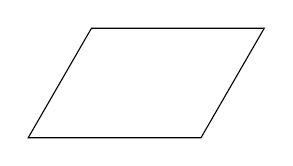
\begin{tikzpicture}
\node [trapezium,trapezium left angle=60, trapezium right angle=120,minimum height=1cm,minimum width=3cm,draw] {};
\end{tikzpicture}
}\\
\subfigure[chap8fig:5][A trapezoid.]{
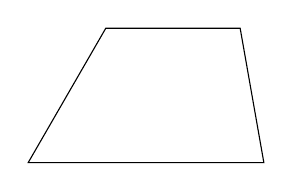
\begin{tikzpicture}
\node [trapezium,trapezium left angle=60, trapezium right angle=80,minimum height=1cm,minimum width=3cm,draw] {};
\end{tikzpicture}
}\quad
\subfigure[chap8fig:6][An isosceles trapezoid.]{
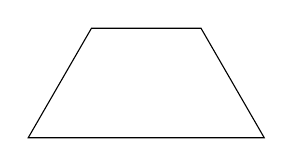
\begin{tikzpicture}
\node [trapezium,minimum height=1cm,minimum width=3cm,draw] {};
\end{tikzpicture}
}\quad
\subfigure[chap8fig:7][A rhombus.]{
\begin{tikzpicture}
\node [trapezium,trapezium left angle=60, trapezium right angle=120,minimum height=1.5cm,minimum width=1.5cm,draw] {};
\end{tikzpicture}
}\\
\subfigure[chap8fig:8][A rectangle.]{
\begin{tikzpicture}
\node [rectangle,minimum height=1.5cm,minimum width=2.5cm,draw] {};
\end{tikzpicture}
}\quad
\subfigure[chap8fig:9][A square.]{
\begin{tikzpicture}
\node [rectangle,minimum height=1.5cm,minimum width=1.5cm,draw] {};
\end{tikzpicture}
}\quad 
\subfigure[chap8fig:10][A kite.]{
\begin{tikzpicture}
\node [kite,kite upper vertex angle=60,kite lower vertex angle=120,minimum width=1.5cm,draw] {};
\end{tikzpicture}
}
\caption{Examples of parallelograms.}
\label{chap8fig:1}
\end{figure}

\begin{figure}[!h]
\centering
\caption{Concept Diagram for Quadrilaterals}
\begin{tikzpicture}
\node (quadrilateral) at (0,0) {};
\draw (quadrilateral)-- +(1.5,0) -- +(1.5,1.175) -- +(0,.67) -- cycle;
\node (B) [below] at ($(quadrilateral)+(1,0)$) {Quadrilateral};
\node (kite) [below left=of B,kite,kite upper vertex angle=120,kite lower vertex angle=60,minimum width=1cm,draw,label=below:kite] {};
\node (parallelogram) [below=of B,trapezium,trapezium left angle=60, trapezium right angle=120,minimum height=0.5cm,minimum width=1.5cm,draw,label=below:parallelogram] {};
\node (trapezoid) [below right=of B,trapezium,trapezium left angle=60, trapezium right angle=80,minimum height=0.5cm,minimum width=1.5cm,draw,label=below:trapezoid] {};
\node (rhombus) [below left=of parallelogram,kite,kite upper vertex angle=60,kite lower vertex angle=60,minimum height=1cm,draw,label=below:rhombus] {};
\node (rectangle) [below right=of parallelogram,rectangle,minimum height=.5cm,minimum width=1.25cm,draw,label=below:rectangle] {};
\node (isosceles trapezoid) [below right=of trapezoid,trapezium,minimum height=.5cm,minimum width=1.5cm,draw,label=below:isosceles trapezoid] {};
\node (square) [below right= of rhombus,rectangle,minimum height=1cm,minimum width=1cm,draw,label=below:square] {};
\begin{pgfonlayer}{background}
\draw ($(quadrilateral)!.5!(0,.67)$) -| (kite);
\draw (1.5,0.33) -| (trapezoid);
\draw (B) -- (parallelogram);
\draw (kite) -- (rhombus);
\draw (parallelogram) -- (rhombus);
\draw (parallelogram) -- (rectangle);
\draw (rhombus) -- (square);
\draw (rectangle) -- (square);
\draw (trapezoid.south) --  (isosceles trapezoid);
\end{pgfonlayer}
\end{tikzpicture}
\label{chap8fig:2}
\end{figure}

Additional Questions:
\begin{enumerate}
\item When can a rectangle be a square?
\item Can a rectangle be a rhombus? How?
\item Can a kite be a rhombus? How?
\end{enumerate}
Answers:
\begin{enumerate}
\item A rectangle can be a square if all the sides of the rectangle are congruent.
\item If a rectangle is a square, then it automatically becomes a rhombus.
\item A kite can become a rhombus if the two pairs of congruent sides are congruent
to one another.
\end{enumerate}
\section*{DISCUSSION}
After Activity 1 has been implemented and discussed, the participants will now examine what
happened during the activity itself. Each step of the activity will be examined for their reaction
or behavior.
\subsection*{Questions for Discussion}
\begin{enumerate}
\item After the envelopes were distributed, what did the members do? How did they behave?
Were they excited, happy, anxious, or indifferent?
\item When you were asked to classify the figures, what was the first thing that came to your
mind? What were the initial questions raised during the discussion?
\item Did everyone participate or contribute in doing the activity? What were the difficulties
encountered by the group? How did you overcome these difficulties?
\item What was the role of the teacher during the entire activity?
\end{enumerate}
In Activity 1, the teacher did not directly lecture on the topic to be discussed but
instead, the participants were given an activity to discover the relationship between the
figures given. Participants were doing more of the learning through the manipulatives and
the guide questions given by the teacher.

This type of activity is an example of an inquiry-based approach of learning.

\subsection*{What is Inquiry-Based Learning?}

As defined by the Brigham Young University’s Center for Teaching and Learning, Inquiry-
Based Learning is

\begin{Quote}
“an inductive teaching methodology that centers around students focusing on
questions and/or research (Spronken-Smith et al., 2008). Teachers engage
students by allowing them to facilitate their own learning with support and
may allow students to create their own learning situations (Spronken-Smith et
al., 2008; Feletti, 1993). “Inquiry learning” was founded around the scientific
method while “inquiry-based learning” was developed as a flexible alternative
to problem-based learning (Feletti, 1993).”
\end{Quote}
Inquiry-based learning is a teaching strategy which involves the learner more than the
traditional way of teaching. In this strategy, learners are guided to understand the concepts.
Dictionary defines inquiry as seeking knowledge, information, or truth through questioning.
Inquiry-based learning is not just asking questions, but it is a way of converting data and
information into useful knowledge. A useful application of inquiry-based learning involves many
different factors, which are, a different level of questions, a focus for questions, a framework for
questions, and a context for questions.

\subsection*{What are the types of questions?}
\begin{definition}[Types of questions in IBL]
\begin{enumerate}
\item \Bold{Inference questions}
	\begin{itemize}
	\item Mainly asked by students who want to gain extra knowledge about a
	particular topic
	\item Students can be encouraged by finding clues, examining them, and
	discussing them to justify the inferences of the topic
	\end{itemize}
\item \Bold{Interpretation questions}
	\begin{itemize}
	\item Mainly force the students to understand the consequences of the ideas
	or information
	\end{itemize}
\item \Bold{Transfer questions}
	\begin{itemize}
	\item Make students take their information to a new place, level or stage
	\end{itemize}
\item \Bold{Hypothesis questions}
	\begin{itemize}
	\item Mainly based on what can be predicted or tested through thinking
	\end{itemize}
\end{enumerate}
\end{definition}
\subsection*{What are the key principles for Inquiry-Based Learning?}
\begin{definition}[Key Principles for IBL]
\begin{enumerate}
\item \textbf{Principle 1:} All learning activities should focus on using information-processing skills (from observations to synthesis) and applying the discipline "ground rules" as a means to learn content set in a
broad conceptual context.
\item \textbf{Principle 2:} Inquiry learning puts the learner at the center of an active learning process, and the systemic
elements (the teacher, instructional resources, technology, and so forth) are prepared or aligned to support the learner.
\item \textbf{Principle 3:} The role of the teacher becomes one of facilitating the learning process. The teacher also becomes a learner by finding out more about the learner and the process of inquiry learning.
\item \textbf{Principle 4:} What is assessed is what is valued. Therefore, more emphasis needs to be placed on assessing the development of information-processing skills, nurtured habits of mind, or "ground rules" of
the discipline, and conceptual understandings rather than just the content of the field.
\end{enumerate}
\end{definition}
Inquiry-Based Learning generally follows the basic inquiry process as shown in Figure \eqref{chap8fig:3}.
There are five key elements in inquiry learning--Ask, Investigate, Create, Discuss and Reflect.
\begin{figure}[!h]
\centering
\smartdiagramset{module shape=ellipse}
\smartdiagram[circular diagram]{Ask, Investigate, Create, Discuss, Reflect}
\caption[Basic Inquiry Process]{The \Bold{Basic Inquiry Process}. Based on: \url{http://www.cii.illinois.edu/InquiryPage/inquiry/process.html}}
\label{chap8fig:3}
\end{figure}
\begin{description}
\item[Ask] It begins with the desire to discover. Meaningful questions are inspired
by genuine curiosity about real-world experiences. A question or a
problem comes into focus at this stage, and the learner begins to define
or describe what it is.

Some real examples of questions in this stage of the process are:
	\begin{itemize}
	\item "What makes a poem poetry?"
	\item "Where do chickens come from and how does an egg 'work'?"
	\item "Why does the moon change shape?"
	\end{itemize}
Of course, questions are redefined throughout the learning process. We
never fully leave one stage and go neatly to the next. As one teacher at a
recent Inquiry Workshop pointed out, "It's messy, but it works!"
Questions naturally lead to the next stage in the process: Investigation.
\item[Investigate] Taking the curious impulse and putting it into action is what we call the
investigation process. At this stage the learner begins to gather
information: researching resources, studying, crafting an experiment,
observing, or interviewing, to name a few. The learner may recast the
question, refine a line of query, or plunge down a new path that the
original question did not or could not anticipate. The information-
gathering stage becomes a self-motivated process that is wholly owned
by the engaged learner.
\item[Create] As the information gathered in the investigation stage begins to
coalesce, the learner begins to make connections. The ability at this
stage to synthesize meaning is the creative spark that forms all new
knowledge. The learner now undertakes the creative task of shaping
significant new thoughts, ideas, and theories outside of his/her prior
experience.
\item[Discuss] At this point in the circle of inquiry, learners share their new ideas with
others. The learner begins to ask others about their own experiences
and investigations. Shared knowledge is a community-building process,
and the meaning of their investigation begins to take on greater
relevance in the context of the learner's society. Comparing notes,
discussing conclusions, and sharing experiences are all examples of this
process in action.
\item[Reflect] Reflection is just that: taking the time to look back at the question, the
research path, and the conclusions made. The learner steps back, takes
inventory, makes observations, and possibly makes new decisions. Has a
solution been found? Do new questions come into light? What might
those questions be?
\end{description}
What follows are other models which are accepted and used in inquiry learning.
\subsection*{Predict--Observe--Explain (POE)}
The POE strategy was developed by White and Gunstone (1992) to uncover individual students'
predictions, and their reasons for making these, about a specific event.
\subsubsection*{When to Use}
POE is a strategy often used in science. It works best with demonstrations that allow immediate
observations, and suits Physical and Material World contexts. A similar strategy also works well in
mathematics, particularly in statistics.
\begin{itemize}
\item It can be used for finding out students' initial ideas;
\item providing teachers with information about students' thinking;
\item generating discussion;
\item motivating students to want to explore the concept; and
\item generating investigations.
\end{itemize}
\subsubsection*{The Theory}
Constructivist theories of learning consider that students’ existing understandings should be
considered when developing teaching and learning programmes. Events that surprise create
conditions where students may be ready to start re-examining their personal theories.
\subsubsection*{How the Strategy Works}
\begin{itemize}
\item Unless students are asked to predict first what will happen, they may not observe
carefully.
\item Writing down their prediction motivates them to want to know the answer.
\item Asking students to explain the reasons for their predictions gives the teacher indications
of their theories. This can be useful for uncovering misconceptions or developing
understandings they have. It can provide information for making decisions about the
subsequent learning.
\item Explaining and evaluating their predictions and listening to others' predictions helps
students to begin evaluating their own learning and constructing new meanings.
\end{itemize}
\subsubsection*{What to Do}
\begin{itemize}
\item Set up a demonstration of an event, related to the focus topic, that may surprise students,
and which can be observed.
\item Tell the students what you are going to be doing.
\end{itemize}
\paragraph*{Step 1: Predict}
\begin{itemize}
\item Ask the students to independently write their prediction of what will happen.
\item Ask them what they think they will see and why they think this.
\end{itemize}
\paragraph*{Step 2: Observe}
\begin{itemize}
\item Carry out the demonstration.
\item Allow time to focus on observation.
\item Ask students to write down what they observe.
\end{itemize}
\paragraph*{Step 3: Explain}
\begin{itemize}
\item Ask students to amend or add to their explanation to take account of the observation.
\item After students have committed their explanations to paper, discuss their ideas together
\end{itemize}
\subsection*{Problem-Based Learning}
At the University of Delaware, they use Problem-based learning in their undergraduate
courses. According to them, in a problem-based learning (PBL) model, students engage complex,
challenging problems and collaboratively work toward their resolution. PBL is about students
connecting disciplinary knowledge to real-world problems--the motivation to solve a problem
becomes the motivation to learn.

With PBL, the teacher gives the students problems to work on and not the lectures or
exercises or assignments. Content is not readily given. Instead, students should work on the
given problem to draw out the necessary concepts to be learned. The teacher acts as a
facilitator who will guide the students in solving the problems instead of being the source of
solutions.

Problem-based learning will provide the students opportunities for the following:
\begin{itemize}
\item examine and try out what they know;
\item discover what they need to learn;
\item develop their people skills for achieving higher performance in teams;
\item improve their communications skills;
\item state and defend positions with evidence and sound argument;
\item become more flexible in processing information and meeting obligations; and
\item practice skills that they will need after their education.
\end{itemize}
An example of how the students can learn through PBL is shown below using a simplified
model for PBL.
\begin{enumerate}
\item \textit{Explore the issues.} 

Your teacher introduces an "ill-structured" problem to you.
Discuss the problem statement and list its significant parts.
You may feel that you don't know enough to solve the problem but that is the
challenge!

You will have to gather information and learn new concepts, principles, or skills as you
engage in the problem-solving process.

\item \textit{List "What do we know?"} What do you know to solve the problem?
This includes both what you actually know and what strengths and capabilities each
team member has.
Consider or note everyone's input, no matter how strange it may appear: it could hold a
possibility!

\item \textit{Develop, and write out, the problem statement in your own words.} 

A problem statement should come from your/the group's analysis of what you know,
and what you will need to know to solve it. You will need:

	\begin{itemize}
	\item a written statement
	\item the agreement of your group on the statement; and
	\item feedback on this statement from your instructor.
	(This may be optional, but is a good idea.)
	
	\textit{Note:} The problem statement is often revisited and edited as new information is
	discovered, or "old" information is discarded.
	\end{itemize}
\item\label{chap8item:1} \textit{List out possible solutions.} List them all, then order them from strongest to weakest.
Choose the best one, or most likely to succeed.
\item \textit{List actions to be taken with a timeline.} 
	\begin{itemize}
	\item What do we have to know and do to solve the problem?
	\item How do we rank these possibilities?
	\item How do these relate to our list of solutions?
	Do we agree?
	\end{itemize}
\item \textit{List "What do we need to know?"}

Research the knowledge and data that will support your solution.
You will need to information to fill in missing gaps.
	\begin{itemize}
	\item Discuss possible resources, such as experts, books, web sites, etc.
	\item Assign and schedule research tasks, and their corresponding deadlines.
	\end{itemize}
If your research supports your solution, and if there is general agreement, go to item \eqref{chap8item:2}.
If not, go back to item \eqref{chap8item:1}.

\item \label{chap8item:2}\textit{Write up your solution with its supporting documentation, and submit it.} You may need to present your findings and/or recommendations to a group or your
classmates. This should include the problem statement, questions, data gathered, analysis of data, and
support for solutions or recommendations based on the data analysis, in short, the process
and outcome.

\item \textit{Present and defend your conclusions.} The goal is to present not only your conclusions, but the foundation upon which they
rest. Prepare to:
	\begin{itemize}
	\item state clearly both the problem and your conclusion;
	\item summarize the process you used, options considered, and difficulties encountered;
	\item convince, not overpower;
	(Bring others to your side, or to consider without prejudice your supporting
	documentation and reason.)
	\item help others learn, as you have learned; and
	\item if challenged and you have an answer, present it clearly.
	(If you don't have an answer, acknowledge it and refer it for more consideration.)
	\end{itemize}
\end{enumerate}
\subsection*{5E Instructional Model}
The 5E's instructional model provides a format for lessons that
builds on what students already know. The 5E's sequence the
learning experience so that learners construct their
understanding of a concept across time. Each phase of the
learning sequence can be described using five words that begin
with "E": Engage, Explore, Explain, Extend, and Evaluate.
\begin{figure}[!h]
\centering
\includegraphics[width=0.3\linewidth]{5E}
\caption[The 5E Instructional Model]{Source: \fullcite{5eim}}
\label{chap8fig:4}
\end{figure}
\begin{longtable}{@{}>{\bfseries\arraybackslash}lp{0.3\linewidth}p{0.3\linewidth}@{}}
\kill
\caption{Sequences of the 5E Instructional Model\label{chap8tab:1}}\\
\hline \hline
\textbf{Learning Phase} & \textbf{Student Rule} & \textbf{Teacher Rule}\\
\hline \hline
\endfirsthead
\caption[]{(continued)}\\
\hline \hline 
\textbf{Learning Phase} & \textbf{Student Rule} & \textbf{Teacher Rule}\\
\hline \hline
\endhead
\hline \hline 
\multicolumn{3}{l}{Continued to next page}\\
\hline
\endfoot
\endlastfoot
Engage/Excite & Students are introduced to the concept. 
Students make connections to prior 
knowledge and what is to be studied. 
Student thinking is clarified. Students 
become mentally engaged in the new 
learning experience. &
Teachers ask questions of
students and engage them in the
guided inquiry lessons. They use
strategies that make connections
between the past and present
learning experience. Teachers set
a level of anticipation.\\
Explore & Students explore or experiment at this point. 
They engage in observations, use science 
tools and materials (manipulatives), collect 
data, and record data. &
Teachers set up the investigation
and guide students in inquiry,
asking probing questions to clarify
understanding.\\
Explain & Students verbalize their understandings from 
the "explore" phase, look for patterns in 
their data, and describe what they observed. 
This can be done in small and/or whole 
groups. & 
Teachers ask probing questions
that encourage students to look
for patterns or irregularities in
their data.\\
Elaborate & Students expand their learning, practice skills 
and behavior, and make connections or 
applications to related concepts and in the 
world around them. & Teachers provide learning
opportunities for students to
apply their knowledge and to gain
a deeper understanding. Activities
can include reading articles and
books, writing, designing other
experiments, and exploring
related topics on the Internet. \\
Evaluate & Students answer questions, pose questions, 
and illustrate their knowledge 
(understandings) and skills (abilities). & 
Teachers diagnose student
understanding through an
ongoing process. Assessment can
be both formative (ongoing and
dynamic) and summative (end-of-
lesson final test or product).\\
\hline
\end{longtable}
\newpage
\subsection*{7E Instructional Model}
The 7E Instructional model is based on the 5E model but expands the engagement
phase to elicit and engage. The elaborate and evaluate phases are expanded to elaborate,
evaluate and extend, as well. The purpose of the 7E model is to emphasize the importance of
recognizing prior knowledge and expanding knowledge gained through conceptual change
(Eisenkraft, 2003). % No Eisenkraft in References.

\begin{figure}[!h]
\centering
\includegraphics[width=\linewidth]{7E}
\caption[The 7E Instructional Model Used in Active Chemistry]{Source: \fullcite{7eim}}
\label{chap8fig:5}
\end{figure}
These instructional elements will help to structure lessons to be Inquiry based.
\begin{longtable}{@{}>{\bfseries\arraybackslash}lp{0.4\linewidth}@{}}
\kill
\caption{Instructional Elements of the 7E Instructional Model\label{chap8tab:2}}\\
\hline \hline
\endfirsthead
\hline \hline 
\endhead
\hline \hline 
\multicolumn{2}{l}{Continued to next page}\\
\hline
\endfoot
\endlastfoot
Elicit & Identify what students know.\\
Engage & Creates interest
students.\\
Explore & Provides activities and experiments for students to
collect and analyse data\\
Explain & Encourage students to explain concepts followed by
formal explanation by teacher.\\
Elaborate & Provide opportunity for students to apply
knowledge and skills learnt in new but similar
situations.\\
Evaluate & Assess understanding and abilities of the students.\\
Extend & Students try to apply new knowledge and skills in
completely unfamiliar situations.\\
\hline
\end{longtable}
\subsection*{4E $\times$ 2 Instructional Model}
The 4E $\times$ 2 Instructional Model
was designed to unite three major
learning constructs (inquiry instruction,
formative assessment, and reflective
practice) that have all been shown to
improve learning. When well integrated
these learning constructs help facilitate
deeper teaching and more powerful
learning experiences. All the lessons
designed and available under the lesson
plan tab use the 4E $\times$ 2 Model.
\begin{figure}[!h]
\centering
\includegraphics[width=0.5\linewidth]{4ex2}
\caption[$4\mathrm{E}\times 2$ Instructional Model]{\Bold{4E $\times 2$ Instructional Model}. Source: \fullcite{marshall}}
\label{chap8fig:6}
\end{figure}
\subsection*{GROUP ACTIVITY 2}
The participants will again be grouped into 5 or 6. The groupings in the morning may be
retained for this activity.

Each group must come up with their own inquiry-based activity or lesson plan. Each group can
choose one topic among the following to work on. Outputs shall be written on the Manila Paper.

\begin{center}
\begin{tabular}{p{0.3\linewidth}p{0.3\linewidth}}
\hline 
Points, Lines and Planes & Subsets of a Line\\
Different Kinds of Angles & Angle Pairs\\
Vertical Angles and Angles formed by Transversals & Classification of Triangles\\
Relationship of Sides and Angles in Triangles & Convex Polygons\\
Quadrilaterals & Exterior and Interior Angles of Convex Polygons\\
Circles & \\
\hline 
\end{tabular}
\end{center}
\subsection*{SAMPLE ACTIVITIES, LESSON PLAN and LESSON PLAN TEMPLATES}
\begin{itemize}
\item Sum of Interior Angles: \fullcite{sia}
\item Geometry and the Real World: \fullcite{abdul}
\item 5E Lesson Plan: The Geometry for Pentominoes: \fullcite{uoh}
\end{itemize}
After the workshop, each group will present their output to the body for critiquing
and suggestions.
\subsection*{How to Evaluate Inquiry-based Instruction}
The Electronic Quality of Inquiry Protocol (EQUIP) instrument is designed to measure
the quantity and quality of inquiry instruction being facilitated in K-12 math and science
classrooms. The instrument does not seek to measure all forms of quality instruction–only those
that are inquiry-based in nature. \textcite{4e2} provides a form which can be used for peer
evaluation and classroom observations.

Included in this file are four rubrics to evaluate instructional, discourse, assessment, and
curriculum factors. For each construct measured, the evaluator will determine if the implementation of the lesson plan is at pre-inquiry (level 1), developing inquiry (level 2),
proficient inquiry (level 3) or exemplary inquiry (level 4). Pre-inquiry level suggests that it is
more teacher-centered rather than student centered while a rating of 4 would indicate more
student participation in acquiring learning.
\printbibliography[keyword=Module8,heading=subbibliography,title={REFERENCES}]
\chapter[SOLVING WORD PROBLEMS]{SOLVING WORD PROBLEMS\\ IN GEOMETRY}
\section*{INTRODUCTION}
This module is intended to give an overview on solving word problems in geometry. It presents
the different steps in problem solving as designed by Polya. It also contains sample word problems for
the participants to solve. Assessment questions are also given.
\section*{OBJECTIVES}
After completion of the module, the participants are expected to:
\begin{enumerate}
\item Apply the different steps in problems solving
\item Determine the appropriate strategy to use in solving a word problem.
\item Use variety of problem solving strategies in solving word problems.
\item Solve the word problems accurately.
\item Appreciate the importance of problem solving in a mathematics curriculum.
\item Gain confidence in doing problem solving
\item Create more interesting word problems.
\item Integrate or connect geometry to origami, the art of paper folding.
\end{enumerate}
\section*{DISCUSSION}
The National Council of Teachers of Mathematics (NCTM) gives the following definitions on the
nature of mathematics: mathematics is a study of patterns and relationships, it is a way of thinking, it is
an art, it is a language and it is a tool. NCTM identified five broad goals required to meet the students’
mathematical needs for the 21st century. They are as follows: students should (1) value mathematics,
(2) reason mathematically, (3) communicate mathematics, (4) solve problems and (5) develop
confidence.

Problem solving is the heart of mathematics. It is a process. It is the means by which an
individual uses previously acquired knowledge, skills and understanding to satisfy the demands of an
unfamiliar situation. Students must be exposed to a variety of problems – problems that vary in context,
in level of difficulty and in methods in solving the problem. But what is really a problem or a word
problem specifically? A word problem is a mathematical proposition that a student has never
experienced solving. What are the purposes of word problems? The following are the different
purposes of word problems: (1) to prepare the students for real life, (2) to develop children’s logical and
abstract thinking and mental discipline, and (3) to motivate students. Hence a word problem should
simulate real life situations, events, and places that students can experience firsthand. In this way the
students will be able to see the importance of mathematics in their life.

George Polya, a mathematician, devised the following \Bold{four-step method} in solving word problems:

\begin{enumerate}
\item \textbf{Read and understand the problem}\index{four-step method!Read and understand the problem}

Read and reread the problem. Ask the following questions: What is the situation all
about? What information is given? What are the different assumptions? What information is
missing? What are you being asked to find or to do? You can make a list in this format

Information given (GIVEN): \makebox[2in]{\hrulefill}

Goals of the problem (REQUIRED): \makebox[2in]{\hrulefill}

\item \textbf{Plan how to solve the problem. Try a strategy}\index{four-step method!Try a strategy}\index{four-step method!Plan how to solve the problem}

In developing a plan to solve the problem ask the following questions: Have you ever
worked a similar problem before? Will you estimate or calculate? What strategy (ies) can you
use? Consider the different strategies in solving problem that you know. The following could be
your shopping list on the different problem solving strategies: draw a diagram, make a table,
write an equation, guess and check (trial and error), look for a pattern, solve a simpler problem,
work backward. Word problems can be solved using different strategies.

\item \textbf{Solve the problem/ Carry out the plan.}\index{four-step method!solve the problem}\index{four-step method!carry out the plan}

As you implement the strategy that you choose, ask the following questions: Did you
calculate correctly? What is the solution? Did you interpret correctly? Did you answer the
question?

\item \textbf{Look back}\index{four-step method!look back}

Most students forget this last part especially if they are solving a problem set or many
problems. The most important question that should be asked here is: “Is the calculated answer
reasonable?”
\end{enumerate}
However there is also a danger in over-using Polya's four steps in problem solving. Students
may think that problem solving is one directional that follows the given steps above as if it's the
prescribed recipe. Emphasize to students that with challenging problems, the actual problem solving
becomes a process whereby the solver keeps a mental "check" of the progress, and corrects himself if
progress is not made. He may go one route, notice it won't work, go backwards a bit, and then, take
another route. In other words, devising plans and carrying them out can occur somewhat
simultaneously, and we can go back and forth. Lastly, not all problems can be solved using the steps
above.

\subsection*{Problems Involving Perimeters}
\begin{example}
\Item The perimeter of a square is 28 cm. Find the length of each side.

\Solution

\textit{Geometry Concept:} A square is a quadrilateral (4-sided polygon) with four congruent sides. Its four
interior angles are all right angles. The formula for the perimeter ($P$) of a square is $P = 4s$ and its area ($A$) is $A = s^2$ where $s$ is the side of the square.

\begin{tikzpicture}
\draw (0,0) -- (1,0) -- (1,1) -- (0,1) -- cycle;
\node [below] at (0.5,0) {$s$};
\node [right] at (1,0.5) {$s$};
\node [above] at (0.5,1) {$s$};
\node [left] at (0,0.5) {$s$};
\end{tikzpicture}
\begin{align*}
P&=4s\\
28&=4s\\
\therefore s&=7
\end{align*}
Therefore, the square has side of length 7 cm.
\end{example}

\begin{example}
\item The length of a rectangular garden is 3 meters more than its width. If the perimeter of the garden is
50 meters, what is the area of the rectangle?

\Solution

\textit{Geometry Concept}

A rectangle is a quadrilateral (4-sided polygon) with two pairs of congruent
and parallel sides. Its four interior angles are all right angles.
The formula for the perimeter ($P$) of a rectangle is $P = 2L + 2W$ where $L$ is
the length and $W$ is the width of the rectangle.

\begin{tikzpicture}[xscale=2]
\draw (0,0) -- (1,0) -- (1,1) -- (0,1) -- cycle;
\node [below] at (0.5,0) {$L$};
\node [right] at (1,0.5) {$W$};
\node [above] at (0.5,1) {$L$};
\node [left] at (0,0.5) {$W$};
\end{tikzpicture}

\textit{Representation}
\begin{align*}
W&=\text{width of the rectangle}\\
L&=W+3
\end{align*}

\textit{Equation:}
\begin{align*}
50 &= 2(W + 3) + 2W && \text{Using the formula for perimeter.}\\
50 &= 2W + 6 + 2W \\
44 &= 4W \\
W &= 11 \\
L &= 11 + 3 = 14 \\
A &= (14)(11) = 154 && \text{Using the formula for area.}
\end{align*}

Therefore, the rectangle has an area of 154 $\cm^2$.
\end{example}

\begin{example}
\Item The longest side of a triangle is twice as long as the shortest side and is also 2 cm longer than the third side. If the perimeter of the triangle is 33 cm, what is the length of each side?

\Solution

\textit{Geometry Concept:}

A triangle is a 3-sided polygon. The formula for the perimeter ($P$) of a triangle is
$P = a + b + c$ where $a$, $b$ and $c$ are the sides of the triangle.

\begin{tikzpicture}
\draw (0,0) -- (2,0) -- (0.5,1.5) -- cycle;
\node [below] at (1,0) {$c$};
\node [right] at (1.25,0.75) {$b$};
\node [left] at (0.25,0.75) {$a$};
\end{tikzpicture}

\textit{Representation}

\begin{align*}
a&=x && \text{shortest side of the triangle}\\
b&=2x && \text{longest side}\\
c&=2x-2 && \text{third side}
\end{align*}

\textit{Equation}

\begin{align*}
33 &= x + 2x + 2x - 2 && \text{(Using the formula for the perimeter.)}\\
35 &= 5x\\
x &=7\\
a&=x=7\\
b&= 2x = 14\\
c &= 2x - 2 = 12
\end{align*}
Therefore, the sides of the triangle are 7 cm, 12 cm and 14 cm.
\end{example}

\begin{example}
\Item What is the measure of the base of an isosceles triangle if its perimeter is 50 cm and the length of one of its congruent sides exceeds the length of the base by 10 cm?

\begin{tikzpicture}[yscale=2]
\draw (0,0) -- (1,0) -- (0.5,1) -- cycle;
\node [below] at (0.5,0) {base};
\node [right] at (0.75,0.5) {leg};
\node [left] at (0.25,0.5) {leg};
\end{tikzpicture}

\Solution

\textit{Geometry Concept}

An isosceles triangle is a triangle with two congruent sides. The congruent sides are
called legs while the non-congruent side is called the base.

\textit{Representation}

\begin{align*}
x&=\text{length of the base of the triangle}\\
  x+10&=\text{length of the leg of the triangle}
\end{align*}

\textit{Equation}

\begin{align*}
50 &= x + 2(x + 10) && \text{(Using the formula for perimeter of triangles.)}\\
50 &= x + 2x + 20\\
30 &= 3x\\
x &= 10
\end{align*}
Therefore, the base of the isosceles triangle is 10 cm.
\end{example}

\subsection*{PROBLEMS INVOLVING ANGLES OF POLYGONS}
\begin{example}
\Item The first angle of a triangle is triple that of the smallest angle. The second angle is 5 degrees more than the first angle. What is the measure of the smallest angle?

\Solution

\textit{Geometry Concept}

A triangle has three interior angles and their measures sum up to 180 degrees.

\textit{Representation}
\begin{align*}
x &= \text{smallest angle of the triangle}\\
3x &= \text{first angle of the triangle}\\
3x + 5 &= \text{second angle of the triangle}
\end{align*}
\textit{Equation}
\begin{align*}
x + 3x + 3x + 5 &= 180 && \text{(Sum of the angles of a triangle is $180^{\circ}$.)}\\
7x &= 175\\
x &= 25
\end{align*}
Therefore, the measure of the smallest angle of the triangle is 25 degrees.
\end{example}

\begin{example}
\Item One of the base angles of an isosceles triangle measures 15 degrees less than its vertex angle. Find the
measure of its vertex angle.

\textit{Geometry Concept}

In an isosceles triangle, it has two congruent angles opposite the congruent sides. The angle opposite
the base is called the vertex angle.

\Solution

\textit{Representation}

\begin{align*}
x&=\text{vertex angle}\\
x-15 &= \text{base angle}
\end{align*}

\textit{Equation}

\begin{align*}
2(x - 15) + x &= 180 && \text{(Sum of the angles of a triangle is $180^{\circ}$.)}\\
2x - 30 + x &= 180\\
3x &= 210\\
x &= 70
\end{align*}
Therefore, the measure of the vertex angle of the triangle is 70 degrees.
\end{example}

\begin{example}
\Item Given the parallelogram on the right, find the value of $x$.

\begin{tikzpicture}
\node (trap1) [trapezium,trapezium left angle=81,trapezium right angle=99,minimum width=3cm, minimum height=1.5cm,draw] {};
\node [below right] at (trap1.north west) {$(6x-15)^{\circ}$};
\node [above right] at ([xshift=-10pt]trap1.south west) {$(4x+5)^{\circ}$};
\end{tikzpicture}

\textit{Geometry Concept}

A parallelogram is a quadrilateral with two pairs of congruent and parallel sides. Its two pairs of opposite
angles are congruent and the sum of the measures of any two consecutive angles is 180 degrees.

\Solution

\begin{align*}
(4x + 5) + (6x - 15) &= 180 && \text{(The given angles are consecutive.)}\\
10x - 10 &= 180\\
10x &= 190\\
x &= 19
\end{align*}
\end{example}

\begin{example}
\Item Given the rhombus, find the measure of the angles of the rhombus.

\begin{tikzpicture}
\node (trap1) [trapezium,trapezium left angle=45,trapezium right angle=135,minimum width=3cm, minimum height=1.5cm,draw] {};
\node [below right] at ([xshift=-15pt]trap1.north east) {$(6x-15)^{\circ}$};
\node [above left] at ([xshift=15pt]trap1.south west) {$(4x+5)^{\circ}$};
\end{tikzpicture}

\Solution

\textit{Geometry Concept}

A rhombus is a parallelogram with four congruent sides. Just like a parallelogram, its two pairs of
opposite angles are congruent and the sum of the measures of any two consecutive angles is 180
degrees.
%
\begin{align*}
6x - 15 &= 4x + 5 && \text{(The given angles are opposite.)}\\
2x &= 20\\
x &= 10\\
4x + 5 &= 45
\end{align*}
The given opposite angles have a measure of 45 degrees each while its other two angles
measure $180 - 45 = 135$ degrees each.

Therefore, the measures of the angles of the rhombus are $45\degree$, $45\degree$, $135\degree$, and $135\degree$.
\end{example}
\subsection*{PROBLEMS INVOLVING COMPLEMENTARY, SUPPLEMENTARY\\ AND CONGRUENT ANGLES}
\begin{example}
\item Given two intersecting lines, find the value of $x$.

\begin{tikzpicture}[scale=2,thick,>=stealth']
\draw [->] (0,0) -- (22.5:1cm);
\draw [->] (0,0) -- (22.5:-1cm);
\draw [->] (0,0) -- (-22.5:1cm);
\draw [->] (0,0) -- (-22.5:-1cm);
\node [right] at ([xshift=5pt]0,0) {$(6x-15)\degree$};
\node [left] at ([xshift=-5pt]0,0) {$(4x+5)\degree$};
\end{tikzpicture}

\Solution

\textit{Geometry Concept}

The two intersecting lines formed angles and the two given angles are “opposite” each other. They are
called \Bold{vertical angles}. Vertical angles are congruent. 

Since the given angles are vertical angle, they are congruent. Refer to Example 8.

Therefore, the value of $x$ is 10.
\end{example}

\begin{example}
\Item Given two intersecting lines, find the value of $x$.

\begin{tikzpicture}[scale=2,thick,>=stealth']
\draw [->] (0,0) -- (22.5:1cm);
\draw [->] (0,0) -- (22.5:-1cm);
\draw [->] (0,0) -- (-22.5:1cm);
\draw [->] (0,0) -- (-22.5:-1cm);
\node [right] at ([xshift=5pt]0,0) {$(6x-15)\degree$};
\node [below] at ([yshift=-3pt]0,0) {$(4x+5)\degree$};
\end{tikzpicture}

\Solution

\textit{Geometry Concept}

The two intersecting lines formed angles and note that when the measures of the two given angles are
added, we get the measure of a straight angle. These two angles are called linear pairs. The degree
measures of a \Bold{linear pair} sum up to 180 degrees.

Since the given angles are linear pairs, they sum up to $180\degree$. Refer to Example 7. %Fix reference here.

Therefore, the value of $x$ is 19.
\end{example}

\begin{example}
\Item The supplement of an angle is 20 degrees more than thrice the measure of the angle. What is the
measure of the angle?

\Solution

\textit{Geometry Concept:} When the measures of two angles sum up to 180 degrees, they are called \Bold{supplementary angles}.
\begin{align*}
x &= \text{the given angle}\\
180 - x &= \text{the measure of the supplement of the angle}\\
180 - x &= 3x + 20\\
160 &= 4x\\
x &= 40
\end{align*}
Therefore, the measure of the angle is 40 degrees.
\end{example}

\begin{example}
\Item The supplement of a certain angle is four times its complement. What is the measure of the angle?

\Solution

\textit{Geometry Concept:} When the measures of two angles sum up to 90 degrees, they are called \Bold{complementary angles}.
\begin{align*}
x &= \text{the given angle}\\
180 - x &= \text{the measure of the supplement of the angle}\\
90 - x &= \text{the measure of the complement of the angle}\\
180 - x &= 4(90 - x)\\
180 - x &= 360 - 4x\\
3x &= 180\\
x &= 60
\end{align*}
Therefore, the measure of the angle is 60 degrees.
\end{example}
\section*{EXERCISES}
\begin{enumerate}
\item If the width of a rectangle is 2 cm more than one-half its length and its perimeter is 40 cm, what are
the dimensions of the rectangle?
\item Each side of a triangle with sides 3 cm, 4 cm and 5 cm is extended the same amount. If the new
perimeter of the triangle is twice its original perimeter, what is the length of each side of the new
triangle?
\item In a triangle, the ratio of the measures of its sides is 2:3:4 and the perimeter is 72 cm. Find the
measures of the sides of the triangle.
\item In a triangle, the ratio of the measures of its angles is 2:3:4. Find the measures of the angles of the
triangle.
\item If the numerical value of the area of a rectangle is twice the numerical value of its perimeter, and
the length of one of its sides is 4.5, what are the lengths of its the other three sides?
\item The measure of an angle is thrice the measure of its supplement. Find the measure of the
supplement of the angle.
\item What is the measure of an angle if the measure of its supplement is 10 degrees more than twice its
complement?
\item The sum of the measures of an acute angle and an obtuse angle is 1400. The sum of twice the
supplement of the obtuse angle and three times the complement of the acute angle is 3400. Find the
measures of the angles.
\item When a beam of light is reflected from a
smooth surface, the angle formed by the
incoming beam with the surface is congruent
to the angle formed by the reflected beam
and the surface.
Given the following
information, the measure of $\angle ABC$ is 90, the
measure of $\angle BCD$ is 75, and the beam of
light makes an angle of $35\degree$ with line segment
$AR$. At what angle does the beam reflect
from line segment $AB$ the second time. You
can indicate computed measures on the
figure.

$m\angle EAF = \makebox[1.5in]{\hrulefill}$

\item The Leaning Tower of Pisa in Italy makes an angle with the ground of
about $84\degree$ on one side the figure and is denoted by $\degree$. Find the measure of
the other angle that the tower makes with the ground.
\end{enumerate}
\section*{ADDITIONAL PROBLEMS}
\begin{enumerate}
\item The design of the patio of Mr. Archangel is shown at the right. If the measure of $\angle1$ is three times as large as the measure of $\angle 2$, calculate the measure of $\angle 1$.
\begin{center}
\begin{tikzpicture}[scale=0.6]
\node (A) [thick,trapezium,trapezium left angle=90,trapezium right angle =45,rotate=90,draw,minimum width=1cm,minimum height=2cm] {};
\draw ([yshift=1pt,xshift=-0.5pt]A.south west) rectangle ++(-10pt,10pt);
\draw ([yshift=1pt]A.north west) rectangle ++(10pt,10pt);
\node at ([xshift=-10pt,yshift=2.2cm]A.south east) {2};
\node at ([xshift=10pt,yshift=-10pt]A.north east) {1};
\end{tikzpicture}
\end{center}
\Solution

We have here a convex quadrilateral. The some of the measures of
the interior angles of a quadrilateral is 360. Two angles are already
right angles, hence, the sum of their measures is 180. The sum of the
measures of $\angle 1$ and $\angle 2$ is 180.

Setting up an equation, we have the following solution:
Let $x$ be the measure of $\angle 2$. The measure of $\angle 1$ is $3x$ and $x+3x=180$
will be our working equation. Simplifying we have $4x=180$ and simplifying further $x = 45$. Therefore the measure of $\angle 1$ is 135.

\item At night time, it is usually warmer during summer at the urban regions that at the rural regions. Part
of the reasons to this is the amount of heat absorbed by the establishments during the day which
they will emit at night time. The narrow city streets and tall building trap and absorbs the sun's heat
during the day. When sunlight shines on flat land, some of the light scatters back into the sky. In
the city, light scattered by the ground or building often hits another building. Instead of escaping
into the atmosphere the heat is absorbed. The more heat is absorbed the greater is the heat
released at night time. The reflection of light is governed by the law of reflection which states that
the angle of incidence is equal to the angle of reflection. The angle of incidence is the angle formed
by the incident ray and the line perpendicular to the surface called the normal line. On the other
hand, the angle of reflection is the angle formed by the reflected ray and the normal line. The figure
below shows two parallel buildings on the opposite sides of the road. $\ray{AB}$ is the incident line and is reflected along the vertical side of the building. It is reflected as $\ray{BC}$, then reflected again as $\ray{CD}$ and finally as $\ray{DE}$. If the measure of $\angle ABG$ is 35, what is the measure of $\angle FDE$?
\begin{center}
\begin{tikzpicture}[>=stealth']
\newcommand{\Value}{\pgfmathparse{atan(2)}\pgfmathresult}
\node (A1) [pattern=bricks,minimum width=0.5cm,minimum height=3cm,draw] {};
\node (A2) at ([xshift=-0.775cm,yshift=-0.5cm]A1.east) [pattern=bricks,minimum width=0.5cm,minimum height=2cm,draw] {};
\node (A3) at ([xshift=-1.275cm,yshift=-1cm]A1.east) [pattern=bricks,minimum width=0.5cm,minimum height=1cm,draw] {};
\begin{scope}[xshift=3cm]
\node (B1) [pattern=bricks,minimum width=0.5cm,minimum height=3cm,draw] {};
\node (B2) at ([xshift=0.25cm,yshift=-0.5cm]B1.east) [pattern=bricks,minimum width=0.5cm,minimum height=2cm,draw] {};
\node (B3) at ([xshift=0.75cm,yshift=-1cm]B1.east) [pattern=bricks,minimum width=0.5cm,minimum height=1cm,draw] {};
\end{scope}
\coordinate (B) at ([yshift=-10pt]B1.north west) {};
\coordinate (C) at ([xshift=20pt]A1.south east) {};
\draw [->] (B) -- (C);
\coordinate (D) at ([yshift=10pt]A1.south east);
\draw [->] (C) -- (D);
\coordinate (E) at ([yshift=30pt]B1.north west);
\draw [shorten >=-20pt,->] (D) -- (E) node [below right] {$E$};
\draw [->] (D) -- +(0,4cm) node [above] {$F$};
\draw (A1.south east) -- (B1.south west);
\draw [->] (B1.south west) -- +(0,4.5cm) node [above] {$G$};
\coordinate (A) at ($(B)!-2cm!96.57:(C)$);
\draw [->] (A) -- (B);
\node [left] at (A) {$A$};
\node [left] at ([xshift=-2pt,yshift=-2pt]B) {$B$};
\node [below] at (C) {$C$};
\node [right] at ([yshift=3pt]D) {$D$};
\useasboundingbox{(0,3cm)};
\end{tikzpicture}
\end{center}
\Solution

We know that the measure of $\angle ABG$ is 35. We are tasked to find the measure of $\angle FDE$. We
also know that the angle of incidence is equal to the angle of reflection. To solve the problem, we
need to redraw the figure and in each reflection process we draw the normal line. We will also use
the theorem complements of congruent angles are congruent. (The normal line is perpendicular to
the surface. The angle of incidence and the angle formed by the incident ray and the surface are
complementary). For the purpose of clearer solution, we will enlarge the figure and remove the
buildings. The broken arrows are the normal line.
\begin{center}
\begin{tikzpicture}[>=stealth']
\newcommand{\Value}{\pgfmathparse{atan(2)}\pgfmathresult}
\node (A1) [minimum width=0.5cm,minimum height=3cm] {};
\begin{scope}[xshift=3cm]
\node (B1) [minimum width=0.5cm,minimum height=3cm] {};
\end{scope}
\coordinate (B) at ([yshift=-10pt]B1.north west) {};
\coordinate (C) at ([xshift=20pt]A1.south east) {};
\draw [->] (B) -- (C);
\coordinate (D) at ([yshift=10pt]A1.south east);
\draw [->] (C) -- (D);
\coordinate (E) at ([yshift=30pt]B1.north west);
\draw [shorten >=-20pt,->] (D) -- (E) node [below right] {$E$};
\draw [->] (D) -- +(0,4cm) node [above] {$F$};
\draw (A1.south east) -- (B1.south west);
\draw [->] (B1.south west) -- +(0,4.5cm) node [above] {$G$};
\coordinate (A) at ($(B)!-2cm!96.57:(C)$);
\draw [->] (A) -- (B);
\node [left] at (A) {$A$};
\node [right] at ([xshift=-2pt,yshift=-2pt]B) {$B$};
\node [below] at (C) {$C$};
\node [right] at ([yshift=3pt]D) {$D$};
\draw [dashed,->] (D) -- +(2cm,0) node [right] {$J$};
\draw [dashed,->] (C) -- +(0,2cm) node [above] {$I$};
\draw [dashed,->] (B) -- +(-2cm,0) node [left] {$H$};
\node at ([xshift=-5pt]B1.south east) {$K$};
\draw ([xshift=-15pt]B1.south east) rectangle +(-5pt,5pt);
\useasboundingbox{(0,3cm)};
\end{tikzpicture}
\end{center}
The measure of $\angle ABG$ is 35. Therefore its complement ($\angle ABH$) has a measure of 55.
Complementary angles are pair of angles whose some of their measures is equal to 90. $\angle ABH$ is the angle of
incidence while $\angle HBC$ is the angle of reflection. By the
law of reflection these angles ($\angle ABH$ and $\angle HBC$) have equal measure. The normal ray ($\ray{BH}$) is parallel to the surface of the road (since the road and the side of the
building are perpendicular and the normal line is
perpendicular to the side of the building. Lines
perpendicular to the same line are parallel). $\Segment{CB}$ is the transversal and $\angle HBC$ and $\angle BCK$ are alternate interior angles. (Alternate interior angles of parallel lines cut by
a transversal are congruent). Therefore the measure of
$\angle BCK$ is 55. The measure of $\angle BCI$ (angle of incidence)
is 35 since $\angle BCK$ and $\angle BCI$ are complementary.

Using the same processes, the measure of $\angle BCI$ is 35, the measure of $\angle ICD$ is 35, $\angle CDJ$ is 55, $\angle JDE$ is also 55 and finally the measure of $\angle FDE$ is 35.

\item Kaitlin and Henry are participating in a treasure hunt. They are on the same straight path,
walking toward each other. When Kaitlin reaches the Big Oak, she will turn $115\degree$ onto another
path that leads to the treasure. At what angle will Henry turn when he reaches the Big Oak to
continue on to the treasure?

\begin{center}
\begin{tikzpicture}[>=stealth']
\node (cloud) [cloud,minimum width=2cm,minimum height=1cm,cloud ignores aspect,draw] {Big Oak};
\draw [->] (cloud) -- +(0.4\linewidth,0) node [right] (B) {};
\draw [->] (cloud) -- +(-0.4\linewidth,0) node [left] (C) {};
\node (D) at ($(cloud)!0.3\linewidth!-115:(C)$) [cloud,minimum width=2cm,minimum height=1cm,cloud ignores aspect,draw] {Treasure};
\draw (cloud) -- (D);
\node [above] at (B) {
\includegraphics[width=0.5in]{henry}
};
\node [above] at (C) {
\includegraphics[width=0.25in]{kaitlin}
};
\end{tikzpicture}
\end{center}

\Solution

To solve the problem, we need to draw a diagram that illustrates the problem. Below is
the diagram that illustrates the problem. We need to assume that Big Oak, Kaitlin and Henry are
on the same line. The angle formed by the rays joining Kaitlin, Big Oak and treasure has a
measure equal to $115\degree$. Therefore we need to get the measure of the supplement of that angle
since it's the angle where Henry will turn if he will reach Big Oak. Hence, Henry should turn at
$65\degree$-angle to continue to the treasure.
\end{enumerate}
\section*{SUGGESTED ACTIVITY}\pdfmargincomment[author={Joseph S. Tabadero, Jr.},]{Was this copied verbatim from the source? If so, then this has to be paraphrased/re-written.}
This is adopted from Sourcebook on Practical Work for Teacher Trainers: High School Mathematics I and
II Volume 2.
\subsection*{Exploring the Geometry in a Paper Cup}
\subsubsection*{Objectives}
\begin{enumerate}
\item To apply geometric concepts and principles
\item To justify or prove geometric relationships
\end{enumerate}
\subsubsection*{Materials}
\begin{enumerate}
\item 5 pieces of coupon bond
\item 2 square papers
\end{enumerate}
\subsubsection*{Instructional Procedures}
\textit{Introductory Activity}
\begin{enumerate}
\item \textit{Constructing perpendicular lines by paper folding}

Get a piece of paper. Fold the paper to show two (2) creases perpendicular to each other. Call
the fist crease $\Segment{AB}$ and the second crease $\Segment{CD}$. Explain why you think the creases you made are perpendicular.
\item \textit{Constructing perpendicular bisector by paper folding}

Get another piece of paper. Make a crease and call it $\Segment{AB}$. Make another crease $\Segment{CD}$ that bisects $\Segment{AB}$. How do you know that with your procedure the second crease bisects the first? Does the
first crease bisect the second?

\item \textit{Constructing bisector of angles by paper folding}

Get another piece of paper. Make a crease to make an angle with one side on the lower edge of
the paper. Call this angle $\angle BAC$. Did you make an acute, right or obtuse angle? Show how you
will bisect $\angle BAC$ by folding. Call this bisector $\Segment{AD}$.
\end{enumerate}
\textit{Lesson Proper}
\begin{enumerate}
\item \textit{Making a cup}

Let us do an activity on paper folding. Use the square paper and follow the procedure in the
activity sheet that will be distributed.
\item \textit{Post-Activity Discussion}

Let us examine the mathematics in the activity you did. Let us discuss your answers to the
questions in the activity sheet.
	\begin{enumerate}
	\item Which paper folding procedure in our previous activity was used in steps 1, 2 and 3?
	\item Let us fill the table with the names of the polygons found in the figure.
	\item Identify some figures which are symmetrical and give the line of symmetry for each (you can
	omit this since it's not included in the topics to be discussed)
	\item Now we consider the congruent angles and congruent segments that resulted from the
	folding. Use the upper triangular half of the figure only.
	\item List down other possible problems that can be formulated based on the resulting figure in
	the activity
	\end{enumerate}
\end{enumerate}
\textit{Assessment}

Give a piece of square paper. Call the diagonal fold $\Segment{AB}$.
\begin{enumerate}
\item Fold the paper to show an angle of measure $67.5\degree$ with vertex at A.
\item Using the same paper used in number 1, fold the paper to show 2 creases perpendicular to $\Segment{AB}$.
\item Trace the following figures. Name the points as needed and indicate the measure of the angles.
	\begin{enumerate}
	\item Two triangles of different sizes but of the same set of angle measure.
	\item Two triangles that are congruent. Explain why they are congruent.
	\item A trapezoid. Find the measure of its angles and explain why you think it is a trapezoid.
	\end{enumerate}
	If the above questions (assessment of this paper folding activity) are still too high for
	your students, then you can use the following questions instead.
	\begin{enumerate}
	\item What do the creases represent?
	\item Name congruent segments.
	\item Name congruent angles.
	\item Name acute, right and obtuse angles.
	\item Name complementary, supplementary and vertical angles.
	\item Name an angle bisector and the angle it bisects
	\item Name segments which are perpendicular to each other.
	\item Name segments which are parallel.
	\end{enumerate}
\end{enumerate}
\subsubsection*{Making a Paper Cup}
\begin{enumerate}[A.]
\item To make a cup, fold the square paper by following the procedure below.
\begin{center}
\begin{tikzpicture}[thick,>=stealth']
\filldraw [gray, draw=black, opacity=0.5] (0,0) -- (2,2) -- (0,2) -- cycle;
\draw [dashed] (0,0) -- (2,0) -- (2,2);
\path (0,0) -- (2,0) node [pos=0.5,below] {1};
\draw [->] (2,0) arc (0:90:2cm);
\begin{scope}[xshift=2.25cm]
\draw[<->] (0,1) -- ++(7.5pt,-7.5pt) --++(10pt,10pt) --+(7.5pt,-7.5pt);
\node [below=5pt] at ($(0,1)+(12.5pt,0)$) {rotate};
\end{scope}
\begin{scope}[xshift=3.25cm,rotate=-45]
\draw (0,0) -- (2,2) -- (0,2) -- cycle;
\draw [dashed] (0.83,2) -- (0,0);
\path (90:0.5cm) edge [bend left] (45:0.7cm);
\path [->] (45:0.7cm) edge [bend right] (85:0.9cm);
\path (0,0) -- (2,2) node [midway,below] {2};
\end{scope}
\begin{scope}[xshift=6.5cm,rotate=-45]
\draw (0,1.17) -- (0,2) -- (0.83,2) -- cycle;
\draw [dashed] (0,0) -- (0,1.17) -- (45:1.17) -- cycle;
\fill [fill=gray,opacity=.5] (0,1.17) -- (0.83,2) -- (45:1.17) -- cycle;
\draw (0.83,2) -- (2,2) -- (45:1.17) -- cycle;
\path (0,0) -- (2,2) node [midway,below] {3};
\end{scope}
\begin{scope}[shift={(0,-3)},rotate=-45]
\draw (0,1.17) -- (0,2) -- (0.83,2) -- cycle;
\filldraw [fill=gray,opacity=.5] (0,1.17) -- (0.83,2) -- (45:1.17) -- cycle;
\draw [dashed] (0.83,2) -- (2,2) -- (45:1.66) -- cycle;
\path (0,0) -- (2,2) node [midway,below] {4};
\draw (45:1.17) -- (45:1.66);
\fill [fill=gray,opacity=.7] (45:1.66) -- (0,1.17) -- (0.83,2) -- cycle;
\end{scope}
\begin{scope}[shift={(2.5,-3)},rotate=-45]
\draw (0,1.17) -- (0,2) -- (0.83,2) -- cycle;
\filldraw [fill=gray,opacity=.5] (0,1.17) -- (0.83,2) -- (45:1.17) -- cycle;
\path (0,0) -- (2,2) node [midway,below] {5};
\draw (45:1.17) -- (45:1.66);
\filldraw [fill=gray,opacity=.7] (45:1.66) -- (0,1.17) -- (0.83,2) -- cycle;
\filldraw [fill=white] (0,1.17) -- ++(0:.83) --++(90:.83) -- cycle;
\end{scope}
\begin{scope}[shift={(5.25,-2.25)}]
\draw [decoration={coil,aspect=1,segment length=3mm,amplitude=1mm},decorate,->] (0,0) -- (0.8cm,0);
\node at (0.4cm,0) [below=5	pt,align=center] {turn\\ over};
\end{scope}
\begin{scope}[shift={(6,-3)}]
\begin{scope}[rotate=-45]
\filldraw [fill=gray,opacity=.5] (0,1.17) -- (0.83,2) -- (45:1.17) -- cycle;
\path (0,0) -- (2,2) node [midway,below] {6};
\draw (45:1.17) -- (45:1.66);
\filldraw [fill=gray,opacity=.7] (45:1.66) -- (0,1.17) -- (0.83,2) -- cycle;
\filldraw [fill=white] (0,1.17) -- ++(0:.83) --++(90:.83) -- cycle;
\end{scope}[rotate=45]
\filldraw [fill=white] ($([xshift=1cm,yshift=-.7cm]0,1.17)!.5!([xshift=1cm,yshift=-.7cm]0.83,2)$) ellipse (.59 and .2);
\end{scope}
\end{tikzpicture}
\end{center}
\item We study some mathematics related to the figures. carefully unfold the final figure. Label the points as shown.

\begin{center}
\begin{tikzpicture}[scale=2]
\coordinate (A) at (0,0);
\coordinate (B) at (45:2);
\coordinate (C) at (2.83,0);
\coordinate (K) at (-45:2);
\coordinate (E) at (45:1.17);
\coordinate (D) at ($(45:2)+(-45:.83)$);
\coordinate (F) at (1.17,0);
\coordinate (G) at (1.66,0);
\coordinate (H) at (-45:1.17);
\coordinate (J) at ($(-45:2)+(45:.83)$);
\coordinate (L) at ($(E)!.5!(F)$);
\coordinate (M) at ($(F)!.5!(H)$);

\draw (A) -- (B) -- (C) -- (K) -- cycle;
\draw (A) -- (C);
\draw [dashed] (E) -- (D) -- (G) -- (J) -- (H) -- (F) -- cycle;
\draw [dashed] (A) -- (D);
\draw [dashed] (A) -- (J);

\node at (A) [left] {$A$};
\node at (B) [above] {$B$};
\node at (C) [right] {$C$};
\node at (K) [below] {$K$};
\node at (E) [left] {$E$};
\node at (D) [right] {$D$};
\node at (H) [left] {$H$};
\node at (J) [right] {$J$};
\node at ([yshift=-2pt]L) [right] {$L$};
\node at ([yshift=2pt]M) [right] {$M$};
\node at (F) [above left] {$F$};
\node at (G) [above right] {$G$};
\end{tikzpicture}
\end{center}

Answer the following questions. Discuss your answers with your group.

	\begin{enumerate}
	\item Study steps 1 to 3. Which folding in our introductory paper folding procedures correspond to each step? 
	\item What polygons do you recognize? Name some of them and classify them as indicated in the following table.
	\begin{center}
	\begin{tabular}{lcc}
	\hline \hline
	Polygons & Some Convex Polygons & Some Concave Polygons\\
	\hline 
	Triangle & & \\
	Quadrilateral & & \\
	Pentagon & & \\
	Hexagon & & \\
	\hline 
	\end{tabular}
	\end{center}
	\item Study the symmetrical figures. Can you identify symmetrical figures? Name some and identify the line of symmetry for each.
	\item Name all the line segments that are congruent by superimposing. Name also the congruent angles.
	\end{enumerate}
\end{enumerate}

\printbibliography[keyword=Module9,heading=subbibliography,title={REFERENCES}]
\chapter{INTRODUCTION TO STATISTICS}
\section*{INTRODUCTION}
This module present a discussion on statistics to include key concepts, uses and
importance of statistics and probability, data collection and the different forms of data
representation. It will also discuss the measures of central tendency for ungrouped and grouped
data. Every lesson will present examples, application and sample assessment tools. You will
appreciate more the importance of statistics which you will also share to your students.
\section*{OBJECTIVES}
After completing this module, you should be able to:
\begin{enumerate}
\item Explain the basic concepts, uses, and the branches of statistics;
\item Collect or gather statistical data and organize in a frequency table according to some
systematic considerations;
\item Use appropriate graph to represent organized data: pie, bar graph, line graph, and
histogram;
\item Analyze, interpret accurately and draw conclusions from graphic and tabular
presentations of statistical data;
\item Find the mean, median and mode of statistical data; and
\item Describe the data using information from the mean, median and mode.
\end{enumerate}
\section*{DISCUSSION}
\begin{definition}[Statistics]
\Bold{Statistics} is the science of conducting studies to collect, organize, summarize,
analyze and draw conclusions from data (Bluman, 2004). It is a science of
collection and classification of facts in the basis of relative number or
occurrence.
\end{definition}
The \Bold{collection} or \Bold{gathering of data} may be undertaken using interview, questionnaires,
tests, observation, registration, and experiments. \Bold{Organization of data} is the manner of
presenting the gathered data into tabular, textual or graphical form. The \Bold{summarized data} will
be subjected to \Bold{analysis} in order to extract relevant data and information using statistical tools
or techniques. \Bold{Interpretation of data} refers to the drawing of conclusions or inferences from
the analyzed data (Basilio, Faith B., Edna A. Chua, Maria T. Juwanan, 2003).
\subsection*{Uses of Statistics}
Statistics has many uses. Among the contributions of statistics are the following:
\begin{itemize}
\item Statistics provides us with the ways and means of expressing our thoughts in the most
definite and exact way feasible. Example: There are more females in the first year than
males; it will rain on June.
\item Statistics provides us with numbers and figures with which to describe completely and
   accurately the characteristics of certain phenomena. Example: There are 25 females in
  the first year and 20 are males; it will rain on June 10.
\item Statistics enables us to express the results of research activities meaningfully and
   present them in a form easily understood and read. Example: in tables or graphs.
\item Statistics allows us to draw inferences or conclusions from characteristics of given data.
\end{itemize}

\chapter{ORGANIZING A MATH FIELD TRIP}
\section*{INTRODUCTION}
This module presents a guide on how to organize a field trip for Mathematics class. This
encourages the teacher to have an excursion as an alternative activity to promote learning in
Mathematics. This also emphasizes that experience is the best education thus, when students actually
apply their knowledge in a setting outside of school, these experiences strengthen their learning
experience.
\section*{OBJECTIVES}
After completing this module, you should be able to:
\begin{enumerate}
\item Learn different guidelines in organizing a field trip for Mathematics class; and
\item Appreciate outdoor activities like field trips to promote learning in Mathematics.
\end{enumerate}
\section*{DISCUSSION}
\subsection*{Importance of Field Trips}
Field trips can be a wonderful avenue for students to have a firsthand experience on the areas
of the subject matter. It is an opportunity for the students to explore the rich resources of the local
community. Through such, students’ knowledge and understanding of the subject will increase while
exposing them to reality. Moreover, certain values such as sense of responsibility, independence, team
work and cooperation among students will be developed.
\subsection*{Field Trip for Mathematics Class}
Math field trips can cover a whole range of venues and activities. Here are a few sample math
field trip venues to think about:
\begin{itemize}
\item garden to see the growth patterns in plants (i.e. Fibonacci, etc.);
\item  farm to calculate the farm's yield;
\item  forest area to record the ages of trees;
\item  factory to explain how math affects each level of the process and how math is used in the design
and manufacture of the products (This could also be a venue to appreciate linear
programming.);
\item  airport where students can plot plane takeoff/landing trajectories;
\item  tall landmark such as a nearby building for the students to calculate the height of the building
using trigonometry;
\item 
train station to help students understand the passage of time, estimating time, calculating the
difference between arriving and departing trains, and managing time to arrive on time for a
departing train;
\item 
sport event to record statistics at the event (For example, the number of assists and three-point
shots in a basketball game. Averages can be calculated as part of classroom activities on the
next school day.);
\item  circus or theme park to look into the essence of symmetry and rotations;
\item  local park to apply the concept of measurements (perimeter and area);
\item  bank to give students exposure to money management as they learn about the importance of
savings and checking accounts; and
\item 
historical building to look into Golden ratio, tessellations and isometries.
\end{itemize}
\subsection*{Tips in Organizing a Field Trip}
The success of the field trip lies on a good plan. Careful attention should be given to trip
selection, pre-visit preparation, the trip itself, and evaluation. When considering a field trip, teachers are
advised to first consult with their administrator regarding existing school board policies and follow those
recommended procedures.

Herein is a guide adopted from \parencite{campsilos}.

\subsubsection*{Trip Selection}
\begin{enumerate}
\item Identify the rationale, objectives and plan of evaluation for the field trip.
\item Select the site to be visited. Contact the educational coordinator for the site and arrange the
date and time. Obtain the pre-trip information package if one is available. Record addresses,
directions, names of contact persons and their phone numbers, e-mail addresses, etc.
\item Conduct a pre-visit to familiarize yourself with the major features of the venue. Take
photographs to share with students prior to the visit. Explore the place to get ideas for activities.
\end{enumerate}
\subsubsection*{Logistics Planning}
\begin{enumerate}
\item File the activity permit.
\item Make transportation arrangements. File request for use of school bus, if possible and applicable.
\item Make arrangements for meal or packed lunch, if needed.
\item Outline the schedule for the day.
\item Make a seat plan for the bus.
\item Arrange for special equipment and supplies, such as video camera and digital camera.
\item Prepare name tags for students and chaperones.
\item Collect money for admission fees.
\item Compose parent permission letter including
	\begin{itemize}
	\item Date and location of the field trip and transportation arrangements
	\item Educational purpose of the field trip
	\item Provision for students with special needs
	\item Cost of the trip
	\item List of things that the students need to bring
	\item Lunch arrangements
	\item Money needed
	\item Attire for the trip
	\item Trip schedule
	\item Whether a child will need prescribed medication administered
	\item Reply slip with parent's name and signature
	\end{itemize}
\item Send a letter to parents or include in the class newsletter a request for volunteers as
chaperones.
\item Communicate assigned duties/responsibilities, review field trip objectives, and list activities and
schedule.
\item Provide alternative activities for students who will not be going on the trip.
\item Submit a list of students who will be attending the field trip to other teachers if their classes will
be affected.
\item Collect the money for the trip and deposit it to the school's account. If required, send the
advanced fee to the field trip site.
\item Create a list of all student names and home phone numbers for use in an emergency.
\end{enumerate}
\subsubsection*{Preparing Students Before the Trip}
\begin{enumerate}
\item Discuss the purpose of the field trip and how it relates to the current unit of study.
\item Show photographs of the field trip site.
\item Explore the website of the location you will be visiting.
\item As a class, brainstorm a set of standards of conduct for the trip and discuss suggested spending
money, lunch plans, appropriate clothing to wear for the trip including gear for rainy weather.
\item Assign students "specialists" roles in one aspect of the topic that they will be studying during the
field trip. Students could be grouped in different subject areas related to the field trip topic to
research.
\item Discuss with students how to ask good questions and brainstorm a list of open-ended
observation questions to gather information during the visit. Have the students record the
questions on their field trip journals.
\item Overview the field trip schedule.
\end{enumerate}
\subsubsection*{Final Planning}
Check all permission slips the day before the field trip.
\subsubsection*{Conducting the Trip}
On the day of the trip:
\begin{itemize}
\item Pass out name tags.
\item Divide class into small groups and assign chaperones to groups.
\item Assign each student a partner/buddy.
\item Secure a class list and student emergency forms in a folder.
\item Bring an emergency kit.
\item Take inventory of food, specific equipment, and other supplies pertinent to the trip.
\end{itemize}

\subsubsection*{Activities During the Trip}
Plan activities that allow students to work alone, in pairs or in small groups. Activities might include:
\begin{itemize}
\item Adventure game "Math Trail..."
\item Mystery with clues provided
\item Sketch pages with partial drawings of objects found in the venue for students to complete the
   drawings based on their observations
\item Hand drawn postcards to write near the end of the tour that will summarize the field trip visit
\end{itemize}
Provide time for students to observe, ask questions, and record key words, ideas and phrases as journal
entries in their field book after exploring the place.

Ask follow-up questions as students make observations.
\begin{itemize}
\item How did they apply the concept of mathematics?
\item Can you observe any pattern?
\item What particular concept in mathematics is being illustrated?
\item How are these two objects different from one another?
\item In what ways do these two objects relate to one another?
\end{itemize}
Schedule a particular segment of the field trip for a scavenger hunt where students look for particular
objects and record them in their field book or on an observation sheet.

Provide time for students to work in their field book writing questions, describing favorite displays or
making sketches of artifacts, structures, scenery, etc. If they cannot complete their sketches, encourage
them to label them for future completion as to color, detail, etc.

Provide time for students to use (tape recorder, camcorder, digital camera) for recording important
resources viewed/heard.
\subsubsection*{Post-Field Trip Activities}
Just as quality pre-planning is essential to the success of a field trip, planning for appropriate follow-up
activities will facilitate student learning and multiply the value of hands-on experiences outside the
classroom. The following activities provide a general guide when planning for post-field trip classroom
experiences.

\begin{itemize}
\item Provide time for students to share general observations and reactions to field trip experiences.
\item Share specific assignments students completed while on the field trip.
\item Create a classroom bulletin board displaying materials developed or collected while on the field
   trip.
\item Develop a classroom exhibit that replicates and extends displays students observed on the field
   trip.
\item Link field trip activities to multiple curricular areas. For example, students can develop
   vocabulary lists based on field trip observations; record field trip observations in a classroom
  journal; construct math problems related to actual field trip budget planning; etc.
\item Share and evaluate student assignments/activities from their field books.
\item Have the class compose and send thank-you letters to the field trip site host, chaperones, school
   administrators and other persons that supported the field trip. Include favorite objects or
  special information learned during the field trip.
\item Create a short news report about what happened on the field trip. Publicize the trip via an
   article in your local newspaper, school bulletin board, trip presentation for parent's night, or
  class web page.
\end{itemize}

\subsubsection*{Evaluating the Trip}
Complete a "Teacher Journal" regarding the field trip. This will provide a good reference for future field
trips.
\begin{itemize}
\item What was of unique educational value in this field trip?
\item Did the students meet the objectives/expectations?
\item Was there adequate time?
\item Was there adequate staff and adult supervision?
\item What might be done differently to make this an even better experience in the future?
\item What special points should be emphasized next time?
\item What special problems should be addressed in the future?
\item What would improve a visit to this site in the future?
\end{itemize}
Share the evaluation with the students, volunteers, hosts from the field trip site, and school
administrators.

\section*{SUGGESTED ACTIVITY}
\subsection*{OBJECTIVES}
\begin{enumerate}
\item Apply the concepts of the mean, median, and mode in real life situations.
\item Create/design an activity that requires the use of the concept of the mean, median, and mode.
\end{enumerate}
\subsection*{SUGGESTED TIME ALLOTMENT}
1 day
\subsection*{MATERIALS}
\begin{itemize}
\item meter stick
\item tape measure
\item writing materials
\end{itemize}
\subsection*{PROCEDURES}
The class will be divided into 3 groups. Each group will have a designated area or location where they
will collect their data.
\begin{myenumerate}
\item From the designated area (preferably a park or an area where there are variety of plants),
classify each tree by their names. Count the number of each class of tree and record the result
as the table below:
\begin{center}
\begin{tabular}{|>{\centering\arraybackslash}p{0.25\linewidth}|>{\centering\arraybackslash}p{0.25\linewidth}|}
\hline
Name of Tree & Number of Trees\\
\hline
 & \\ \hline
 & \\ \hline
 & \\ \hline
 & \\ \hline
 & \\ \hline
\end{tabular}
\end{center}

Based on the data, what is the most abundant tree in that location? We call this the mode.
What can you infer based on the data?

\item From the same designated area, look for the ornamental plants (preferably 30 - 50 ornamental
plants). Measure the height of the ornamental plants in centimeters using the meter stick.
Arrange the heights from smallest to tallest or from tallest to highest. Record the result as the
table below.

\begin{center}
\begin{tabular}{|>{\centering\arraybackslash}p{0.25\linewidth}|>{\centering\arraybackslash}p{0.25\linewidth}|}
\hline
Ornamental Plant & Height in cm\\
\hline
1 & \\ \hline
2 & \\ \hline
3 & \\ \hline
4 & \\ \hline
5 & \\ \hline
\end{tabular}
\end{center}

Based on the data, what is the middle most height? We call this the median.
What can you infer based on the data?

\item On the same designated area, measure the girth (stem circumference) of the trees in cm using
the tape measure. The number of trees to be measured is preferably 30 - 50 trees.
Record the result as the table below:

\begin{center}
\begin{tabular}{|>{\centering\arraybackslash}p{0.25\linewidth}|>{\centering\arraybackslash}p{0.25\linewidth}|}
\hline
Tree & Girth in cm\\
\hline
A & \\ \hline
B & \\ \hline
C & \\ \hline
D & \\ \hline
E & \\ \hline
\end{tabular}
\end{center}

Based on the data, sum up the all the girths of trees and then divide it by the number of trees
measured. What is the result? We call this the mean.

What can you infer based on the data?

\end{myenumerate}
\printbibliography
\printindex

\end{document}
